% 11/23/2015
\documentclass[draft,linenumbers]{agujournal}
% \draftfalse
\usepackage{makecell}
\drafttrue

\journalname{Agricultural and Forest Meteorology}

\begin{document}

%% ------------------------------------------------------------------------ %%
%  Title
% 
% (A title should be specific, informative, and brief. Use
% abbreviations only if they are defined in the abstract. Titles that
% start with general keywords then specific terms are optimized in
% searches)
%
%% ------------------------------------------------------------------------ %%

% Example: \title{This is a test title}

\title{When does vapor pressure deficit drive or reduce evapotranspiration?}

%% ------------------------------------------------------------------------ %%
%
%  AUTHORS AND AFFILIATIONS
%
%% ------------------------------------------------------------------------ %%

% Authors are individuals who have significantly contributed to the
% research and preparation of the article. Group authors are allowed, if
% each author in the group is separately identified in an appendix.)

% List authors by first name or initial followed by last name and
% separated by commas. Use \affil{} to number affiliations, and
% \thanks{} for author notes.  
% Additional author notes should be indicated with \thanks{} (for
% example, for current addresses). 

% Example: \authors{A. B. Author\affil{1}\thanks{Current address, Antartica}, B. C. Author\affil{2,3}, and D. E.
% Author\affil{3,4}\thanks{Also funded by Monsanto.}}

\authors{A. Massmann\affil{1}, P. Gentine\affil{1}, C. Lin\affil{1,2}}


% \affiliation{1}{First Affiliation}
% \affiliation{2}{Second Affiliation}
% \affiliation{3}{Third Affiliation}
% \affiliation{4}{Fourth Affiliation}

\affiliation{1}{Department of Earth and Environmental Engineering, Columbia University, New York, NY 10027}
\affiliation{2}{Department of Hydraulic Engineering, Tsinghua University, Beijing, CN}

  % (repeat as many times as is necessary)

%% Corresponding Author:
% Corresponding author mailing address and e-mail address:

% (include name and email addresses of the corresponding author.  More
% than one corresponding author is allowed in this LaTeX file and for
% publication; but only one corresponding author is allowed in our
% editorial system.)  

% Example: \correspondingauthor{First and Last Name}{email@address.edu}

\correspondingauthor{Adam Massmann}{akm2203@columbia.edu}

%% Keypoints, final entry on title page.

% Example: 
% \begin{keypoints}
% \item	List up to three key points (at least one is required)
% \item	Key Points summarize the main points and conclusions of the article
% \item	Each must be 100 characters or less with no special characters or punctuation 
% \end{keypoints}

%  List up to three key points (at least one is required)
%  Key Points summarize the main points and conclusions of the article
%  Each must be 100 characters or less with no special characters or punctuation 

\begin{keypoints}
\item = enter point 1 here = 
\item = enter point 2 here = 
\item = enter point 3 here = 
\end{keypoints}

%% ------------------------------------------------------------------------ %%
%
%  ABSTRACT
%
% A good abstract will begin with a short description of the problem
% being addressed, briefly describe the new data or analyses, then
% briefly states the main conclusion(s) and how they are supported and
% uncertainties. 
%% ------------------------------------------------------------------------ %%

%% \begin{abstract} starts the second page 

\begin{abstract}
= enter abstract here =
\end{abstract}


%% ------------------------------------------------------------------------ %%
%
%  TEXT
%
%% ------------------------------------------------------------------------ %%

%%% Suggested section heads:
% \section{Introduction}
% 
% The main text should start with an introduction. Except for short
% manuscripts (such as comments and replies), the text should be divided
% into sections, each with its own heading. 

% Headings should be sentence fragments and do not begin with a
% lowercase letter or number. Examples of good headings are:

% \section{Materials and Methods}
% Here is text on Materials and Methods.
%
% \subsection{A descriptive heading about methods}
% More about Methods.
% 
% \section{Data} (Or section title might be a descriptive heading about data)
% 
% \section{Results} (Or section title might be a descriptive heading about the
% results)
% 
% \section{Conclusions}


\section{Introduction}


Vapor pressure deficit (VPD) is expected to rise over continents in the future due to the combination of increased temperature and relative humidity drying\explain{Is increased RH conclusive and universal?- I'm not so sure... is there another citation? I don't think Byrne 2013 shows that.} \citep{Byrne_2013}.. In turn VPD modifies the atmospheric demand of evapotranspiration (ET) (Penman Monteith) but is also a stressor for stomata \citep{Leuning_1990, MEDLYN_2011}.

Answering the question ``When does vapor pressure deficit drive or reduce evapotranspiration?'' is thus motivated by two potential but opposing perspectives on the matter. The first, hydrometeorological, perspective is that higher vapor pressure deficit increases atmospheric demand for water from the land surface, and this drives an increase in evapotranspiration (ET). This perspective is particularly relevant because potential evapotranspiration (PET), which is used in many drought indices and hydrometeorological studies, only quantifies atmospheric demand effects. On the other hand, there is another perspective for vegetated surfaces. Plants' stomata have evolved to optimally regulate the exchange of water and carbon, and tend to close in response to increased atmospheric dryness \citep{Ball_1987, Leuning_1990, MEDLYN_2011}.  Therefore, an increase in VPD, in well watered soil conditions, may actually correspond to a decrease in ET because of stomatal closure. This decrease in ET would reduce and potentially cancel (in case of full closure) the effects of shifts to atmospheric demand. In other words, the  question ``When does VPD drive or reduce ET?'' can be related to whether plant regulation or atmospheric demand dominate ET. If plant response reduces ET in response to atmospheric drying then soil moisture will be better conserved. This would seem a sensible evolutionary strategy to cope with aridity. If stomata were fully passive \citep [similar to soil pores, e.g. ][]{Or_2013}, increased atmospheric aridity would further reduce soil moisture. In turn, this would further increase aridity as low soil moisture levels increase the Bowen ratio, and in turn increase temperature and reduce atmospheric humidity (gentine et al. GRL 2016, Berg 2016).  This however would not seem to be a sensible strategy for plants from an evolutionary standpoint.

First, whether VPD drives or reduces ET should be a function of plant type. Plants that evolved to conserve water (e.g. arid shrubs) will be more likely to reduce ET with increasing VPD, and plants that have evolved to care little about water (e.g. crops) will be more likely to increase ET with increasing VPD. Atmospheric conditions must matter as well. At the ecosystem scale there are limits to the strategies plants use to hold water back from the atmosphere. As atmospheric demand for water (VPD) increases, ecosystems will begin to reach their water conservation limits. At this stage any further increase in VPD will most likely drive an increase in ET, because there is little more the plants can do keep water back. 

The objective of the present manuscript is thus to evaluate the VPD dependence of ET, in non-extreme soil drought conditions. The goal of this paper is to use reasonable approximations as a tool to increase intuition for plant response to atmospheric drying. This intuition will aid interpretation of observations and full complexity models. In order to quantify plant response to perturbations in VPD, we apply a Penman-Monteith framework to derive theoretical response of ET to VPD. The model is then validated and tested at multiple eddy-covariance stations spanning various climates and plant functional types. Section 2 describes the data used. Section 3 derives the framework. Section 4 presents results and comparison to observations. Section 5 discusses conclusions. 

\section{Data}
\label{data}
We use both meterological and turbulent flux data from the FLUXNET2015 database, including all sites with more than four years of data\explain{Pierre says ``be as precise as possible,'' but not sure what he means}. Each site's plant functional type (PFT) was classified using the International Geosphere-Biosphere Programme vegetation classification scheme \citep{Loveland_1999}. The physical constants used in Section \ref{methods} are only published for five plant functional types (PFTs) crops (CRO), deciduous broadleaf forest (DBF), evergreen needleleaf forest (ENF), grass (GRA), and closed shrub (CSH) (see Table \ref{pft}). There are 56 sites with these plant functional types, and their location is shown in  Figure \ref{map_fig} \explain{map needs to be improved - it's a placeholder for now}.

The purpose of this study is to examine ecosystem response to atmospheric drying during the growing season. To accomplish this, we filter and quality control the data using a similar procedure as \cite{Zhou_2015}:
\begin{itemize}
\item Only measured or highest (``good'') quality gapfilled data, according to quality control flags, are used.
\item To isolate the growing season, we only use days in which the average GPP exceeds 10\% of the observed 95th percentile of GPP for a given site. GPP is calculated using the nighttime respiration partitioning method.
\item We remove days with rain and the day following to avoid issues with rain interception and sensor saturation at high relative humidity (\cite{MEDLYN_2011}).
\end{itemize}
Additionally, we restrict data to the daytime, which is identified when downwelling shortwave radiation is greater than 50 W m$^{-2}$ and sensible heat flux is greater than 5 W m$^{-2}$. To further reduce the chance of sensor saturation at high relative humidity, we remove all time steps for which VPD is less than .01 kPa. Timesteps with negative observed GPP or ET are also removed, and we aggregate half hourly data to hourly averages to reduce noise. After these quality control procedures, 332556 upscaled hourly observations remain. 

\section{Methods}
\label{methods}
The Penman-Monteith equation (hereafter PM \explain{find pm ciatation in shuttlewroth}) estimates ET as a function of observable atmospheric variables and surface conductances:
\begin{linenomath*}
  \begin{equation}
      ET = \frac{\Delta R + g_a \rho_a c_p VPD}{\Delta + \gamma(1 + \frac{g_a}{g_s})},
  \end{equation}
\end{linenomath*}
where variable definitions are given in Table 1. \citet{MEDLYN_2011} developed a model for stomatal conductance ($g_s$) by combining optimal photosynthesis theory \citep{Farquhar_1980, Katul_2010} with empirical approaches, which describes the dependence of $g_s$ to VPD. The result for leaf-scale stomatal conductance was:

\begin{linenomath*}
  \begin{equation}
  g_{l-s} = g_0 + 1.6 \left(1 + \frac{g_1}{\sqrt{VPD}}\right) \frac{A}{c_s}
  \end{equation}
\end{linenomath*}
This model has been shown to behave very well across PFTs, compared to other models \citep{Lin_2015}.

This can be adapted to the ecosystem scale by multiplying by leaf area index (LAI) and converting units to m s$^{-1}$:

\begin{linenomath*}
  \label{medlyn}
  \begin{equation}
  g_s = \text{LAI} \frac{R \,T}{P} \left( g_0 + 1.6 \left(1 + \frac{g_1}{\sqrt{VPD}}\right) \frac{A}{c_s}\right)
  \end{equation}
\end{linenomath*}

While Equation 3 can be used in PM (equation 1), it will make analytical work with the function intractable because $A$, net CO$_2$ assimilation, is functionally related to ET itself. To remove the dependence of ET on $A$ we can use the semi-empirical results of \citet{Zhou_2015}. \citet{Zhou_2015} showed that the underlying Water Use Efficiency $uWUE$:

\begin{linenomath*}
  \begin{equation}
    \label{uwue}
uWUE = \frac{GPP \cdot \sqrt{VPD}}{ET}
  \end{equation}
\end{linenomath*}
is relatively constant across time and space (within plant functional type). If, following \citet{Lin_2015}, we approximate $g_0$ as $0$ (i.e. we neglect cuticular and epidermal losses - a reasonable assumption except in very dry conditions), we can use uWUE to remove $A$ from $g_s$ in a way that makes PM analytically tractable:

\begin{linenomath*}
  \begin{equation}
  g_s = \frac{R \, T}{P} 1.6 \left(1 + \frac{g_1}{\sqrt{VPD}}\right) \frac{uWUE \; ET}{c_s \; \sqrt{VPD}}
  \end{equation}
\end{linenomath*}

Note that $uWUE$ is fit on the ecosystem scale in \citet{Zhou_2015} so GPP in \ref{uwue} is really $A\cdot \text{LAI}$. This leads to the cancelation of LAI in addition to uWUE in Equation \ref{medlyn}. Plugging Equation 5 into Equation 1 and rearranging gives a new expression for ET directly as a function of VPD:

\begin{linenomath*}
  \begin{equation}
    ET = \frac{\Delta R + \frac{g_a\; P}{T} \left( \frac{ c_p VPD}{R_{air}} -  \frac{\gamma c_s \sqrt{VPD} }{ R* \; 1.6\; \text{ uWUE } (1 + \frac{g_1}{\sqrt{VPD}})} \right) }{ \Delta + \gamma}
    \label{et}
  \end{equation}
\end{linenomath*}

Given FLUXNET data described in Section \ref{data}, every term in Equation \ref{et} is known. However, our sampling of sites at the global scale may introduce some deviations of $uWUE$ from those observed in \citet{Zhou_2015}. Also, we wish to include some measure of uncertainty in our analysis to check whether our assumptions and simplifications are reasonable. To account for both mean deviations of $uWUE$ and uncertainty, we will introduce an uncertainty parameter $\sigma$ modifying $uWUE$:

\begin{linenomath*}
  \begin{equation}
    ET = \frac{\Delta R + \frac{g_a\; P}{T} \left( \frac{ c_p VPD}{R_{air}} -  \frac{\gamma c_s \sqrt{VPD} }{ R* \; 1.6\; \sigma \; \text{ uWUE } (1 + \frac{g_1}{\sqrt{VPD}})} \right) }{ \Delta + \gamma}
    \label{et_sigma}
  \end{equation}
\end{linenomath*}

Now, from each FLUXNET observation we can evaluate $\sigma$ at each time step and thus we can evaluate departure from our theory (as a departure from unity). The variability of $\sigma$ across sites and time provides a measure of uncertainty in our model, assumptions, as well as the FLUXNET observations themselves. To correct for differences in sampling between \cite{Zhou_2015} and our data, we set uWUE such that $\overline{\sigma} = 1$. The variability of $\sigma$ then propagates through any uncertainty to our derivative of Equation \ref{et_sigma}:

\begin{linenomath*}
  \begin{equation}
    \frac{\partial \;  ET}{\partial \; VPD} = \frac{2\; g_a \; P}{T(\Delta + \gamma)}   \left(\frac{ c_p}{R_{air}} -  \frac{\gamma c_s }{1.6 \; R*\; \sigma \; \text{ uWUE }} \left( \frac{2 g_1 + \sqrt{VPD}}{2 (g_1 + \sqrt{VPD})^2}\right) \right)
    \label{d_et}
  \end{equation}
\end{linenomath*}

With Equation \ref{d_et} we have provided an analytical framework for ecosystem response to atmospheric demand perturbations. There are a few subtleties to taking the derivative in Equation \ref{d_et}: $\Delta$ ($\frac{d e_{s}}{d T}$) and $VPD$ are functionally related, so while taking the derivative we evaluate $\frac{\partial \; ET}{\partial \; VPD} = \frac{\partial \; ET} {\partial \; e_s} \frac{\partial \; e_s}{\partial \; VPD} \Big|_{\text{RH fixed}} + \frac{\partial \; ET}{\partial \; RH} \frac{\partial \; RH}{\partial \; VPD} \Big|_{\text{$e_s$ fixed}}$. $RH$ and $e_s$ are assumed to be approximately orthogonal. 

We note one final comment on our derivation which is relevant for future analysis. If we  approximate $c_s$ at a global mean CO$_2$ concentration, then the RHS of Equation \ref{et} is fully defined using commonly available weather station data and the constants published in \citet{Zhou_2015, Lin_2015}. This makes Equation \ref{et} a useful alternative to PET in drought indices and hydrometeorological analysis for vegetated surfaces. Equation \ref{et} better reflects the physics of water exchange at the land surface. 

\begin{table}
\caption{Definition of symbols and variables, with citation for calculation if applicable.}
\centering
\begin{tabular}{l c c c}
\hline
 Variable & Description & Units & Citation \\
\hline
$e_s$  & saturation vapor pressure & Pa  & - \\ 
$T$  & temperature  & K & - \\
$\Delta$  & $\frac{\partial e_s}{\partial T}$ & Pa K$^{-1}$ & - \\
$R$  & net radiation at land surface minus ground heat flux & W m$^{-2}$   & - \\
  $g_a$  & aerodynamic conductance & m s$^{-1}$  & \makecell{\cite{Thom_1977} \\ \cite{Paulson_1970} \\ \cite{Beljaars_1991}} \\
  $\rho_a$  & air density & kg m$^{-3}$  & - \\
  $c_p$  & specific heat capacity of air at constant pressure & J K$^{-1}$ kg$^{-1}$ & - \\
  $VPD$  & vapor pressure deficit & Pa  & - \\
  $\gamma$  & psychometric constant & Pa K$^{-1}$   & - \\
  $g_s$  & stomatal conductance & m s$^{-1}$  & \cite{MEDLYN_2011} \\
  $g_{l-s}$  & leaf-scale stomatal conductance & mol m$^{-2}$ s$^{-1}$  & \cite{MEDLYN_2011} \\
  $R*$ & universal gas constant & J mol$^{-1}$ K$^{-1}$ & - \\
  $LAI$ & leaf area index & -& - \\
  $\sigma$ & uncertainty parameter & -& - \\
  $c_s$ & surface CO$_2$ concentration & $\mu$ mol CO$_2$ mol$^{-1}$ air& - \\
\hline
\multicolumn{2}{l}{$^{a}$Footnote text here.}
\end{tabular}
\end{table}

\begin{table}
  \label{pft}
\caption{Plant functional types, their abbreviation, Medlyn coefficient \citep[from ][]{Lin_2015}, and uWUE \citep[from ][]{Zhou_2015}. Note that units are converted such that the quantities fit into Equations 1-8 with the variables in Table 1.}
\centering
\begin{tabular}{l c c c}
  \hline
  Abbreviation & PFT & $g_1$ (Pa$^{0.5}$) & uWUE ($\mu$-mol [C] Pa$^{0.5}$ J$^{-1}$ [ET])  \\
  \hline
  CRO & cropland & 183.1 & 3.80 \\
  CSH & closed shrub & 148.6 & 2.18 \\
  DBF & deciduous broadleaf forest & 140.7 & 3.12 \\
  ENF & evergreen needleleaf forest & 74.3 & 3.30 \\
  GRA & grassland (C3) & 166.0 & 2.68 \\
\hline
\multicolumn{2}{l}{$^{a}$Footnote text here.}
\end{tabular}
\end{table}

\begin{figure}[h]
\centering
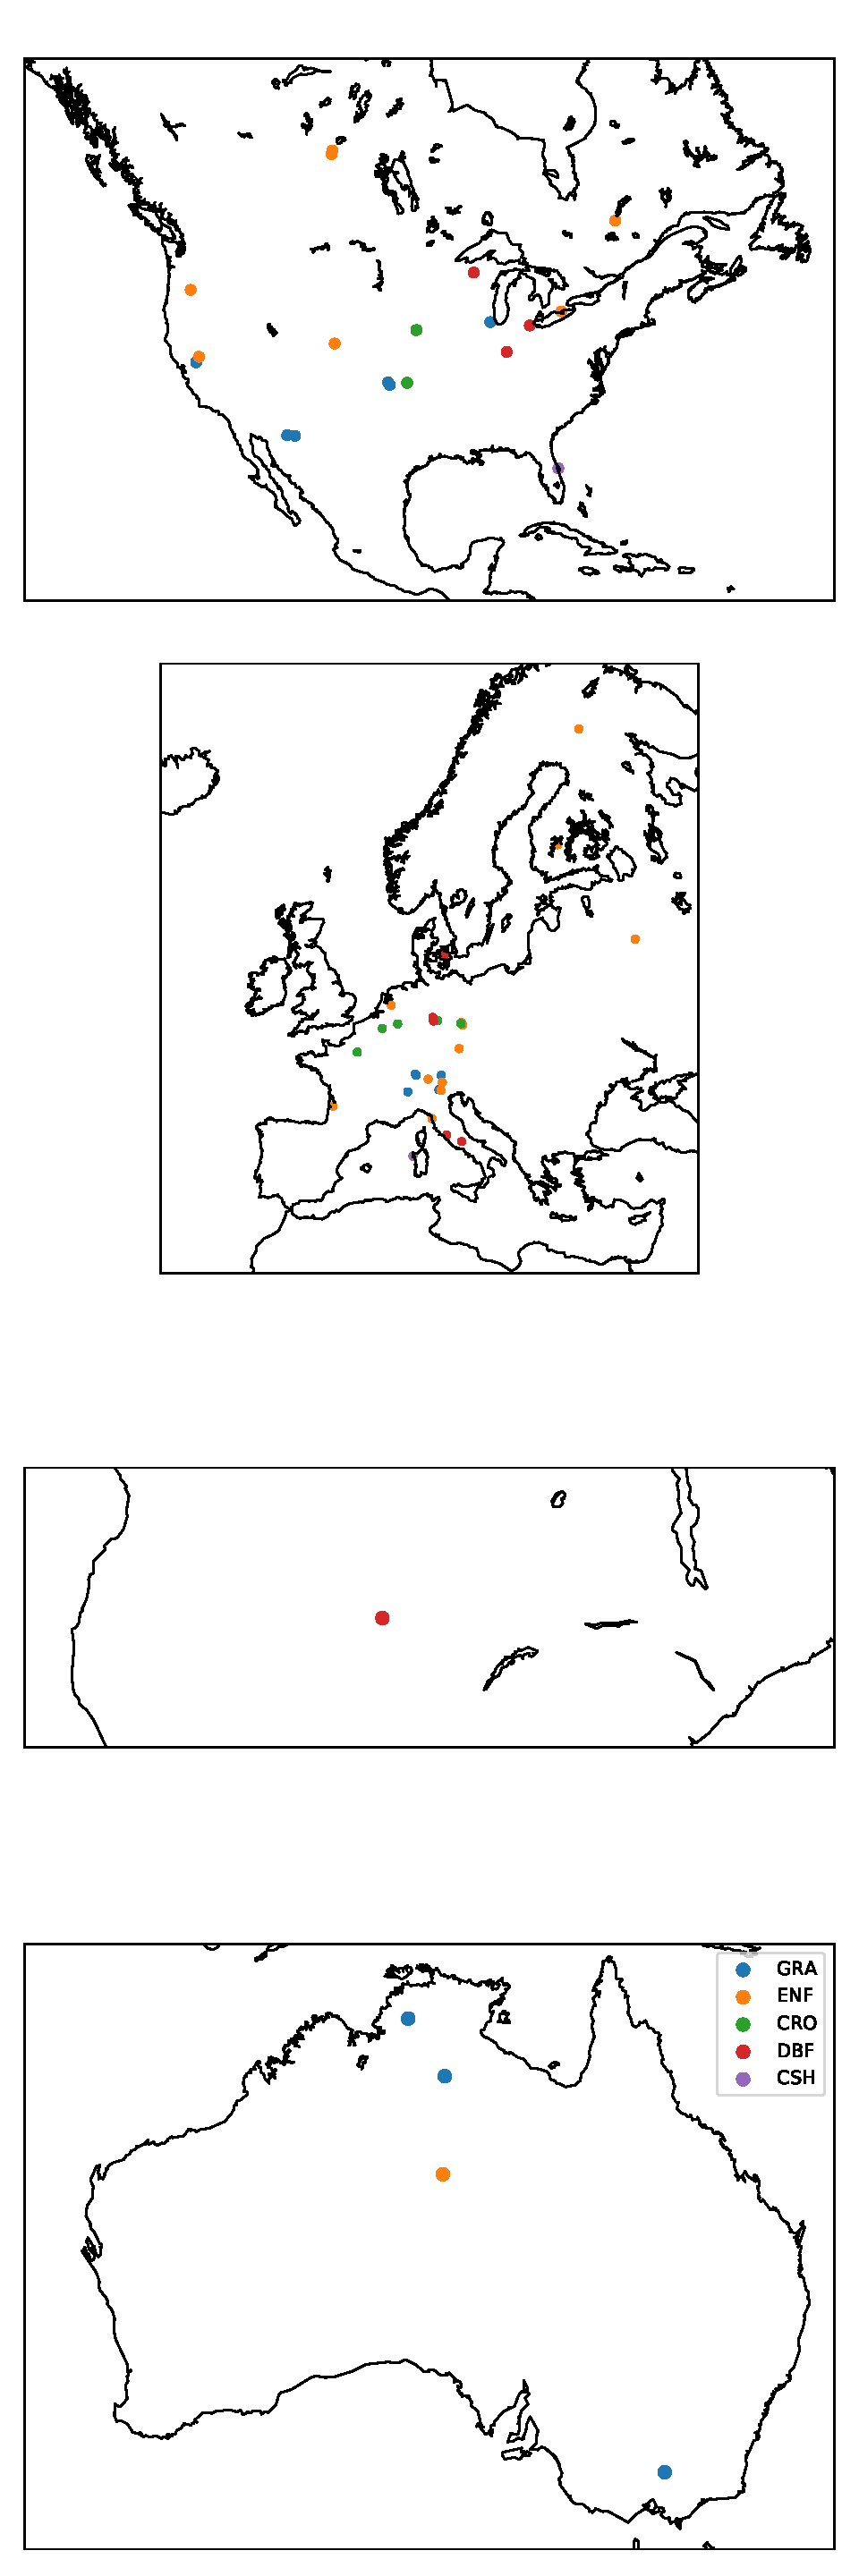
\includegraphics[width=20pc]{./fig01.pdf}
\caption{Plant functional type and location of sites used in analysis. ***\textbf{This is just  a placeholder for now, I am currently fixing it***}}
\label{map_fig}
 \end{figure}

\section{Results}
\label{results}

By construction, the variability in the $\sigma$ term (Equation \ref{sigma}) contains all model and observational uncertainties. For an observation that perfectly matches our model and constant uWUE assumption $\sigma$ will be one. Therefore, for our assumptions and framework to be reasonable $\sigma$ should be $O(1)$. Figure \ref{lai_fig} presents the histogram of calculated $\sigma$s with outliers removed (lowest and highest 5\% percent). All remaining $\sigma$ values are close to unity ($O(1)$) which provides confidence in model framework.

\begin{figure}[h]
\centering
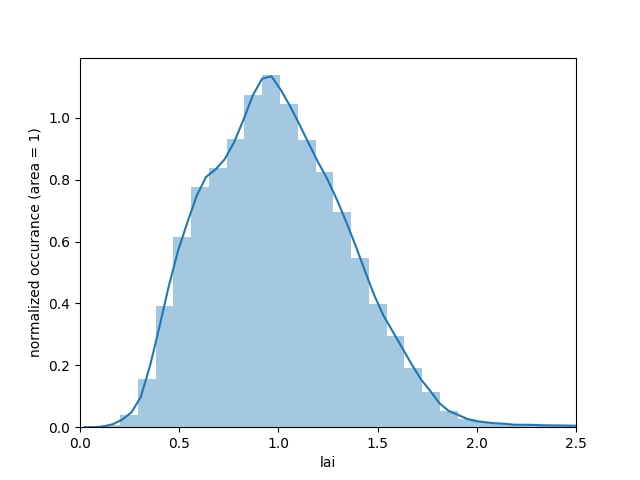
\includegraphics[width=20pc]{./fig02.png}
\caption{Histogram of $\sigma$ values calculated for each site and time according to Equation \ref{sigma}. The lowest and highest 5\% are removed as outliers, as well as any values below 0. The curve is normalized such that its area is 1. }
\label{lai_fig}
\end{figure}

An additional concern is that $\sigma$ may in fact be correlated with $VPD$, in which case the dependence would need to be accounted for when taking the derivative. Figure \ref{lai_vpd_fig} plots the joint distribution of $\sigma$ and VPD, and shows that $\sigma$ is very weakly a function of VPD. Given this weak dependence, we argue that Equation \ref{d_et} is a valid approximation for ET response to $VPD$.

\begin{figure}[h]
\centering
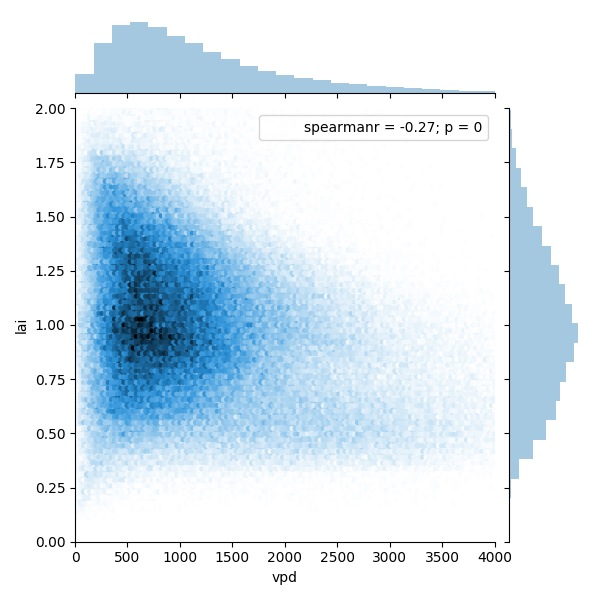
\includegraphics[width=20pc]{./fig03.png}
\caption{The joint distribution of $VPD$ and $\sigma$. $\sigma$ has only a weak dependence on $VPD$. \textbf{***note I am redoing/cleaning up this plot, ``lai'' should read sigma***}}
\label{lai_vpd_fig}
\end{figure}

Before calculating the sensitivity of ET to VPD, we will consider the functional form of Equation \ref{d_et}. There are two main terms: a ``scaling'' term, which modifies the magnitude but not the sign of the derivative $\partial ET/\partial VPD$:

\begin{equation}
  \frac{g_a \; P}{T(\Delta + \gamma)},
\end{equation}

and a ``sign'' term, which determines whether the derivative is positive i.e. atmospheric demand driven or negative i.e. physiologically controlled:

\begin{equation}
  \label{sign}
  \frac{c_p}{R_{air}} - \frac{\gamma c_s }{1.6 \; R\; \text{ uWUE }} \left( \frac{2 g_1 + \sqrt{VPD}}{2 (g_1 + \sqrt{VPD})^2}\right).
\end{equation}
All variables are positive, so the relative magnitude between the first term and the second term in Equation \ref{sign} will determine whether ET increases or decreases with increasing VPD. If the second term is larger magnitude then plant response dominates, while if the first term is larger then atmospheric demand dominates. The sign will determine whether ET is increasing or decreasing and we thus evaluate its functional form first. 

\subsection{Functional Form of the Sign Term}
\label{sign_func}
First, we explore the variables within the sign term to gain better intuition on the driver of either the increase or reduction of ET with VPD. $c_s$ and $\gamma$ are relatively constant to a good approximation so that the variability is dominated by $\sigma$ and $VPD$. $uWUE$ could vary with soil moisture but has been shown to be relatively constant except in very dry soil conditions \citep{Zhou_2016, Lin_2015}. We thus further assume that the soil is not too dry so that $uWUE$ can be approximated as a constant. This then means that the sign term only depends on VPD for a given PFT and is approximately just a function of $VPD$. We can further determine a critical threshold operating increase from decrease in ET, such that $VPD_{crit}$ where $\frac{\partial \; ET}{\partial \; VPD} = 0$:

\begin{linenomath*}
  \begin{equation}
VPD_{crit} = \frac{R_{air}}{4 c_p} \left( \frac{\gamma c_s}{1.6\; R \; \overline{\sigma} uWUE} + \sqrt{\frac{\gamma c_s}{1.6\; R \; \overline{\sigma} uWUE}\left( \frac{\gamma c_s}{1.6\; R \; \overline{\sigma} uWUE} + 8 g_1 \frac{c_p}{R_{air}}\right)} - 4 g_1 \frac{c_p}{R_{air}} \right)
\label{vpd_min_et}
  \end{equation}
\end{linenomath*}

Values of $VPD_{crit}$ as a function of PFT are shown in Table \ref{vpd_crit}. For any values of $VPD$ less than $VPD_{crit}$, $\frac{\partial \; ET}{\partial \; VPD}$ will be negative, and for values of $VPD$ greater than $VPD_{crit}$, $\frac{\partial \; ET}{\partial \; VPD}$ will be positive. In other words, ecosystems can regulate and mitigate evaporative losses up to a VPD limit, above which atmospheric demand is just too high to be entirely compensated by stomatal regulation. We note however that even though ET increases again above the critical threshold, $VPD_{crit}$, ET is still much lower that potential evaporation as stomata are stills strongly regulating vapor fluxes. Even in the absence of soil pore evaporation, stomata do not shut down entirely at very high VPD and ET does not go to zero, because stomata are still slightly open to perform some photosynthesis \citep{Ball_1987, Leuning_1990, Medlyn_2011}. In addition, upward xylem transport is necessary to maintain phloem transport and thus carbon allocation (MENCUCCINI) \explain{Not sure citation  - Comparative criteria for models of the vasuclar transport systems of tall trees}.

\begin{table}
  \label{vpd_crit}
\caption{Values of $VPD_{crit}$, where $\frac{\partial \; ET}{\partial \; VPD} = 0$, evaluated at PFT average values for $R_{air}$, $\sigma$, $\gamma$, and $c_s$. For reference, these values are also provided CITE TABLE. For values of $VPD$ less than $VPD_{crit}$, $\frac{\partial \; ET}{\partial \; VPD}$ will be negative, and for values of $VPD$ greater than $VPD_{crit}$, $\frac{\partial \; ET}{\partial \; VPD}$ will be positive. \textbf{**** this statistics are dated, need to update***}}
\centering
\begin{tabular}{l c c c c c c}
  \hline
  PFT & $R_{air}$ & $c_s$ (ppm) & $\gamma$ &  uWUE    & \textbf{$VPD_{crit}$ (Pa)} \\
  \hline
  CRO &  288.680920 & 372.567691& 65.351523& 2.602873&  \textbf{133.165438} \\
  CSH &   289.067152& 381.593622& 67.613172& 2.175278& \textbf{4439.564212} \\
  DBF &   288.624437& 377.449849& 63.421812& 2.746393&  \textbf{888.773243} \\
  ENF &  288.183849& 377.676463& 61.559242& 4.015362&  \textbf{978.084845} \\
  GRA &  288.425651& 377.264645& 61.598768& 2.281074& \textbf{1141.630778} \\
\hline
\multicolumn{2}{l}{$^{a}$Footnote text here.}
\end{tabular}
\end{table}

Differences in $uWUE$ and $g_1$ between PFTs alter the functional form of the sign term.  Larger $uWUE$ and $g_1$ will shift the sign term towards overall positive values. $g_1$ additionally plays a primary role in determining dependnece on VPD: the smaller $g_1$, the greater the $VPD$ dependence for the PFT (Figure \ref{term3}).

Based on Figure \ref{term3} and Table \ref{vpd_crit}, CROs are the least water conservative and have the most positive constant offset, while CSH are the most water conservative and have the most negative constant offset in the sign term.  ENF ($g_1 = 74.31$) has by far the largest VPD dependence of response, while CRO ($g_1 = 183.1$) has the smallest VPD dependence. This means ENF's stomatal response evolved to change substantially depending on the envionmental dryness. This contasts\explain{think about this - what does it mean - go back to Franks and think about g1's relation to wue}
 
A primary takeaway from Figure \ref{term3}a is that according to our theory for all PFTs except for crops there is frequent occurrence of a negative (plant dominating) ET response to increases in VPD. This thus means that plants are able in most atmospheric conditions to redue ET in response to increased VPD and thus to reduce water losses. To better illustrate this, the ranges of observed environmental VPDs at the FLUXNET sites are plotted parallel to the x-axis. ALL OF THIS SHOULD BE IN CAPTION NOT IN MAIN TEXT: (25th, 50th, and 75th percentiles are marked by stars), 
The location of VPD$_{crit}$ is marked by a vertical line. For CSH, VPD is always less than VPD$_{crit}$ so that the plant response dominates and empathizes the water conservative strategy of those plants. For CRO on the other, VPD is almost always higher than VPD$_{crit}$, emphasizing that those plants are water intensive and were actually engineered for photosynthesis rather than water saving. For forests and grass, whether plant response or atmospheric demand dominates is more dependent on the environment, with about half of of observed VPD less than VPD$_{crit}$, i.e. in conditions where plant response dominates. It is also important to note that even when atmospheric demand dominates, the response is still far smaller than it would be for potential evaporation i.e. atmospheric demand only, emphasizing that there is still a strong regulation of evaporative flux by stomata and though the plant xylem. The sign term in this case would just be a constant ($\frac{c_p}{R_{air}} \approx 3.5$), which is far larger than any part of the curves for any PFT. This highlights the deficiencies of PET's ability to capture land response to changes in atmospheric dryness (VPD) SEEMS TOO GENERIC BETTER EXPLAIN. However, we have assumed $\sigma$ (uncertainty) equal to one. We still need to test if inclusion of uncertainty could change our conclusions.
\begin{figure}[h]
\centering
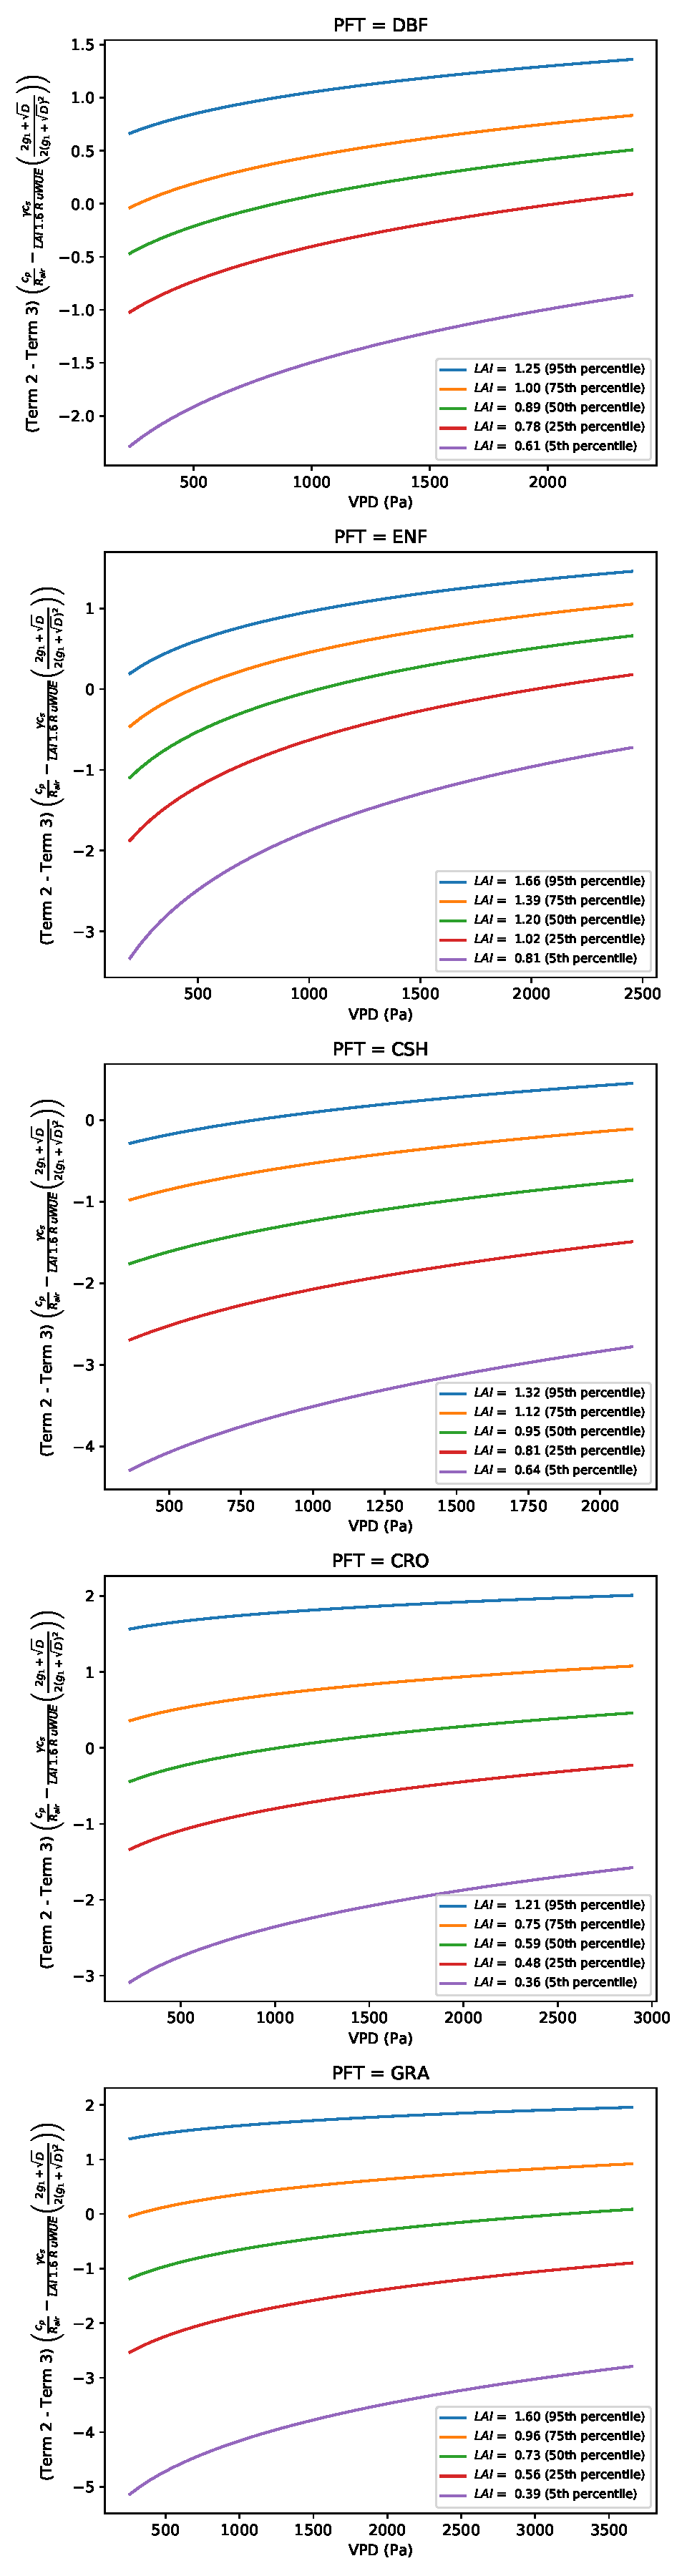
\includegraphics[width=20pc]{./fig05.pdf}
\caption{Sources of variability for the sign term. Top: sign term as a function of VPD, with $\sigma$ held fixed at 1. The observed range of VPD for each PFT is also shown below the x-axis. Line extent corresponds to 5th and 95th percentiles, while stars denote the location of the 25th, 50th, and 75th percentiles.

Bottom: The location of the minima of ET, as a function of VPD and $\sigma$. Lines and stars denote the distribution of VPD and $\sigma$ next to each axis, following the same percentiles as above. \textbf{***need to replot with correct sigma (normalized to 1), also correct uWUE label in first plot***}}
\label{term3}
\end{figure}

Figure \ref{term3}b shows the location of VPD$_{crit}$, as a function of $\sigma$ (uncertainty) and $VPD$. For any $\sigma$ or VPD less (more) than these curves, the sign term will be negative (positive). It is clear that the portion of VPD observations below/above these curves will be a strong function of $\sigma$. However, we can see some general trends. For CSH, $\frac{\partial \; ET}{\partial \; VPD}$ should be negative for the vast majority of observed $\sigma$ and VPD. The fraction of positive $\frac{\partial \; ET}{\partial \; VPD}$ appears to be more even for ENF, GRA, and DBF, and we might expect a greater frequency of positive $\frac{\partial \; ET}{\partial \; VPD}$ for CRO. Section \ref{testing} further examines the consistency of our theory, given  the apparent sensitivity to uncertainty ($\sigma$). THIS PARAGRAPH DOES NOT SEEM CONCLUSIVE AND MORE A TRAIN OF THOUGHT. LAY DOWN EXACTLY WHAT YOU HAVE IN MIND.


\subsection{Functional Form of the Scaling Term}

While the above discussion of the sign of $\frac{\partial \; ET}{\partial \; VPD}$ is important to answer our research question, the magnitude of $\frac{\partial \; ET}{\partial \; VPD}$ will also the relative magnitude of the change $\frac{\partial \; ET}{\partial \; VPD}$ and the importance of $VPD$ variability for overall $ET$ variability. So we now more closely examine the scaling term: $\frac{P}{T} \propto \rho$. Air density $\rho$ scaling term varies little relative to aerodynamic conductance and $\Delta$. The psychrometric constant $\gamma$ is also relatively constant, so the scaling term should be primarily a function of aerodynamic conductance and temperature, through the slope of the Clauisu-Clapeyron relationship $\Delta$. This is as expected, given that the aerodynamic conductance represents the efficiency fo the transfer of surface anomalies to the atmosphere. As it increases I THINK YOU REALLY MEAN CONDUCATANCE HERE - BE CAREFUL, any plant response will be communicated more strongly to the atmosphere (and vice-versa).

REMOVE ANY SNETENCES LIKE THIS MAKES SENSES ETC...

$\Delta$'s presence in the scaling term also matches physical intuition. Evaporative cooling will dampen the ability of the atmosphere to take more moisture, because $e_{s}$ decreases with decreasing temperature. The decrease in $e_{s}$ is proportional to $\Delta$ ($\delta e_{s} = \Delta \delta T$). So as $\Delta$ increases, you will get a larger damping of ET due to evaporative cooling.  The functional from of $\Delta$ will be the same across PFT, but the temperature range may vary slightly. In contrast, aerodynamic conductance will vary strongly with PFT due to the importance of surface roughness. So most of the differences in scaling between PFT should be in the aerodynamic conductance term. One interesting side note is that the coefficient of variability for both aerodynamic conductance and the scaling term is relatively constant across PFT, suggesting that the influence of aerodynamic conductance on the relative (to the PFT mean) variability of the scaling term is approximately similar across PFT.

Figure \ref{scale_vary}A shows the scaling term normalized by mean aerodynamic conductance (calculated for each plant functional type), and confirms that much of the relative variability of the scaling term is caused by aerodynamic conductance variability. Generally, temperature (via $\Delta$) causes less relative variability. However, the impact of $T$ on the relative variability increases with increasing aerodynamic conductance. 

While the relative variability of scaling term is similar across PFT, the absolute value of scaling term varies strongly across PFT. Figure \ref{scale_vary}B shows scaling term evaluated at the mean aerodynamic conductance for each PFT, and at the range of observed temperatures for each PFT. As expected, for the tree PFTs (DBF, ENF) the scaling term is much larger and the temperature dependence is much stronger. Systematic differences in observed temperatures also cause differences in the average magnitude of scaling term. For example, ENF experiences on average colder temperatures and is thus more likely to have a larger scaling term. Additionally, because the variability of aerodynamic conductance increases proportionally to the mean, the spread of the scaling term due to aerodynamic conductance variability will be larger for the tree PFTs, although this is not shown for simplicity. To summarize Figure \ref{scale_vary}: the variability of the scaling term within each PFT will look like Figure \ref{scale_vary}A for each PFT, but the scale of the y-axis will increase or decrease according to mean aerodynamic conductance observed in Figure \ref{scale_vary}B.
 
\begin{figure}[h]
\centering
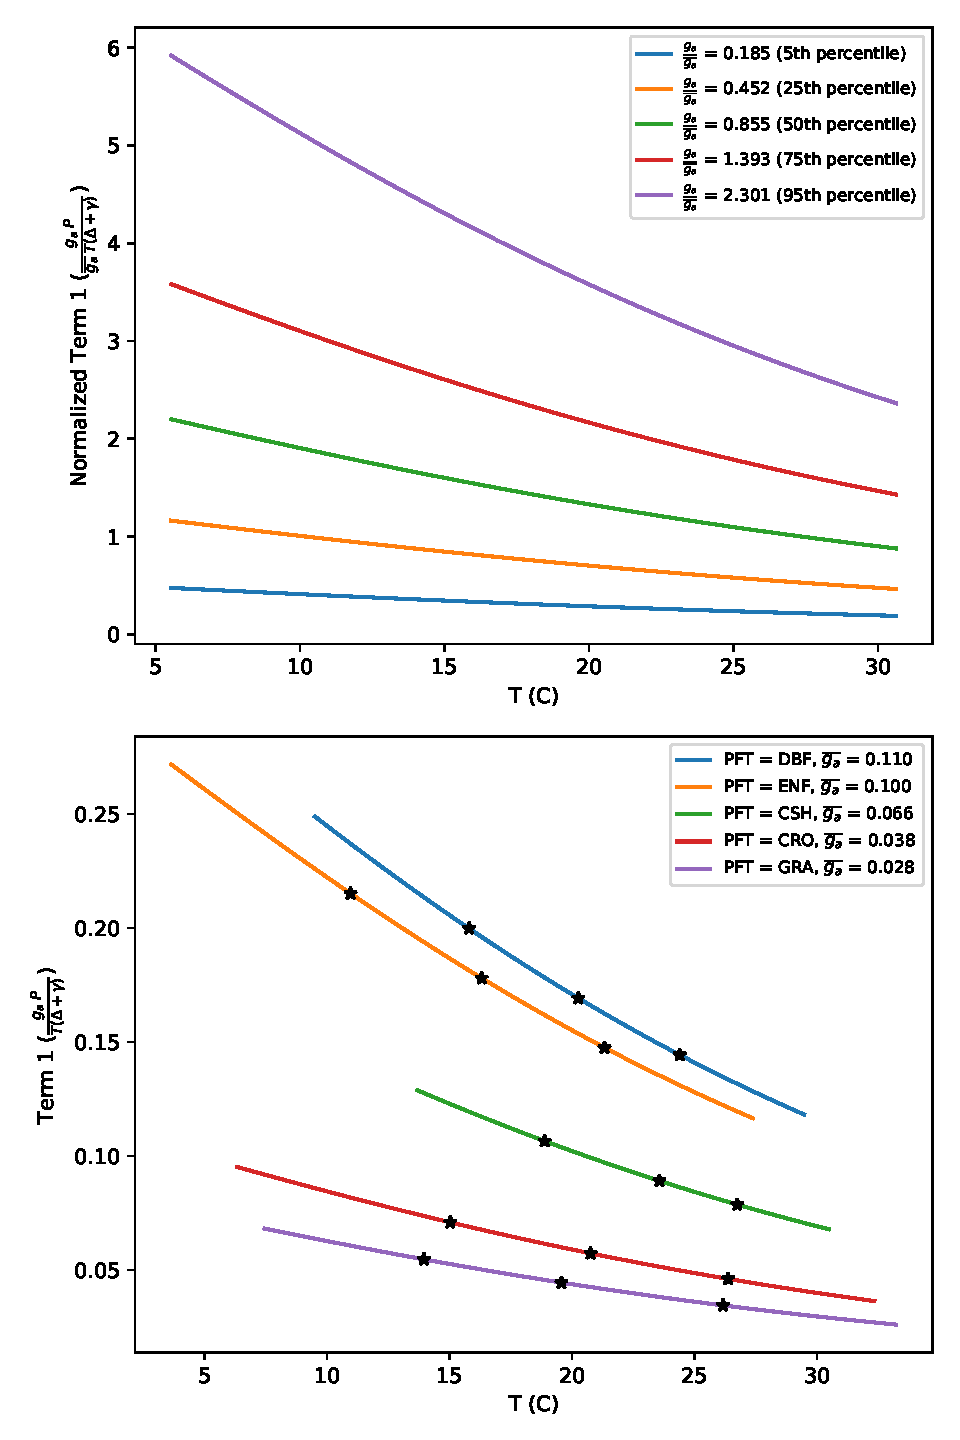
\includegraphics[width=20pc]{./fig04.pdf}
\caption{Primary sources of variability for scaling term. A) Variability within each PFT: scaling term normalized by mean $g_a$ for each PFT. B) Variability between each PFT: scaling term evaluated at mean $g_a$ for each PFT. Temperature range is 5-95th percentile for each PFT. Additionally, stars denote the location of the 25th, 50th, and 75th percentiles.}
\label{scale_vary}
\end{figure}

%%%%% replace below with idea:
\subsection{Bulk statistics of $\frac{\partial \; ET}{\partial \; VPD}$}

Table 3 confirms our expectations for PFT behavior of $\frac{\partial \; ET}{\partial \; VPD}$. For all PFTs except for CRO, average $\frac{\partial \; ET}{\partial \; VPD}$ is less than zero. However, $\frac{\partial \; ET}{\partial \; VPD}$ evaluated at the average of all variables (e.g. $\sigma$, $T$, $c_s$, $VPD$) is only negative for CSH and GRA. And, DBF in addition to CRO experiences $\frac{\partial \; ET}{\partial \; VPD}$ < 0 less than half the time. These observations highlight the effect of the nonlinear function in Figure \ref{term3}: $\frac{\partial \; ET}{\partial \; VPD}$ has a much steeper slope when the function is negative, and is thus more likely to be large magnitude.

The units of $\frac{\partial \; ET}{\partial \; VPD}$ make it difficult to interpret if $VPD$ is even a meaningful contributor to ET's variability. To better understand $VPD$'s contribution, we multiply $\frac{\partial \; ET}{\partial \; VPD}\left(\overline{env}\right)$ with $VPD$'s standard deviation to define a (linearized) relative change in ET for variations in $VPD$ . $VPD$'s contribution to ET's variability ranges between 30 - 40 W m$^{-2}$ for all PFTs except for CSH, which is about 100 W m$^{-2}$. Another meaningful comparison is to $\frac{\partial \; ET}{\partial \; R} \cdot std(R)$, as net radiation is generally the driver of ET (cite joe berry here)\explain{Find citation?}. For all PFTs except for CSH $VPD$ contributes between 30 - 40 \% of $R$'s contribution to variability. For CSH the portion is much larger, about 88 \%. $VPD$'s variability is certainly a non-negligible contributor to $ET$'s variability.

Theoretical derivation has so far illuminated the dependence of $\frac{\partial \; ET}{\partial \; VPD}$ and how it varies across PFT. Large mean $uWUE$ shifts CRO and DBF towards positive $\frac{\partial \; ET}{\partial \; VPD}$ i.e. increasing ET at higher VPD, but $\overline{\frac{\partial \; ET}{\partial \; VPD}}$ is still negative for DBF due to its lower $g_1$ SAY PHISICALLY WHAT IT IS FOR THE READER TO UNDERSTAND. ENF's low $g_1$, which is even lower than DBF, increases the dependence of $\frac{\partial \; ET}{\partial \; VPD}$ on $VPD$, and makes the function strongly nonlinear. This has the side effect of pushing $\overline{\frac{\partial \; ET}{\partial \; VPD}}$ negative further than other PFTs for a given fraction $\frac{\partial \; ET}{\partial \; VPD} < 0$ and magnitude $\frac{\partial \; ET}{\partial \; VPD}(\overline{T,\ldots,VPD})$. SAY THIS IN WORDS AS WELL OR YOU WILL LSOE THE READER. GRA shows the opposite behavior; a relatively high $g_1$  makes the function more linear, decreasing the magnitude of $\overline{\frac{\partial \; ET}{\partial \; VPD}}$ for a given fraction $\frac{\partial \; ET}{\partial \; VPD} < 0$ and negative $\frac{\partial \; ET}{\partial \; VPD}(\overline{T,\ldots,VPD})$. SAY IN WORDS AGAIN WHAT IT MEANS OTHERWISE PEOPLE WILL NOT UNDERSTAND OUR RESULTS. Finally, the low $uWUE$ of CSH pushes it toward the lowest values of $\frac{\partial \; ET}{\partial \; VPD}$ (Figure \ref{term3}) across all PFTs WHAT DOES IT MEAN AGAIN. Variability in $VPD$ accounts for the largest amount of $ET$ variability for CSH. For the other PFTs, $VPD$ contributes less to $ET$ variability, but still represents about 30-40 \% of $R$'s contributions to ET variability. WHAT IS THE SORUCE OF VARIBILITY OF THE REST OF ET I DON"T KNOW IF THAT IS RELEVANT FOR THE PRESENT PAPER.

\begin{table}
\caption{Statistics of $\frac{\partial \; ET}{\partial \; VPD}$ as a function of PFT. \textbf{***dated, need to update these statistics***}}
\centering
\begin{tabular}{l c c c c c}
  \hline
PFT & $\overline{\frac{\partial \; ET}{\partial \; VPD}}$ & $\frac{\partial \; ET}{\partial \; VPD}\left(\overline{env}\right)$ & $\frac{\partial \; ET}{\partial \; VPD}\left(\overline{env}\right)*\text{std}(VPD)$ & $\frac{\frac{\partial \; ET}{\partial \; VPD}\left(\overline{env}\right)*\text{std}(VPD)}{ \frac{\partial \; ET}{\partial \; R}\left(\overline{env}\right)*\text{std}(R)}$ & fraction $\frac{\partial \; ET}{\partial \; VPD} < 0.$ \\
  \hline
CRO & 0.000853 & 0.026241 & 37.05 & 0.41 & 0.473311\\
CSH & -0.108234 & -0.091526 & 101.72 & 0.88 & 0.931660\\
DBF & -0.012727 & 0.013794 & 39.47 & 0.33 & 0.461674\\
ENF & -0.034087 & 0.000706 & 33.22 & 0.30 & 0.534425\\
GRA & -0.019637 & -0.000921 & 33.60 & 0.35 & 0.631735\\
\hline
  
\end{tabular}
\end{table}


\subsection{Validation of theory at eddy-covariance sites}
\label{testing}
So far we have developed a theory for $\frac{\partial \; ET}{\partial \; VPD}$'s behavior as a function of VPD and PFTs. We now turn to an direct evaluation against observations taken from a wide range of eddy-covariance datasets (SEE METHODS).

Figure \ref{agu_fig} shows the distribution of of the sign term (when uncertainty is included), as compared to what the theory would predict. Our goal  was to capture the leading order behavior of the ET dependence on VPD. Given the assumptions we have made, and the uncertainties of flux tower observations themselves, we expect a large amount of noise when reprdrocuing the derivatives of ET.

ALL OF THE REST SHOULDB EB EXPLAINED IN MUCH MORE DETAIL DESCRIBE EACH FIGURE AND THE RESULTS For DBF and CSH our theory is successful towards this goal: the theory matches the leading order behavior of the function when uncertainty is included.  The plots for DBF and CSH look as one would expect if one just added noise on top of our theory.

The theory does not match as well for CRO and GRA. Perhaps this should be expected. Our theory, for practical reasons, does not include important sources of variability (particularly between sites) for CRO and GRA. We do not account for seasonal changes in LAI, variability in crop height and surface roughness, differences in C3 vs C4 photosynthesis, or differences in irrigation practices between the sites. Given that the our theory does not do as well for CRO and GRA, we will refrain from firm statements about how CRO and GRA respond to changes in VPD.

ENF is a special case. The VPD dependence of the theory is not well captured by observations. However, the theory closely captures the intercept where $\frac{\partial \; ET}{\partial \; VPD} = 0$. Resolving this feature is the key to answering our question, so perhaps the theory is still useful for ENF for the purpose of addressing when VPD drives or reduces ET. It is also noteworthy that we used published constants for $g_1$, which determines the VPD dependence, from \cite{Lin_2015}. We could have fit our own constants so that the theory would best match the observations, but our goal was to use a priori physical constants whenever possible.

While the above discussion shows that our theory has some limitations when applied to some sites, especially for crops and grasslands, another question could be, how does our theory's performance compare to often-used PET? Again, as in Section \ref{sign_func}, the PET response to changes in VPD will be constant at about 3.5. Even with uncertainty included, no values of the response approach the PET case YOU NEED TO ELABORATE WAY MORE AND GUDE THE READER THROUGH YOUR THOUGHTS. PET's status outside the error bars of our theory highlight the usefulness of our theory (and Equation \ref{et}) for estimating land response and moisture budgeting.

\subsubsection{Testing VPD$_{crit}$}
As stated in the above discussion of ENF, we are mostly interested in the critical threshold $VPD_{crit}$ for which the sign of  $\frac{\partial \; ET}{\partial \; VPD}$ is determined. When $VPD < VPD_{crit}$, $\frac{\partial \; ET}{\partial \; VPD}  < 0$ (plant response dominates), and when $VPD > VPD_{crit}$, $\frac{\partial \; ET}{\partial \; VPD} > 0$ (atmospheric demand dominates). Theoretically this $VPD_{crit}$ is only a function of PFT. We can look at how this value of $VPD_{crit}$ matches the data as different observed variables (including uncertainty) are allowed to vary.


Figure \ref{real} presents calculated $\frac{\partial \; ET}{\partial \; VPD}$ where, unless otherwise noted, all variables in Equation \ref{d_et} are allowed to vary, including uncertainty. Each column represents a different quantity related to $\frac{\partial \; ET}{\partial \; VPD}$, and each row is a different PFT. Vertical black lines denote where our theory says $VPD_{crit}$ should be. For any observations to the left of this line $\frac{\partial \; ET}{\partial \; VPD}$ should be negative (plant response dominates), and any observations the right of the line should be positive (atmospheric demand dominates). In addition to seeing how our theoretically-derived VPD threshold, $VPD_{crit}$, matches observations, these analysis DO NOT SAY PLOT OR IT SOUNDS LIKE A MSC PROJECT are also useful for observing how the scaling term affects the magnitude of the derivative, if at all. 

The scatter plots generally confirm expectations from Figure \ref{agu_fig}. By comparing different columns of Figure \ref{real} we can evaluate the impact of $\sigma$ and $g_a$ on the variability of $\frac{\partial \; ET}{\partial \; VPD}$. $g_a$'s scaling (included in columns 1 and 3) alters the magnitude considerably, particularly between PFTs. $\sigma$ variability (included in columns 1 and 2) adds a lot of additional noise to the signal of $\frac{\partial \; ET}{\partial \; VPD}$, as observed in Figure \ref{agu_fig}. However, the general story with the noise appears to match the cleaner signal when $\sigma$ is help constant and $VPD_{crit}$ is clearly visible. The exceptions are, as discussed above, for GRA and CRO, where the full complexity plots (Columns 1 and 2) do not match well with $\sigma$ held fixed (Columns 3 and 4).

While $g_a$ has a large impact on the magnitude of the scaling, temperature, through the derisive of the Clausius-Clapeyron, $\Delta$, term, does not appear to have as much of an impact in the complete estimation of $\frac{\partial \; ET}{\partial \; VPD}$. Therefore it appears that the absolute magnitude of the derivative can be mostly attributed to the sign term, and its direct scaling by aerodynamic conductance. Intuitively this is reasonable; aerodynamic conductance will control how dominant balances at the land surface are communicated to the boundary layer. While $\Delta$ controls the efficiency of latent fluxes in carrying heat away from the surface, it appears this is a second order term, relative to $g_a$, for scaling $\frac{\partial \; ET}{\partial \; VPD}$. 

In general Figures \ref{real} and \ref{agu_fig} match our expectations, even with the large sensitivity to $\sigma$ seen in Figure \ref{term3}. Our $\sigma$-based method of uncertainty propagation blurs the idealized expectations the most for GRA and CRO. We therefore have the most confidence in our conclusion based on Equation \ref{d_et} for PFTs CSH, DBF, and ENF, as the sign of the derivative with uncertainty included matches (to leading order) the story when $\sigma$ is held fixed.

\begin{figure}[h]
\centering
\includegraphics[width=\textwidth]{./agu_fig.pdf}
\caption{Comparison of the sign term with model uncertainty included (box plots) to the sign term as calculated with simplifying assumptions (blue line).}
\label{agu_fig}
\end{figure}


\begin{figure}[h]
\centering
\centerline{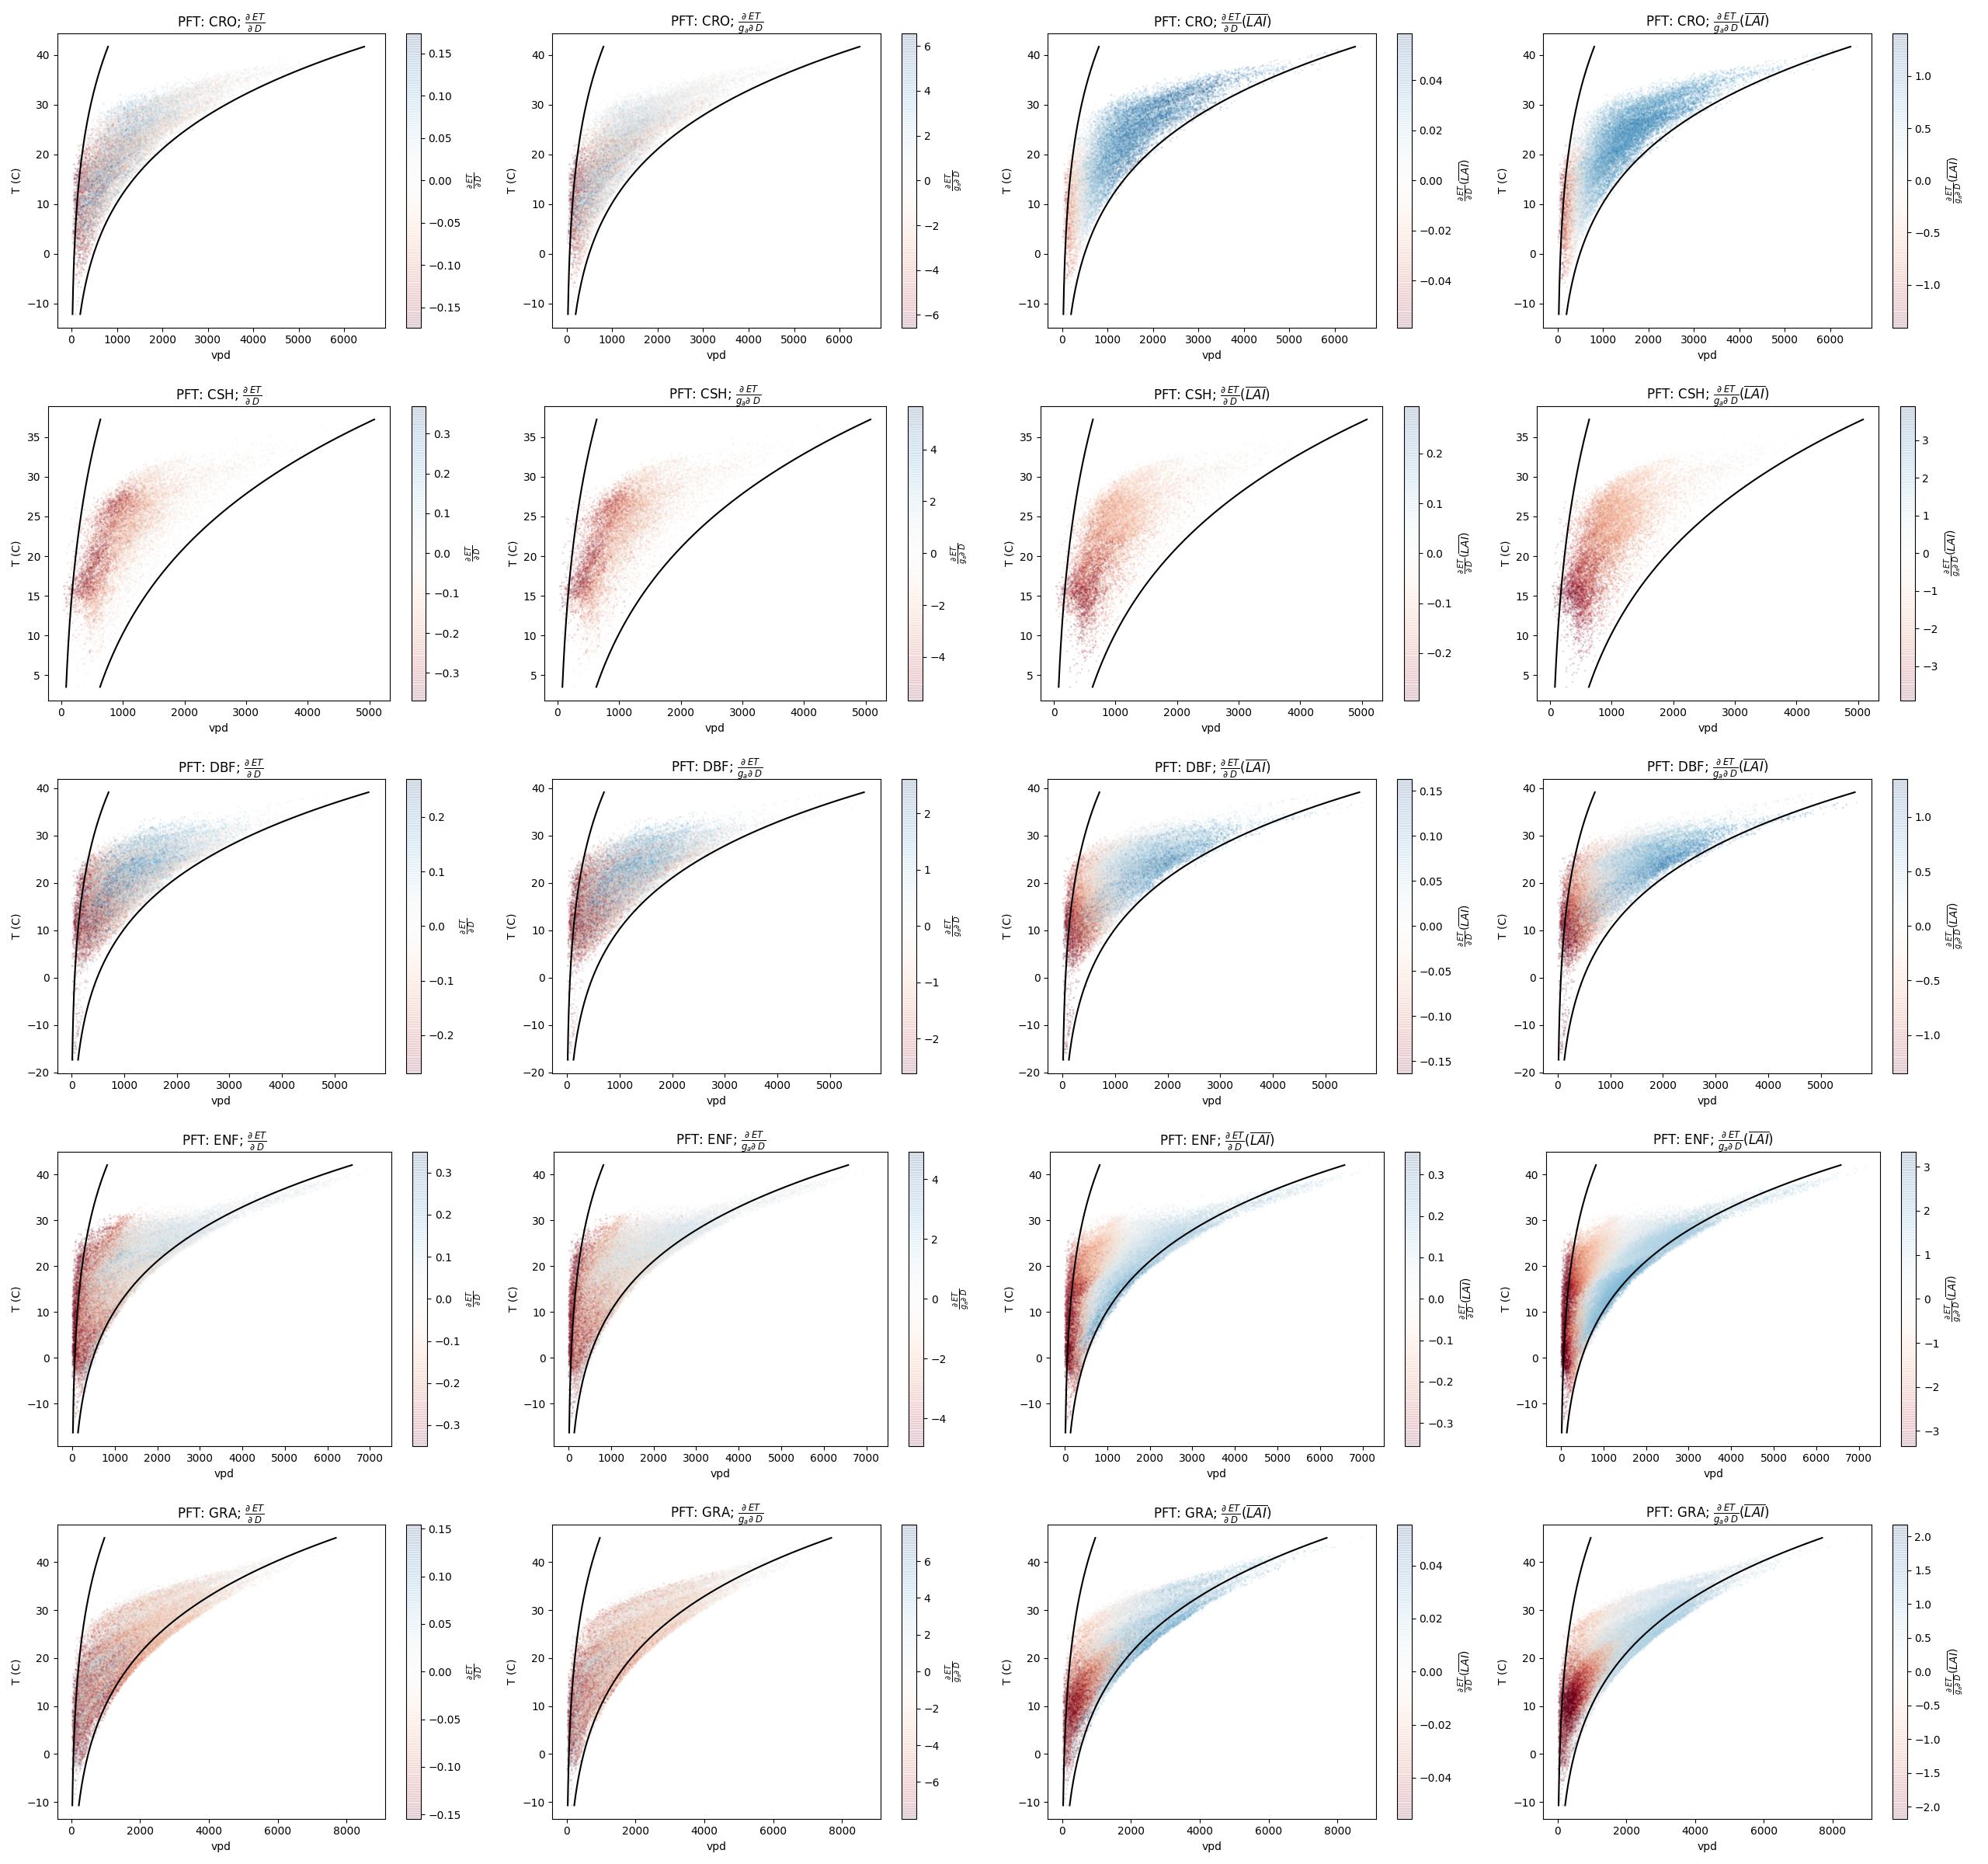
\includegraphics[width=1.4\textwidth]{./fig06.png}}
\caption{Scatter plots of $\frac{\partial \; ET}{\partial \; VPD}$. Each row is a different PFT, and each column is a different quantity related to $\frac{\partial \; ET}{\partial \; VPD}$, as labeled: Column 1: $\frac{\partial \; ET}{\partial \; VPD}$; Column 2: $\frac{\partial \; ET}{\partial \; VPD}$ normalized by $g_a$; Column 3: $\frac{\partial \; ET}{\partial \; VPD}$ with $\sigma$ held fixed at 1; and Column 4: $\frac{\partial \; ET}{\partial \; VPD}$ normalized by $g_a$ and with $\sigma$ held fixed. Please note differences in the colorbar scale.}
\label{real}
\end{figure}

% \begin{figure}[h]
% \centering
% 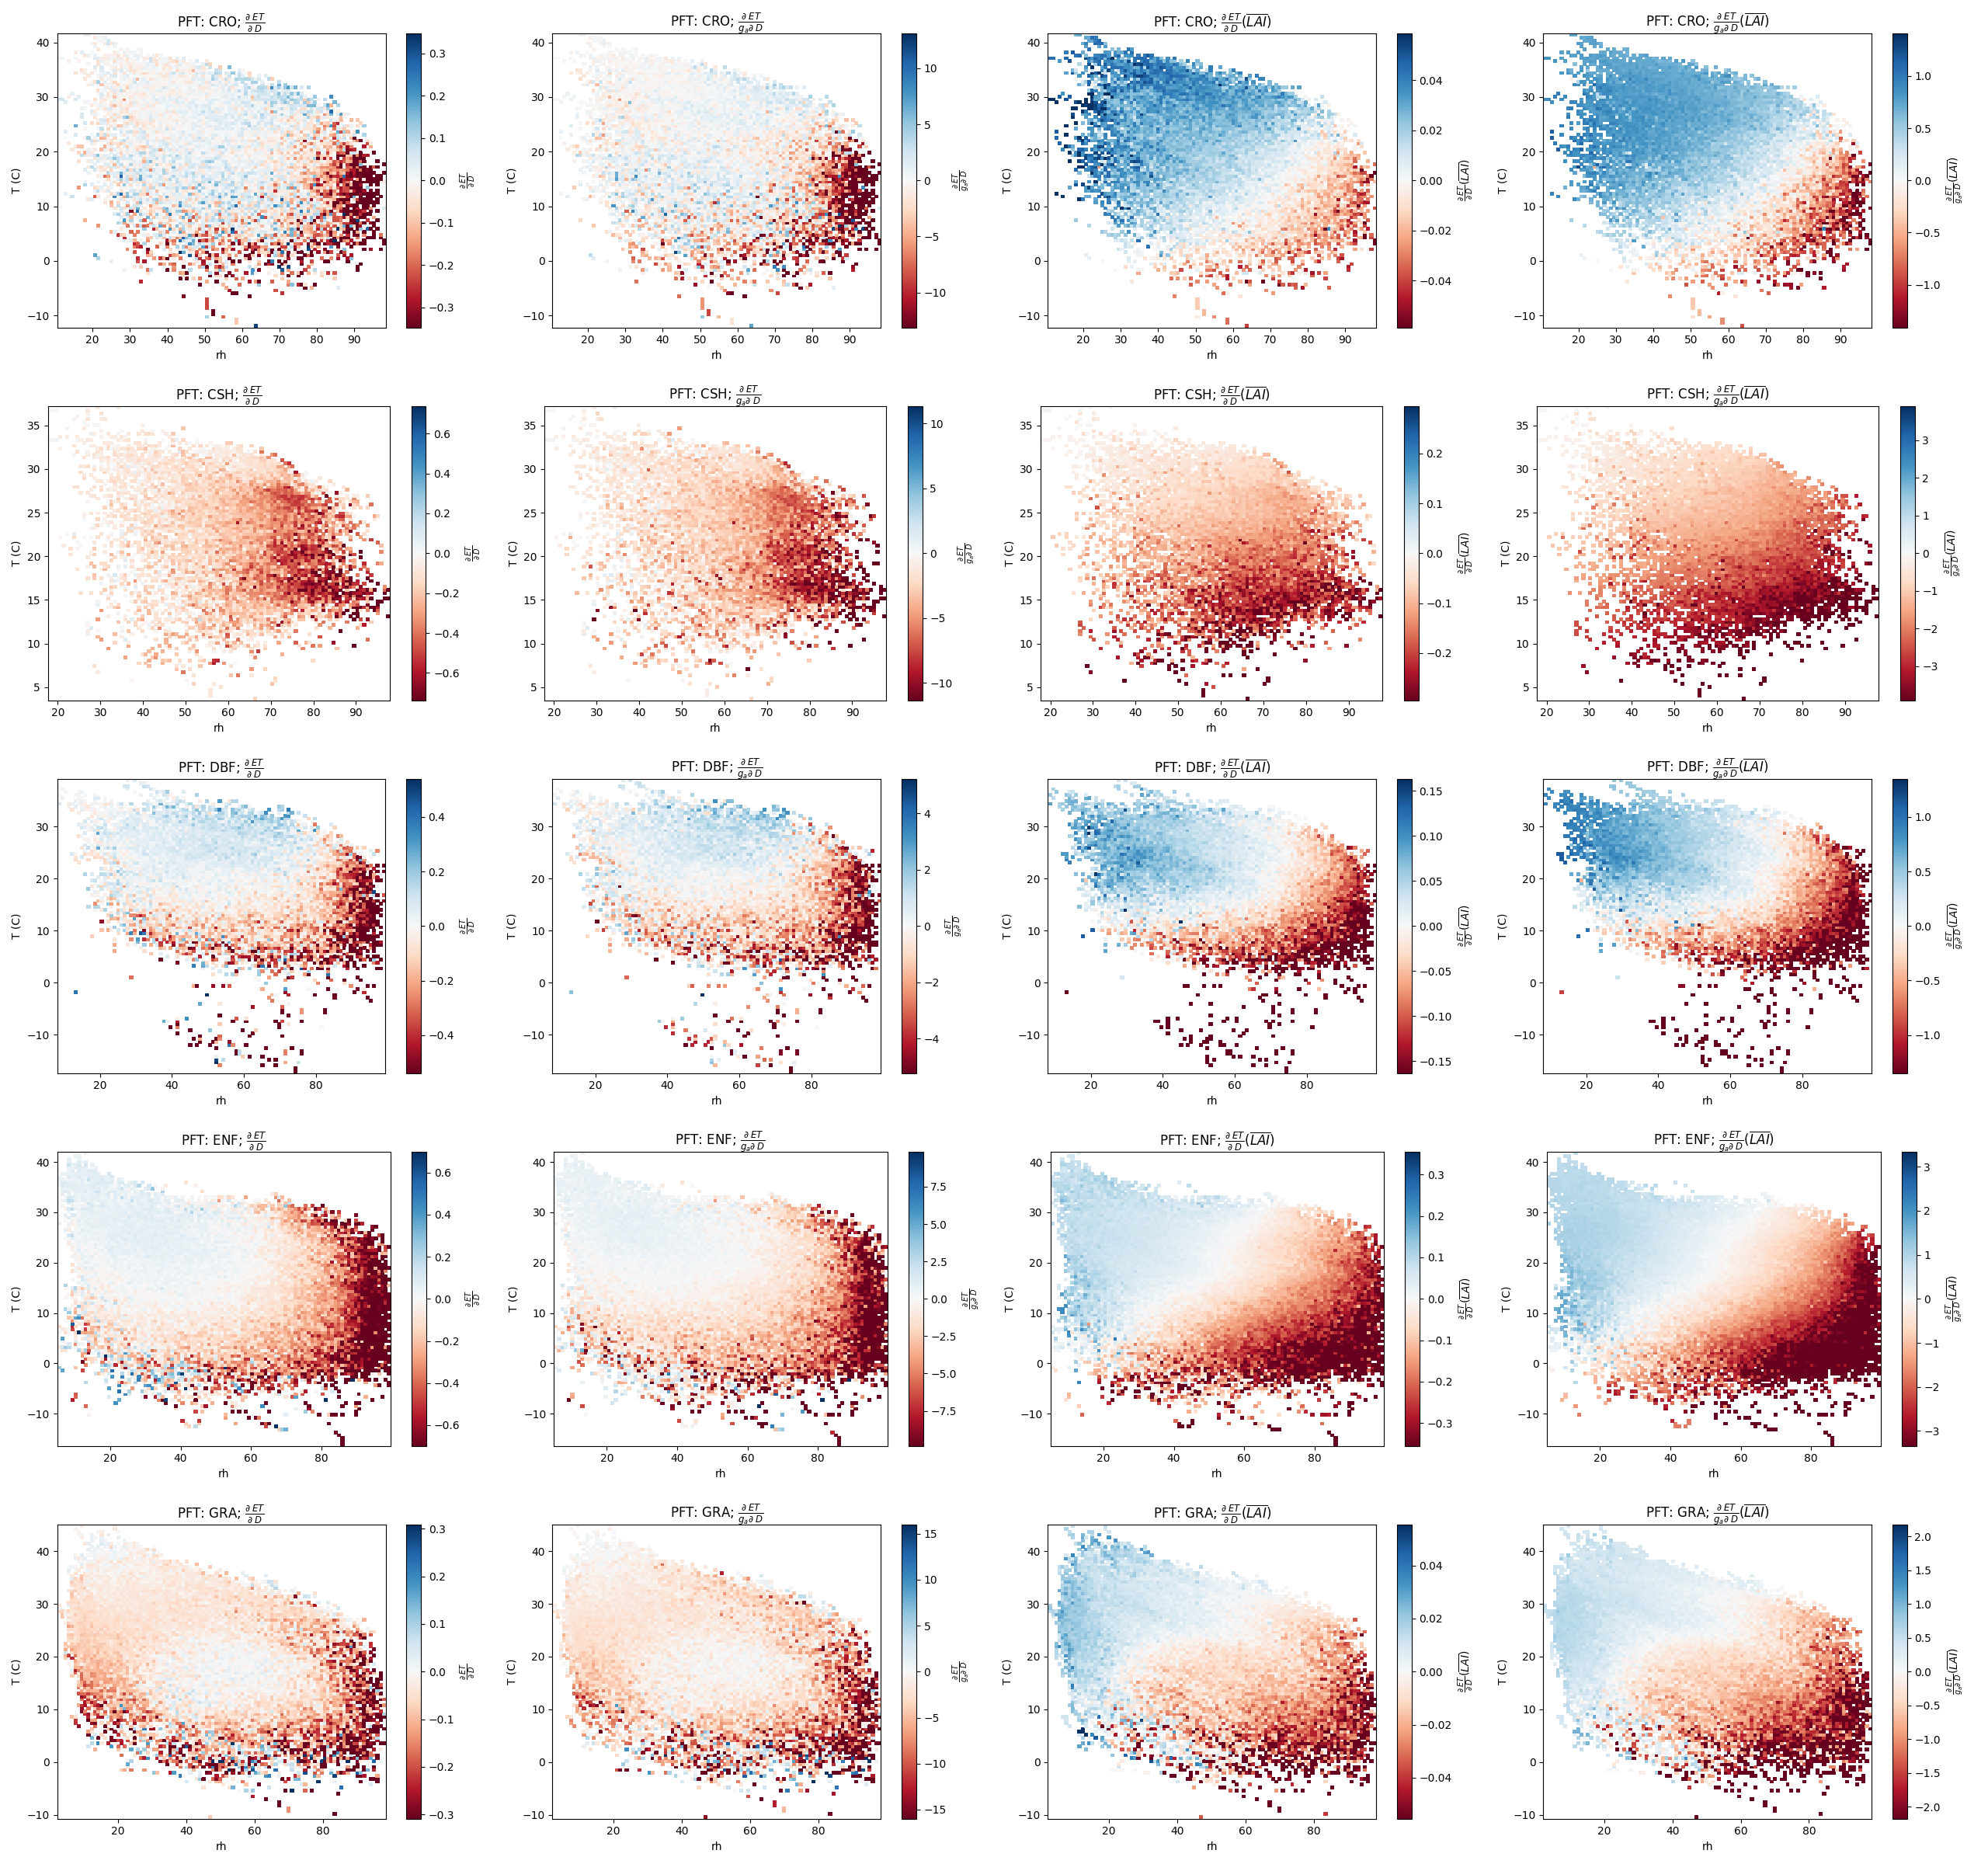
\includegraphics[width=\textwidth]{./fig06b.png}
% \caption{****alternate Fig 06****  Scatter plots of $\frac{\partial \; ET}{\partial \; VPD}$. Each row is a different PFT, and each column is a different quantity related to $\frac{\partial \; ET}{\partial \; VPD}$, as labeled. If I end up using this, I could also draw on the curve of $VPD_{crit}$ with $\overline{\frac{\text{LAI}}{\text{LAI$_{ref}$}}}$. }
% \label{real2}
% \end{figure}


HERE DISCUSS LIMITATION OF THE METHODS TO BVERY DRY CONDITIONS AND THE FEEDBCAK TO THE ATMOSPHERE OF VERY DRY SOIL CONDITIONS (BERG ET AL 2016, GENTINE ET AL> 2016)

\section{Conclusions} 

We derived a new form of Penman Monteith using $uWUE$ (\cite{Zhou_2015}) to remove the stomatal conductance term's implicit dependence on ET. With our new form of Penman Monteith we developed a theory for when an ecosystem will tend to reduce or increase ET with increasing VPD. The goal was to capture the leading order behavior of the system to gain some intrinsic knowledge for its behavior. This intuition can be used to disentangle land atmosphere feedbacks in more complicated scenarios, and will aid interpretation of observations and sophisticated models.

Our theory states that each plant type has a critical VPD below which ET will decrease (plant response dominating) and above which ET will increase (atmospheric demand dominates). We tested our theory using data from FLUXNET 2015, and found that for DBF and CSH the theory succeeds in capturing the leading order behavior. For ENF, the theory succeeds in capturing the leading order behavior for the sign of $\frac{\partial \; ET}{\partial \; VPD}$, but not for magnitude. In contrast, the model does not capture the behavior for CRO and GRA. In some ways we should have expected this, as our theory does not account for large sources of variability we would expect for those plant types, including varying surface roughness, c3 vs c4 photosynthesis, and potential differences in irrigation across sites. Given these deficiencies for CRO and GRA, we will withhold conclusions on their response to increasing VPD.

For the forest sites (DBF, ENF) the observed environmental VPD approximately straddles the critical VPD, with about half the observations below the critical VPD and half above. However for CSH the environmental VPD never exceeds the critical VPD, and even when uncertainty is included the sign of the derivative is almost always negative (93\% of observations).

While our theory predicts common occurrence of positive $\frac{\partial \; ET}{\partial \; VPD}$ (atmospheric demand dominates), the plant response is still important even when $\frac{\partial \; ET}{\partial \; VPD} > 0$. The magnitude of the ``sign term'' of our theory is always far below what it would be if we only considered the atmospheric demand term (PET). This means that any drought indices or analysis using PET will not capture how the vegetated surface respond and react to increases in atmospheric demand. However, the new uWUE-version of Penman Monteith we derived (Equation \ref{et}) could be used as a complement to PET in drought indices. One could calculate and compare indices  when plant response is ignored (PET) or included (Equation \ref{et}). 

This paper provides initial intuition for how the land surface responds to atmospheric drying. This intuition for the one-way behavior of  land surface response to atmospheric drying is critical first step to disentangling land-atmosphere feedbacks at various scales, from diurnal to seasonal and beyond. 

%%
%% Enter Figures and Tables near as possible to where they are first mentioned:
%
% DO NOT USE \psfrag or \subfigure commands.
%
% Figure captions go below the figure.
% Table titles go above tables;  other caption information
%  should be placed in last line of the table, using
% \multicolumn2l{$^a$ This is a table note.}
%
%----------------
% EXAMPLE FIGURE
%
% \begin{figure}[h]
% \centering
% when using pdflatex, use pdf file:
% \includegraphics[width=20pc]{figsamp.pdf}
%
% when using dvips, use .eps file:
% \includegraphics[width=20pc]{figsamp.eps}
%
% \caption{Short caption}
% \label{figone}
%  \end{figure}
%
% ---------------
% EXAMPLE TABLE
%
% \begin{table}
% \caption{Time of the Transition Between Phase 1 and Phase 2$^{a}$}
% \centering
% \begin{tabular}{l c}
% \hline
%  Run  & Time (min)  \\
% \hline
%   $l1$  & 260   \\
%   $l2$  & 300   \\
%   $l3$  & 340   \\
%   $h1$  & 270   \\
%   $h2$  & 250   \\
%   $h3$  & 380   \\
%   $r1$  & 370   \\
%   $r2$  & 390   \\
% \hline
% \multicolumn{2}{l}{$^{a}$Footnote text here.}
% \end{tabular}
% \end{table}

%% SIDEWAYS FIGURE and TABLE 
% AGU prefers the use of {sidewaystable} over {landscapetable} as it causes fewer problems.
%
% \begin{sidewaysfigure}
% \includegraphics[width=20pc]{figsamp}
% \caption{caption here}
% \label{newfig}
% \end{sidewaysfigure}
% 
%  \begin{sidewaystable}
%  \caption{Caption here}
% \label{tab:signif_gap_clos}
%  \begin{tabular}{ccc}
% one&two&three\\
% four&five&six
%  \end{tabular}
%  \end{sidewaystable}

%% If using numbered lines, please surround equations with \begin{linenomath*}...\end{linenomath*}
%\begin{linenomath*}
%\begin{equation}
%y|{f} \sim g(m, \sigma),
%\end{equation}
%\end{linenomath*}

%%% End of body of article

%%%%%%%%%%%%%%%%%%%%%%%%%%%%%%%%
%% Optional Appendix goes here
%
% The \appendix command resets counters and redefines section heads
%
% After typing \appendix
%
%\section{Here Is Appendix Title}
% will show
% A: Here Is Appendix Title
%
%\appendix
%\section{Here is a sample appendix}

%%%%%%%%%%%%%%%%%%%%%%%%%%%%%%%%%%%%%%%%%%%%%%%%%%%%%%%%%%%%%%%%
%
% Optional Glossary, Notation or Acronym section goes here:
%
%%%%%%%%%%%%%%  
% Glossary is only allowed in Reviews of Geophysics
%  \begin{glossary}
%  \term{Term}
%   Term Definition here
%  \term{Term}
%   Term Definition here
%  \term{Term}
%   Term Definition here
%  \end{glossary}

%
%%%%%%%%%%%%%%
% Acronyms
%   \begin{acronyms}
%   \acro{Acronym}
%   Definition here
%   \acro{EMOS}
%   Ensemble model output statistics 
%   \acro{ECMWF}
%   Centre for Medium-Range Weather Forecasts
%   \end{acronyms}

%
%%%%%%%%%%%%%%
% Notation 
%   \begin{notation}
%   \notation{$a+b$} Notation Definition here
%   \notation{$e=mc^2$} 
%   Equation in German-born physicist Albert Einstein's theory of special
%  relativity that showed that the increased relativistic mass ($m$) of a
%  body comes from the energy of motion of the body—that is, its kinetic
%  energy ($E$)—divided by the speed of light squared ($c^2$).
%   \end{notation}




%%%%%%%%%%%%%%%%%%%%%%%%%%%%%%%%%%%%%%%%%%%%%%%%%%%%%%%%%%%%%%%%
%
%  ACKNOWLEDGMENTS
%
% The acknowledgments must list:
%
% •	All funding sources related to this work from all authors
%
% •	Any real or perceived financial conflicts of interests for any
%	author
%
% •	Other affiliations for any author that may be perceived as
% 	having a conflict of interest with respect to the results of this
% 	paper.
%
% •	A statement that indicates to the reader where the data
% 	supporting the conclusions can be obtained (for example, in the
% 	references, tables, supporting information, and other databases).
%
% It is also the appropriate place to thank colleagues and other contributors. 
% AGU does not normally allow dedications.


\acknowledgments
This work used eddy covariance data acquired and shared by the FLUXNET community, including these networks: AmeriFlux, AfriFlux, AsiaFlux, CarboAfrica, CarboEuropeIP, CarboItaly, CarboMont, ChinaFlux, Fluxnet-Canada, GreenGrass, ICOS, KoFlux, LBA, NECC, OzFlux-TERN, TCOS-Siberia, and USCCC. The ERA-Interim reanalysis data are provided by ECMWF and processed by LSCE. The FLUXNET eddy covariance data processing and harmonization was carried out by the European Fluxes Database Cluster, AmeriFlux Management Project, and Fluxdata project of FLUXNET, with the support of CDIAC and ICOS Ecosystem Thematic Center, and the OzFlux, ChinaFlux and AsiaFlux offices.


%% ------------------------------------------------------------------------ %%
%% Citations

% Please use ONLY \citet and \citep for reference citations.
% DO NOT use other cite commands (e.g., \cite, \citeyear, \nocite, \citealp, etc.).


%% Example \citet and \citep:
%  ...as shown by \citet{Boug10}, \citet{Buiz07}, \citet{Fra10},
%  \citet{Ghel00}, and \citet{Leit74}. 

%  ...as shown by \citep{Boug10}, \citep{Buiz07}, \citep{Fra10},
%  \citep{Ghel00, Leit74}. 

%  ...has been shown \citep [e.g.,][]{Boug10,Buiz07,Fra10}.



%%  REFERENCE LIST AND TEXT CITATIONS
%
% Either type in your references using
%
% \begin{thebibliography}{}
% \bibitem[{\textit{Kobayashi et~al.}}(2003)]{R2013} Kobayashi, T.,
% Tran, A.~H., Nishijo, H., Ono, T., and Matsumoto, G.  (2003).
% Contribution of hippocampal place cell activity to learning and
% formation of goal-directed navigation in rats. \textit{Neuroscience}
% 117, 1025--1035.
%
% \bibitem{}
% Text
% \end{thebibliography}
%
%%%%%%%%%%%%%%%%%%%%%%%%%%%%%%%%%%%%%%%%%%%%%%%
% Or, to use BibTeX:
%
% Follow these steps
%
% 1. Type in \bibliography{<name of your .bib file>} 
%    Run LaTeX on your LaTeX file.
%
% 2. Run BiBTeX on your LaTeX file.
%
% 3. Open the new .bbl file containing the reference list and
%   copy all the contents into your LaTeX file here.
%
% 4. Run LaTeX on your new file which will produce the citations.
%
% AGU does not want a .bib or a .bbl file. Please copy in the contents of your .bbl file here.
%\bibliography{references.bib}
% 11/23/2015
\documentclass[draft,linenumbers]{agujournal}
% \draftfalse
\usepackage{makecell}
\drafttrue

\journalname{Agricultural and Forest Meteorology}

\begin{document}

%% ------------------------------------------------------------------------ %%
%  Title
% 
% (A title should be specific, informative, and brief. Use
% abbreviations only if they are defined in the abstract. Titles that
% start with general keywords then specific terms are optimized in
% searches)
%
%% ------------------------------------------------------------------------ %%

% Example: \title{This is a test title}

\title{When does vapor pressure deficit drive or reduce evapotranspiration?}

%% ------------------------------------------------------------------------ %%
%
%  AUTHORS AND AFFILIATIONS
%
%% ------------------------------------------------------------------------ %%

% Authors are individuals who have significantly contributed to the
% research and preparation of the article. Group authors are allowed, if
% each author in the group is separately identified in an appendix.)

% List authors by first name or initial followed by last name and
% separated by commas. Use \affil{} to number affiliations, and
% \thanks{} for author notes.  
% Additional author notes should be indicated with \thanks{} (for
% example, for current addresses). 

% Example: \authors{A. B. Author\affil{1}\thanks{Current address, Antartica}, B. C. Author\affil{2,3}, and D. E.
% Author\affil{3,4}\thanks{Also funded by Monsanto.}}

\authors{A. Massmann\affil{1}, P. Gentine\affil{1}, C. Lin\affil{1,2}}


% \affiliation{1}{First Affiliation}
% \affiliation{2}{Second Affiliation}
% \affiliation{3}{Third Affiliation}
% \affiliation{4}{Fourth Affiliation}

\affiliation{1}{Department of Earth and Environmental Engineering, Columbia University, New York, NY 10027}
\affiliation{2}{Department of Hydraulic Engineering, Tsinghua University, Beijing, CN}

  % (repeat as many times as is necessary)

%% Corresponding Author:
% Corresponding author mailing address and e-mail address:

% (include name and email addresses of the corresponding author.  More
% than one corresponding author is allowed in this LaTeX file and for
% publication; but only one corresponding author is allowed in our
% editorial system.)  

% Example: \correspondingauthor{First and Last Name}{email@address.edu}

\correspondingauthor{Adam Massmann}{akm2203@columbia.edu}

%% Keypoints, final entry on title page.

% Example: 
% \begin{keypoints}
% \item	List up to three key points (at least one is required)
% \item	Key Points summarize the main points and conclusions of the article
% \item	Each must be 100 characters or less with no special characters or punctuation 
% \end{keypoints}

%  List up to three key points (at least one is required)
%  Key Points summarize the main points and conclusions of the article
%  Each must be 100 characters or less with no special characters or punctuation 

\begin{keypoints}
\item = enter point 1 here = 
\item = enter point 2 here = 
\item = enter point 3 here = 
\end{keypoints}

%% ------------------------------------------------------------------------ %%
%
%  ABSTRACT
%
% A good abstract will begin with a short description of the problem
% being addressed, briefly describe the new data or analyses, then
% briefly states the main conclusion(s) and how they are supported and
% uncertainties. 
%% ------------------------------------------------------------------------ %%

%% \begin{abstract} starts the second page 

\begin{abstract}
= enter abstract here =
\end{abstract}


%% ------------------------------------------------------------------------ %%
%
%  TEXT
%
%% ------------------------------------------------------------------------ %%

%%% Suggested section heads:
% \section{Introduction}
% 
% The main text should start with an introduction. Except for short
% manuscripts (such as comments and replies), the text should be divided
% into sections, each with its own heading. 

% Headings should be sentence fragments and do not begin with a
% lowercase letter or number. Examples of good headings are:

% \section{Materials and Methods}
% Here is text on Materials and Methods.
%
% \subsection{A descriptive heading about methods}
% More about Methods.
% 
% \section{Data} (Or section title might be a descriptive heading about data)
% 
% \section{Results} (Or section title might be a descriptive heading about the
% results)
% 
% \section{Conclusions}


\section{Introduction}


Vapor pressure deficit (VPD) is expected to rise over continents in the future due to the combination of increased temperature and relative humidity drying\explain{Is increased RH conclusive and universal?- I'm not so sure... is there another citation? I don't think Byrne 2013 shows that.} \citep{Byrne_2013}.. In turn VPD modifies the atmospheric demand of evapotranspiration (ET) (Penman Monteith) but is also a stressor for stomata \citep{Leuning_1990, MEDLYN_2011}.

Answering the question ``When does vapor pressure deficit drive or reduce evapotranspiration?'' is thus motivated by two potential but opposing perspectives on the matter. The first, hydrometeorological, perspective is that higher vapor pressure deficit increases atmospheric demand for water from the land surface, and this drives an increase in evapotranspiration (ET). This perspective is particularly relevant because potential evapotranspiration (PET), which is used in many drought indices and hydrometeorological studies, only quantifies atmospheric demand effects. On the other hand, there is another perspective for vegetated surfaces. Plants' stomata have evolved to optimally regulate the exchange of water and carbon, and tend to close in response to increased atmospheric dryness \citep{Ball_1987, Leuning_1990, MEDLYN_2011}.  Therefore, an increase in VPD, in well watered soil conditions, may actually correspond to a decrease in ET because of stomatal closure. This decrease in ET would reduce and potentially cancel (in case of full closure) the effects of shifts to atmospheric demand. In other words, the  question ``When does VPD drive or reduce ET?'' can be related to whether plant regulation or atmospheric demand dominate ET. If plant response reduces ET in response to atmospheric drying then soil moisture will be better conserved. This would seem a sensible evolutionary strategy to cope with aridity. If stomata were fully passive \citep [similar to soil pores, e.g. ][]{Or_2013}, increased atmospheric aridity would further reduce soil moisture. In turn, this would further increase aridity as low soil moisture levels increase the Bowen ratio, and in turn increase temperature and reduce atmospheric humidity (gentine et al. GRL 2016, Berg 2016).  This however would not seem to be a sensible strategy for plants from an evolutionary standpoint.

First, whether VPD drives or reduces ET should be a function of plant type. Plants that evolved to conserve water (e.g. arid shrubs) will be more likely to reduce ET with increasing VPD, and plants that have evolved to care little about water (e.g. crops) will be more likely to increase ET with increasing VPD. Atmospheric conditions must matter as well. At the ecosystem scale there are limits to the strategies plants use to hold water back from the atmosphere. As atmospheric demand for water (VPD) increases, ecosystems will begin to reach their water conservation limits. At this stage any further increase in VPD will most likely drive an increase in ET, because there is little more the plants can do keep water back. 

The objective of the present manuscript is thus to evaluate the VPD dependence of ET, in non-extreme soil drought conditions. The goal of this paper is to use reasonable approximations as a tool to increase intuition for plant response to atmospheric drying. This intuition will aid interpretation of observations and full complexity models. In order to quantify plant response to perturbations in VPD, we apply a Penman-Monteith framework to derive theoretical response of ET to VPD. The model is then validated and tested at multiple eddy-covariance stations spanning various climates and plant functional types. Section 2 describes the data used. Section 3 derives the framework. Section 4 presents results and comparison to observations. Section 5 discusses conclusions. 

\section{Data}
\label{data}
We use both meterological and turbulent flux data from the FLUXNET2015 database, including all sites with more than four years of data\explain{Pierre says ``be as precise as possible,'' but not sure what he means}. Each site's plant functional type (PFT) was classified using the International Geosphere-Biosphere Programme vegetation classification scheme \citep{Loveland_1999}. The physical constants used in Section \ref{methods} are only published for five plant functional types (PFTs) crops (CRO), deciduous broadleaf forest (DBF), evergreen needleleaf forest (ENF), grass (GRA), and closed shrub (CSH) (see Table \ref{pft}). There are 56 sites with these plant functional types, and their location is shown in  Figure \ref{map_fig} \explain{map needs to be improved - it's a placeholder for now}.

The purpose of this study is to examine ecosystem response to atmospheric drying during the growing season. To accomplish this, we filter and quality control the data using a similar procedure as \cite{Zhou_2015}:
\begin{itemize}
\item Only measured or highest (``good'') quality gapfilled data, according to quality control flags, are used.
\item To isolate the growing season, we only use days in which the average GPP exceeds 10\% of the observed 95th percentile of GPP for a given site. GPP is calculated using the nighttime respiration partitioning method.
\item We remove days with rain and the day following to avoid issues with rain interception and sensor saturation at high relative humidity (\cite{MEDLYN_2011}).
\end{itemize}
Additionally, we restrict data to the daytime, which is identified when downwelling shortwave radiation is greater than 50 W m$^{-2}$ and sensible heat flux is greater than 5 W m$^{-2}$. To further reduce the chance of sensor saturation at high relative humidity, we remove all time steps for which VPD is less than .01 kPa. Timesteps with negative observed GPP or ET are also removed, and we aggregate half hourly data to hourly averages to reduce noise. After these quality control procedures, 332556 upscaled hourly observations remain. 

\section{Methods}
\label{methods}
The Penman-Monteith equation (hereafter PM \explain{find pm ciatation in shuttlewroth}) estimates ET as a function of observable atmospheric variables and surface conductances:
\begin{linenomath*}
  \begin{equation}
      ET = \frac{\Delta R + g_a \rho_a c_p VPD}{\Delta + \gamma(1 + \frac{g_a}{g_s})},
  \end{equation}
\end{linenomath*}
where variable definitions are given in Table 1. \citet{MEDLYN_2011} developed a model for stomatal conductance ($g_s$) by combining optimal photosynthesis theory \citep{Farquhar_1980, Katul_2010} with empirical approaches, which describes the dependence of $g_s$ to VPD. The result for leaf-scale stomatal conductance was:

\begin{linenomath*}
  \begin{equation}
  g_{l-s} = g_0 + 1.6 \left(1 + \frac{g_1}{\sqrt{VPD}}\right) \frac{A}{c_s}
  \end{equation}
\end{linenomath*}
This model has been shown to behave very well across PFTs, compared to other models \citep{Lin_2015}.

This can be adapted to the ecosystem scale by multiplying by leaf area index (LAI) and converting units to m s$^{-1}$:

\begin{linenomath*}
  \label{medlyn}
  \begin{equation}
  g_s = \text{LAI} \frac{R \,T}{P} \left( g_0 + 1.6 \left(1 + \frac{g_1}{\sqrt{VPD}}\right) \frac{A}{c_s}\right)
  \end{equation}
\end{linenomath*}

While Equation 3 can be used in PM (equation 1), it will make analytical work with the function intractable because $A$, net CO$_2$ assimilation, is functionally related to ET itself. To remove the dependence of ET on $A$ we can use the semi-empirical results of \citet{Zhou_2015}. \citet{Zhou_2015} showed that the underlying Water Use Efficiency $uWUE$:

\begin{linenomath*}
  \begin{equation}
    \label{uwue}
uWUE = \frac{GPP \cdot \sqrt{VPD}}{ET}
  \end{equation}
\end{linenomath*}
is relatively constant across time and space (within plant functional type). If, following \citet{Lin_2015}, we approximate $g_0$ as $0$ (i.e. we neglect cuticular and epidermal losses - a reasonable assumption except in very dry conditions), we can use uWUE to remove $A$ from $g_s$ in a way that makes PM analytically tractable:

\begin{linenomath*}
  \begin{equation}
  g_s = \frac{R \, T}{P} 1.6 \left(1 + \frac{g_1}{\sqrt{VPD}}\right) \frac{uWUE \; ET}{c_s \; \sqrt{VPD}}
  \end{equation}
\end{linenomath*}

Note that $uWUE$ is fit on the ecosystem scale in \citet{Zhou_2015} so GPP in \ref{uwue} is really $A\cdot \text{LAI}$. This leads to the cancelation of LAI in addition to uWUE in Equation \ref{medlyn}. Plugging Equation 5 into Equation 1 and rearranging gives a new expression for ET directly as a function of VPD:

\begin{linenomath*}
  \begin{equation}
    ET = \frac{\Delta R + \frac{g_a\; P}{T} \left( \frac{ c_p VPD}{R_{air}} -  \frac{\gamma c_s \sqrt{VPD} }{ R* \; 1.6\; \text{ uWUE } (1 + \frac{g_1}{\sqrt{VPD}})} \right) }{ \Delta + \gamma}
    \label{et}
  \end{equation}
\end{linenomath*}

Given FLUXNET data described in Section \ref{data}, every term in Equation \ref{et} is known. However, our sampling of sites at the global scale may introduce some deviations of $uWUE$ from those observed in \citet{Zhou_2015}. Also, we wish to include some measure of uncertainty in our analysis to check whether our assumptions and simplifications are reasonable. To account for both mean deviations of $uWUE$ and uncertainty, we will introduce an uncertainty parameter $\sigma$ modifying $uWUE$:

\begin{linenomath*}
  \begin{equation}
    ET = \frac{\Delta R + \frac{g_a\; P}{T} \left( \frac{ c_p VPD}{R_{air}} -  \frac{\gamma c_s \sqrt{VPD} }{ R* \; 1.6\; \sigma \; \text{ uWUE } (1 + \frac{g_1}{\sqrt{VPD}})} \right) }{ \Delta + \gamma}
    \label{et_sigma}
  \end{equation}
\end{linenomath*}

Now, from each FLUXNET observation we can evaluate $\sigma$ at each time step and thus we can evaluate departure from our theory (as a departure from unity). The variability of $\sigma$ across sites and time provides a measure of uncertainty in our model, assumptions, as well as the FLUXNET observations themselves. To correct for differences in sampling between \cite{Zhou_2015} and our data, we set uWUE such that $\overline{\sigma} = 1$. The variability of $\sigma$ then propagates through any uncertainty to our derivative of Equation \ref{et_sigma}:

\begin{linenomath*}
  \begin{equation}
    \frac{\partial \;  ET}{\partial \; VPD} = \frac{2\; g_a \; P}{T(\Delta + \gamma)}   \left(\frac{ c_p}{R_{air}} -  \frac{\gamma c_s }{1.6 \; R*\; \sigma \; \text{ uWUE }} \left( \frac{2 g_1 + \sqrt{VPD}}{2 (g_1 + \sqrt{VPD})^2}\right) \right)
    \label{d_et}
  \end{equation}
\end{linenomath*}

With Equation \ref{d_et} we have provided an analytical framework for ecosystem response to atmospheric demand perturbations. There are a few subtleties to taking the derivative in Equation \ref{d_et}: $\Delta$ ($\frac{d e_{s}}{d T}$) and $VPD$ are functionally related, so while taking the derivative we evaluate $\frac{\partial \; ET}{\partial \; VPD} = \frac{\partial \; ET} {\partial \; e_s} \frac{\partial \; e_s}{\partial \; VPD} \Big|_{\text{RH fixed}} + \frac{\partial \; ET}{\partial \; RH} \frac{\partial \; RH}{\partial \; VPD} \Big|_{\text{$e_s$ fixed}}$. $RH$ and $e_s$ are assumed to be approximately orthogonal. 

We note one final comment on our derivation which is relevant for future analysis. If we  approximate $c_s$ at a global mean CO$_2$ concentration, then the RHS of Equation \ref{et} is fully defined using commonly available weather station data and the constants published in \citet{Zhou_2015, Lin_2015}. This makes Equation \ref{et} a useful alternative to PET in drought indices and hydrometeorological analysis for vegetated surfaces. Equation \ref{et} better reflects the physics of water exchange at the land surface. 

\begin{table}
\caption{Definition of symbols and variables, with citation for calculation if applicable.}
\centering
\begin{tabular}{l c c c}
\hline
 Variable & Description & Units & Citation \\
\hline
$e_s$  & saturation vapor pressure & Pa  & - \\ 
$T$  & temperature  & K & - \\
$\Delta$  & $\frac{\partial e_s}{\partial T}$ & Pa K$^{-1}$ & - \\
$R$  & net radiation at land surface minus ground heat flux & W m$^{-2}$   & - \\
  $g_a$  & aerodynamic conductance & m s$^{-1}$  & \makecell{\cite{Thom_1977} \\ \cite{Paulson_1970} \\ \cite{Beljaars_1991}} \\
  $\rho_a$  & air density & kg m$^{-3}$  & - \\
  $c_p$  & specific heat capacity of air at constant pressure & J K$^{-1}$ kg$^{-1}$ & - \\
  $VPD$  & vapor pressure deficit & Pa  & - \\
  $\gamma$  & psychometric constant & Pa K$^{-1}$   & - \\
  $g_s$  & stomatal conductance & m s$^{-1}$  & \cite{MEDLYN_2011} \\
  $g_{l-s}$  & leaf-scale stomatal conductance & mol m$^{-2}$ s$^{-1}$  & \cite{MEDLYN_2011} \\
  $R*$ & universal gas constant & J mol$^{-1}$ K$^{-1}$ & - \\
  $LAI$ & leaf area index & -& - \\
  $\sigma$ & uncertainty parameter & -& - \\
  $c_s$ & surface CO$_2$ concentration & $\mu$ mol CO$_2$ mol$^{-1}$ air& - \\
\hline
\multicolumn{2}{l}{$^{a}$Footnote text here.}
\end{tabular}
\end{table}

\begin{table}
  \label{pft}
\caption{Plant functional types, their abbreviation, Medlyn coefficient \citep[from ][]{Lin_2015}, and uWUE \citep[from ][]{Zhou_2015}. Note that units are converted such that the quantities fit into Equations 1-8 with the variables in Table 1.}
\centering
\begin{tabular}{l c c c}
  \hline
  Abbreviation & PFT & $g_1$ (Pa$^{0.5}$) & uWUE ($\mu$-mol [C] Pa$^{0.5}$ J$^{-1}$ [ET])  \\
  \hline
  CRO & cropland & 183.1 & 3.80 \\
  CSH & closed shrub & 148.6 & 2.18 \\
  DBF & deciduous broadleaf forest & 140.7 & 3.12 \\
  ENF & evergreen needleleaf forest & 74.3 & 3.30 \\
  GRA & grassland (C3) & 166.0 & 2.68 \\
\hline
\multicolumn{2}{l}{$^{a}$Footnote text here.}
\end{tabular}
\end{table}

\begin{figure}[h]
\centering
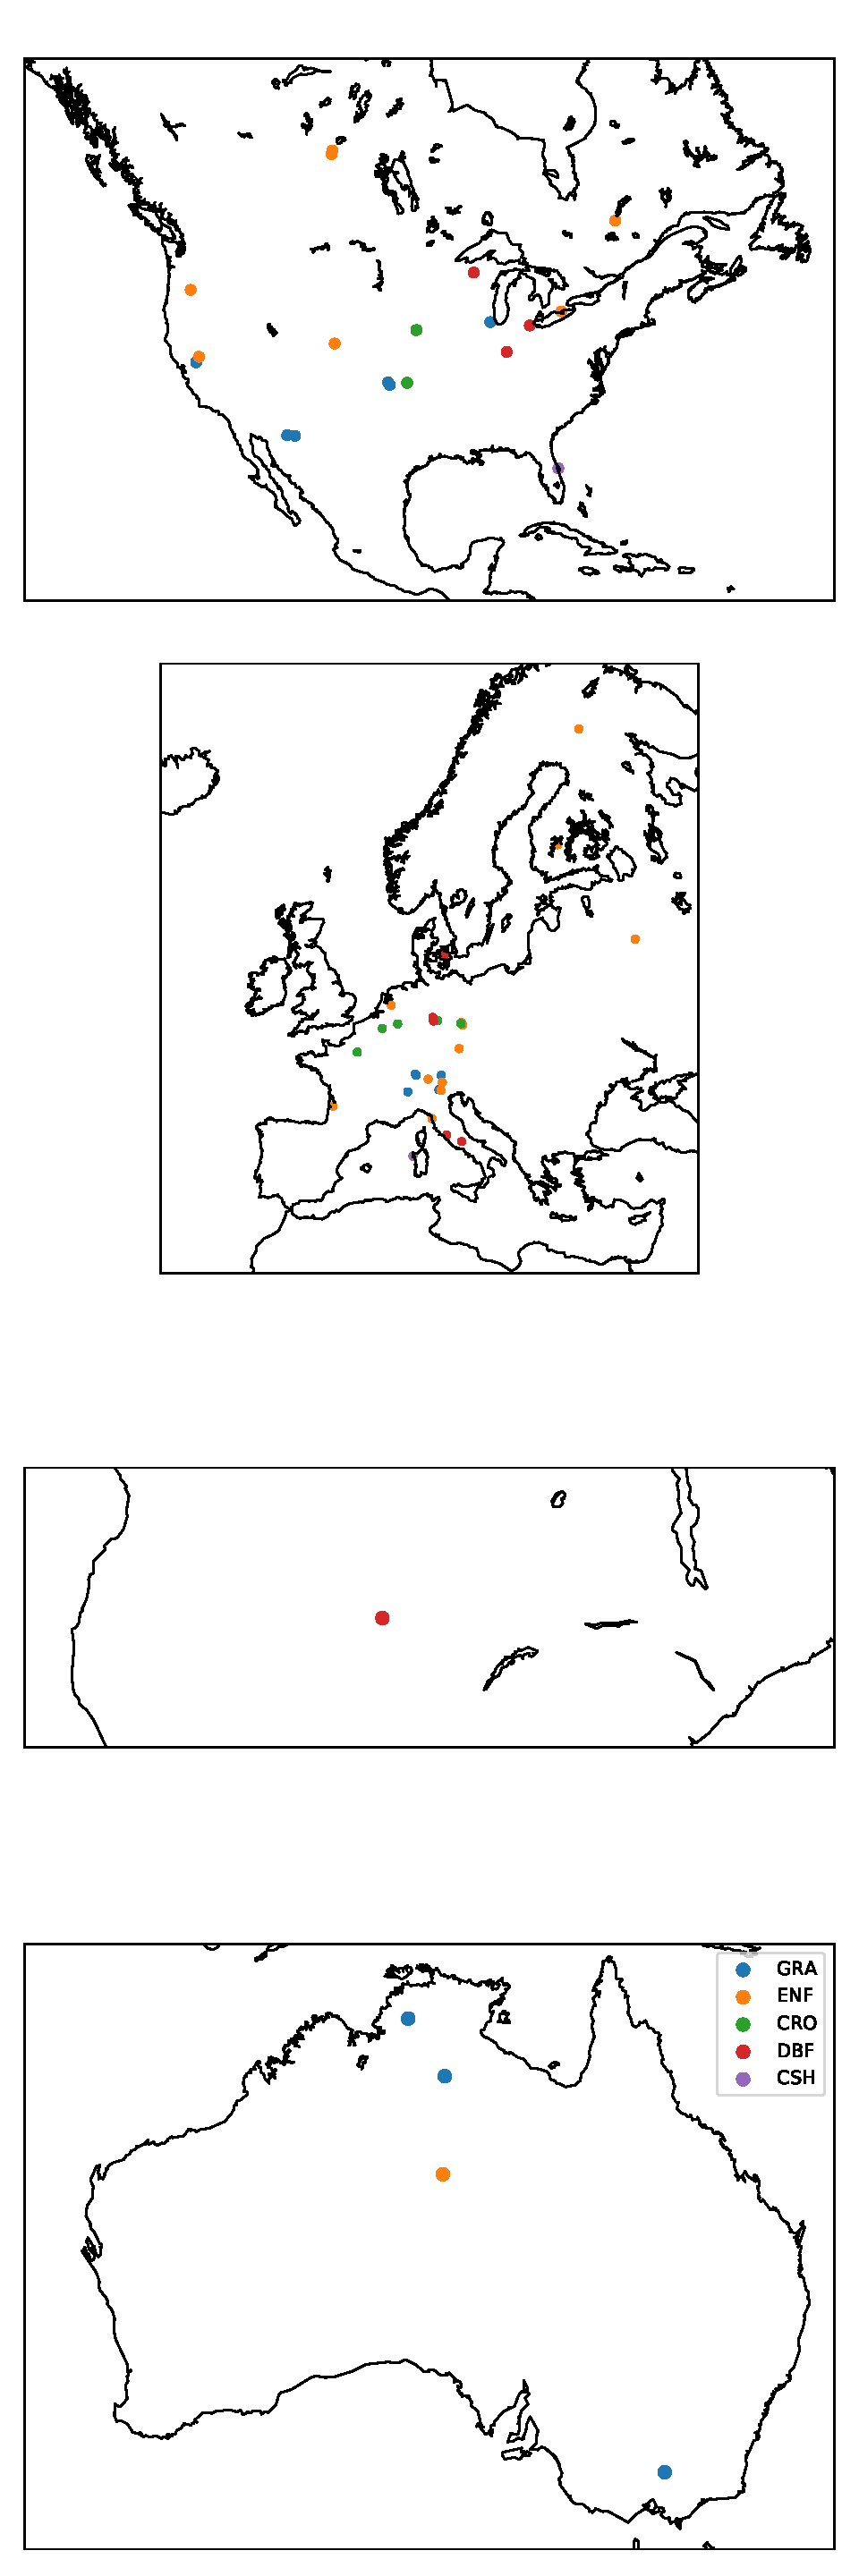
\includegraphics[width=20pc]{./fig01.pdf}
\caption{Plant functional type and location of sites used in analysis. ***\textbf{This is just  a placeholder for now, I am currently fixing it***}}
\label{map_fig}
 \end{figure}

\section{Results}
\label{results}

By construction, the variability in the $\sigma$ term (Equation \ref{sigma}) contains all model and observational uncertainties. For an observation that perfectly matches our model and constant uWUE assumption $\sigma$ will be one. Therefore, for our assumptions and framework to be reasonable $\sigma$ should be $O(1)$. Figure \ref{lai_fig} presents the histogram of calculated $\sigma$s with outliers removed (lowest and highest 5\% percent). All remaining $\sigma$ values are close to unity ($O(1)$) which provides confidence in model framework.

\begin{figure}[h]
\centering
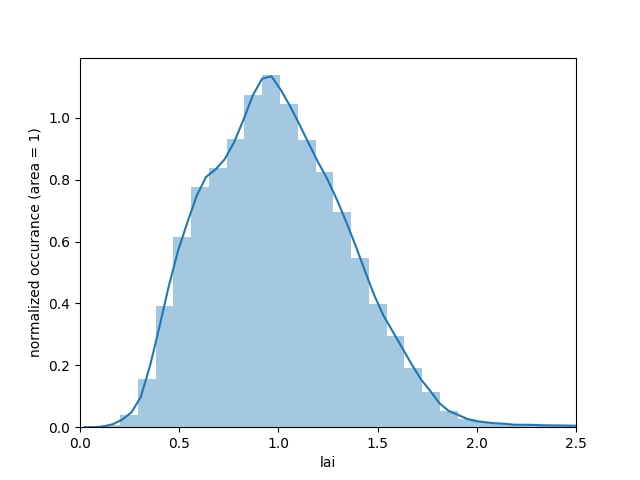
\includegraphics[width=20pc]{./fig02.png}
\caption{Histogram of $\sigma$ values calculated for each site and time according to Equation \ref{sigma}. The lowest and highest 5\% are removed as outliers, as well as any values below 0. The curve is normalized such that its area is 1. }
\label{lai_fig}
\end{figure}

An additional concern is that $\sigma$ may in fact be correlated with $VPD$, in which case the dependence would need to be accounted for when taking the derivative. Figure \ref{lai_vpd_fig} plots the joint distribution of $\sigma$ and VPD, and shows that $\sigma$ is very weakly a function of VPD. Given this weak dependence, we argue that Equation \ref{d_et} is a valid approximation for ET response to $VPD$.

\begin{figure}[h]
\centering
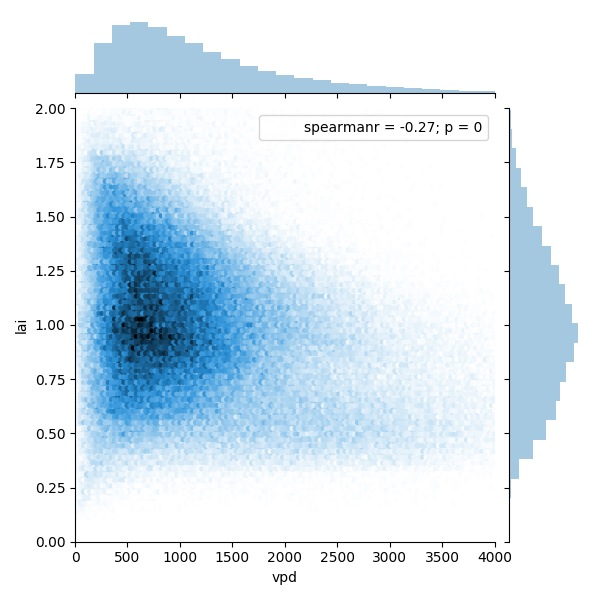
\includegraphics[width=20pc]{./fig03.png}
\caption{The joint distribution of $VPD$ and $\sigma$. $\sigma$ has only a weak dependence on $VPD$. \textbf{***note I am redoing/cleaning up this plot, ``lai'' should read sigma***}}
\label{lai_vpd_fig}
\end{figure}

Before calculating the sensitivity of ET to VPD, we will consider the functional form of Equation \ref{d_et}. There are two main terms: a ``scaling'' term, which modifies the magnitude but not the sign of the derivative $\partial ET/\partial VPD$:

\begin{equation}
  \frac{g_a \; P}{T(\Delta + \gamma)},
\end{equation}

and a ``sign'' term, which determines whether the derivative is positive i.e. atmospheric demand driven or negative i.e. physiologically controlled:

\begin{equation}
  \label{sign}
  \frac{c_p}{R_{air}} - \frac{\gamma c_s }{1.6 \; R\; \text{ uWUE }} \left( \frac{2 g_1 + \sqrt{VPD}}{2 (g_1 + \sqrt{VPD})^2}\right).
\end{equation}
All variables are positive, so the relative magnitude between the first term and the second term in Equation \ref{sign} will determine whether ET increases or decreases with increasing VPD. If the second term is larger magnitude then plant response dominates, while if the first term is larger then atmospheric demand dominates. The sign will determine whether ET is increasing or decreasing and we thus evaluate its functional form first. 

\subsection{Functional Form of the Sign Term}
\label{sign_func}
First, we explore the variables within the sign term to gain better intuition on the driver of either the increase or reduction of ET with VPD. $c_s$ and $\gamma$ are relatively constant to a good approximation so that the variability is dominated by $\sigma$ and $VPD$. $uWUE$ could vary with soil moisture but has been shown to be relatively constant except in very dry soil conditions \citep{Zhou_2016, Lin_2015}. We thus further assume that the soil is not too dry so that $uWUE$ can be approximated as a constant. This then means that the sign term only depends on VPD for a given PFT and is approximately just a function of $VPD$. We can further determine a critical threshold separating an increase from decrease in ET, such that $VPD_{crit}$ where $\frac{\partial \; ET}{\partial \; VPD} = 0$:

\begin{linenomath*}
  \begin{equation}
VPD_{crit} = \frac{R_{air}}{4 c_p} \left( \frac{\gamma c_s}{1.6\; R \; \overline{\sigma} uWUE} + \sqrt{\frac{\gamma c_s}{1.6\; R \; \overline{\sigma} uWUE}\left( \frac{\gamma c_s}{1.6\; R \; \overline{\sigma} uWUE} + 8 g_1 \frac{c_p}{R_{air}}\right)} - 4 g_1 \frac{c_p}{R_{air}} \right)
\label{vpd_min_et}
  \end{equation}
\end{linenomath*}

Values of $VPD_{crit}$ as a function of PFT are shown in Table \ref{vpd_crit}. For any values of $VPD$ less than $VPD_{crit}$, $\frac{\partial \; ET}{\partial \; VPD}$ will be negative, and for values of $VPD$ greater than $VPD_{crit}$, $\frac{\partial \; ET}{\partial \; VPD}$ will be positive. In other words, ecosystems can regulate and mitigate evaporative losses up to a VPD limit, above which atmospheric demand is just too high to be entirely compensated by stomatal regulation. We note however that even though ET increases again above the critical threshold, $VPD_{crit}$, ET is still much lower that potential evaporation as stomata are stills strongly regulating vapor fluxes. Even in the absence of soil pore evaporation, stomata do not shut down entirely at very high VPD and ET does not go to zero, because stomata are still slightly open to perform some photosynthesis \citep{Ball_1987, Leuning_1990, Medlyn_2011}. In addition, upward xylem transport is necessary to maintain phloem transport and thus carbon allocation (MENCUCCINI) \explain{Not sure citation  - Comparative criteria for models of the vasuclar transport systems of tall trees}.

\begin{table}
  \label{vpd_crit}
\caption{Values of $VPD_{crit}$, where $\frac{\partial \; ET}{\partial \; VPD} = 0$, evaluated at PFT average values for $R_{air}$, $\sigma$, $\gamma$, and $c_s$. For reference, these values are also provided CITE TABLE. For values of $VPD$ less than $VPD_{crit}$, $\frac{\partial \; ET}{\partial \; VPD}$ will be negative, and for values of $VPD$ greater than $VPD_{crit}$, $\frac{\partial \; ET}{\partial \; VPD}$ will be positive. \textbf{**** this statistics are dated, need to update***}}
\centering
\begin{tabular}{l c c c c c c}
  \hline
  PFT & $R_{air}$ & $c_s$ (ppm) & $\gamma$ &  uWUE    & \textbf{$VPD_{crit}$ (Pa)} \\
  \hline
  CRO &  288.680920 & 372.567691& 65.351523& 2.602873&  \textbf{133.165438} \\
  CSH &   289.067152& 381.593622& 67.613172& 2.175278& \textbf{4439.564212} \\
  DBF &   288.624437& 377.449849& 63.421812& 2.746393&  \textbf{888.773243} \\
  ENF &  288.183849& 377.676463& 61.559242& 4.015362&  \textbf{978.084845} \\
  GRA &  288.425651& 377.264645& 61.598768& 2.281074& \textbf{1141.630778} \\
\hline
\multicolumn{2}{l}{$^{a}$Footnote text here.}
\end{tabular}
\end{table}

Differences in $uWUE$ and $g_1$ between PFTs alter the functional form of the sign term.  Larger $uWUE$ and $g_1$ will shift the sign term towards overall positive values. $g_1$ additionally plays a primary role in determining dependnece on VPD: the smaller $g_1$, the greater the $VPD$ dependence for the PFT (Figure \ref{term3}).

Based on Figure \ref{term3} and Table \ref{vpd_crit}, CROs are the least water conservative and have the most positive constant offset, while CSH are the most water conservative and have the most negative constant offset in the sign term.  ENF ($g_1 = 74.31$) has by far the largest VPD dependence of response, while CRO ($g_1 = 183.1$) has the smallest VPD dependence. ENF are less willing to trade water for new growth, so the regulate water much more strongly depending on the dryness environment (VPD). CRO on the otherhand are more willing to trade water for new growth, so they regulate water relatively similiarly irregardless of the environment.
 
A primary takeaway from Figure \ref{term3}a is that according to our theory for all PFTs except for crops there is frequent occurrence of a negative (plant dominating) ET response to increases in VPD. This thus means that plants are able in most atmospheric conditions to redue ET in response to increased VPD and thus to reduce water losses. To better illustrate this, the ranges of observed environmental VPDs at the FLUXNET sites are plotted parallel to the x-axis. For CSH, VPD is always less than VPD$_{crit}$ so that the plant response dominates and empathizes the water conservative strategy of those plants. For CRO on the other, VPD is almost always higher than VPD$_{crit}$, emphasizing that those plants are water intensive and were actually engineered for photosynthesis rather than water saving. For forests and grass, whether plant response or atmospheric demand dominates is more dependent on the environment, with about half of of observed VPD less than VPD$_{crit}$, i.e. in conditions where plant response dominates. It is also important to note that even when atmospheric demand dominates, the response is still far smaller than it would be for potential evaporation i.e. atmospheric demand only, emphasizing that there is still a strong regulation of evaporative flux by stomata and though the plant xylem. The sign term in this case would just be a constant ($\frac{c_p}{R_{air}} \approx 3.5$), which is far larger than any part of the curves for any PFT. This highlights the deficiencies of PET's ability to capture land response to changes in atmospheric dryness (VPD). Plants are always regulating water exchange from the land surface, even when they reach the limits of they ability to do so. Therefore, the actual land surface reponse to a change in VPD will always me more negative than if the plants are not included in the physics (PET). However, we have assumed $\sigma$ (uncertainty) equal to one. We still need to test if inclusion of uncertainty could change our conclusions.
\begin{figure}[h]
\centering
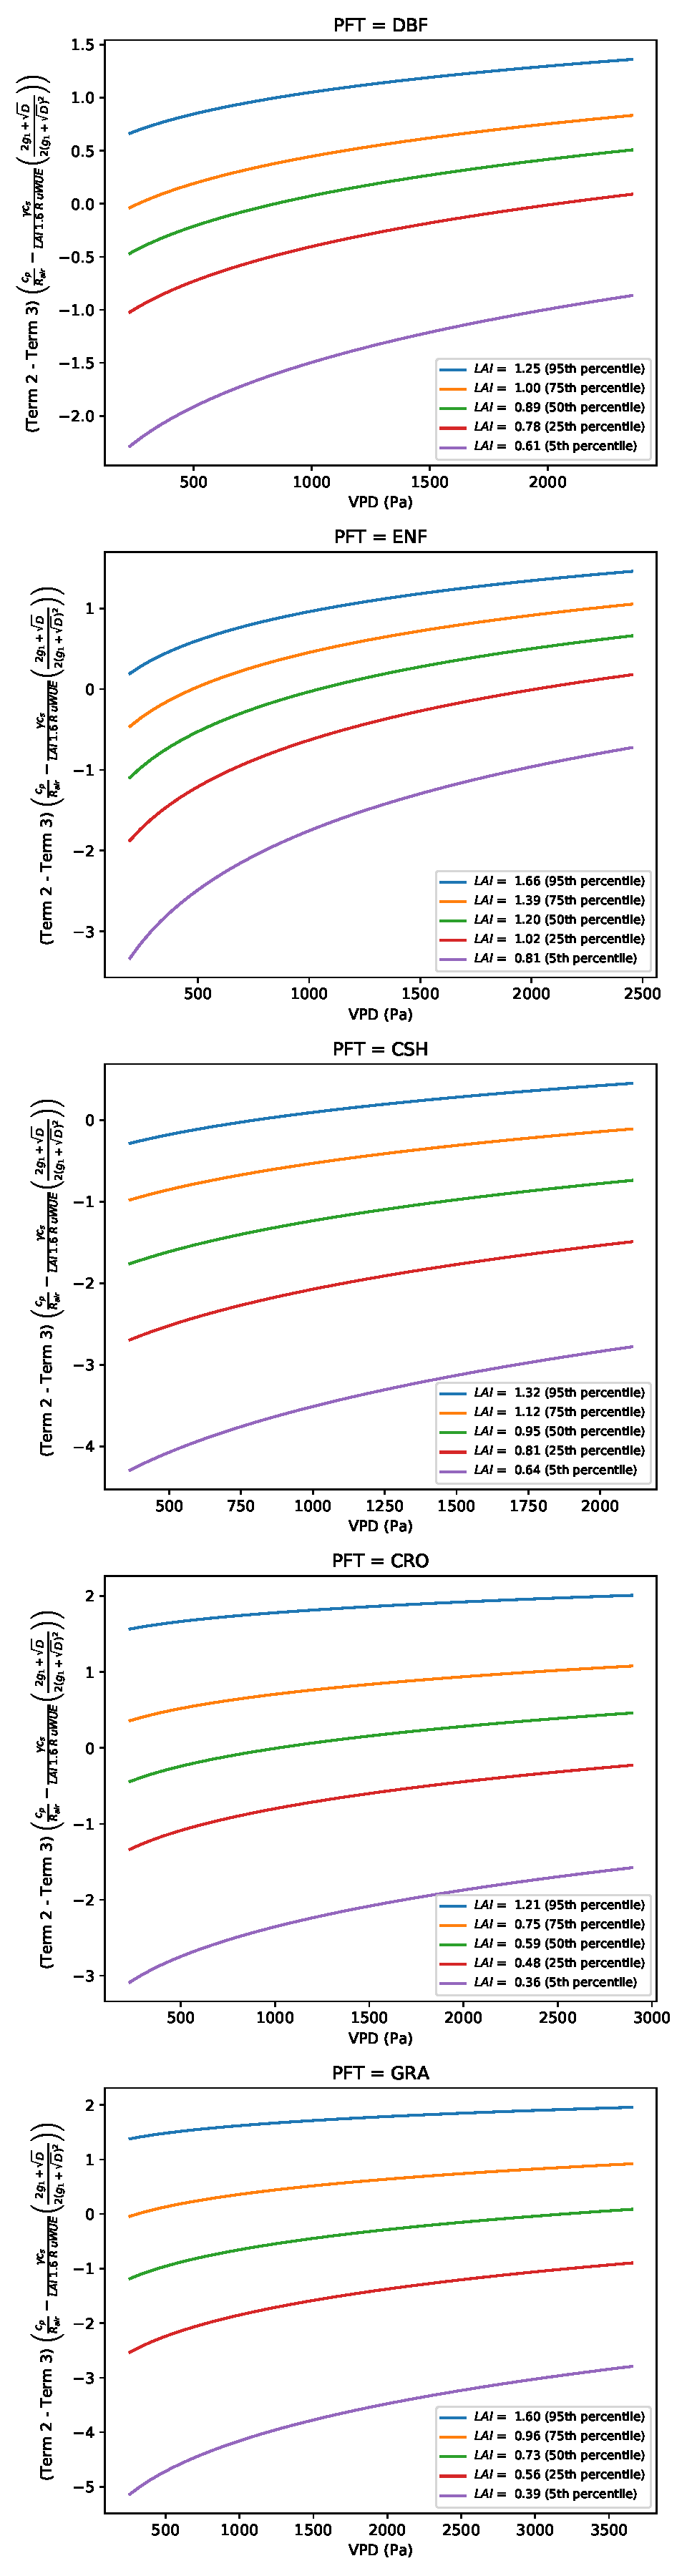
\includegraphics[width=20pc]{./fig05.pdf}
\caption{Sources of variability for the sign term. Top: sign term as a function of VPD, with $\sigma$ held fixed at 1. The observed range of VPD for each PFT is also shown below the x-axis. Line extent corresponds to 5th and 95th percentiles, while stars denote the location of the 25th, 50th, and 75th percentiles.

Bottom: The location of the minima of ET, as a function of VPD and $\sigma$. Lines and stars denote the distribution of VPD and $\sigma$ next to each axis, following the same percentiles as above. \textbf{***need to replot with correct sigma (normalized to 1), also correct uWUE label in first plot***}}
\label{term3}
\end{figure}

Figure \ref{term3}b shows the location of VPD$_{crit}$, as a function of $\sigma$ (uncertainty) and $VPD$. For any $\sigma$ or VPD less (more) than these curves, the sign term will be negative (positive). It is clear that the portion of VPD observations below/above these curves will be a strong function of $\sigma$. This motivates a thorough examination of how inclusion of uncertainty ($\sigma$) might change the form of the sign term, and in particular the location of VPD$_{crit}$ for each of our plant types. In Secion \ref{testing} we examine if and how uncertainty changes the analysis presented in this section, for each PFT.

\subsection{Functional Form of the Scaling Term}

While the above discussion of the sign of $\frac{\partial \; ET}{\partial \; VPD}$ is important to answer our research question, the magnitude of $\frac{\partial \; ET}{\partial \; VPD}$ will also the relative magnitude of the change $\frac{\partial \; ET}{\partial \; VPD}$ and the importance of $VPD$ variability for overall $ET$ variability. So we now more closely examine the scaling term: $\frac{P}{T} \propto \rho$. Air density $\rho$ scaling term varies little relative to aerodynamic conductance and $\Delta$. The psychrometric constant $\gamma$ is also relatively constant, so the scaling term should be primarily a function of aerodynamic conductance and temperature, through the slope of the Clauisu-Clapeyron relationship $\Delta$. This is as expected, given that the aerodynamic conductance represents the efficiency fo the transfer of surface anomalies to the atmosphere. As aerodynamic conductace  increases, any plant response will be communicated more strongly to the atmosphere (and vice-versa).

$\Delta$'s presence in the scaling term also matches physical intuition. Evaporative cooling will dampen the ability of the atmosphere to take more moisture, because $e_{s}$ decreases with decreasing temperature. The decrease in $e_{s}$ is proportional to $\Delta$ ($\delta e_{s} = \Delta \delta T$). So as $\Delta$ increases, you will get a larger damping of ET due to evaporative cooling.  The functional from of $\Delta$ will be the same across PFT, but the temperature range may vary slightly. In contrast, aerodynamic conductance will vary strongly with PFT due to the importance of surface roughness. So most of the differences in scaling between PFT should be in the aerodynamic conductance term. One interesting side note is that the coefficient of variability for both aerodynamic conductance and the scaling term is relatively constant across PFT, suggesting that the influence of aerodynamic conductance on the relative (to the PFT mean) variability of the scaling term is approximately similar across PFT.

Figure \ref{scale_vary}A shows the scaling term normalized by mean aerodynamic conductance (calculated for each plant functional type), and confirms that much of the relative variability of the scaling term is caused by aerodynamic conductance variability. Generally, temperature (via $\Delta$) causes less relative variability. However, the impact of $T$ on the relative variability increases with increasing aerodynamic conductance. 

While the relative variability of scaling term is similar across PFT, the absolute value of scaling term varies strongly across PFT. Figure \ref{scale_vary}B shows scaling term evaluated at the mean aerodynamic conductance for each PFT, and at the range of observed temperatures for each PFT. As expected, for the tree PFTs (DBF, ENF) the scaling term is much larger and the temperature dependence is much stronger. Systematic differences in observed temperatures also cause differences in the average magnitude of scaling term. For example, ENF experiences on average colder temperatures and is thus more likely to have a larger scaling term. Additionally, because the variability of aerodynamic conductance increases proportionally to the mean, the spread of the scaling term due to aerodynamic conductance variability will be larger for the tree PFTs, although this is not shown for simplicity. To summarize Figure \ref{scale_vary}: the variability of the scaling term within each PFT will look like Figure \ref{scale_vary}A for each PFT, but the scale of the y-axis will increase or decrease according to mean aerodynamic conductance observed in Figure \ref{scale_vary}B.
 
\begin{figure}[h]
\centering
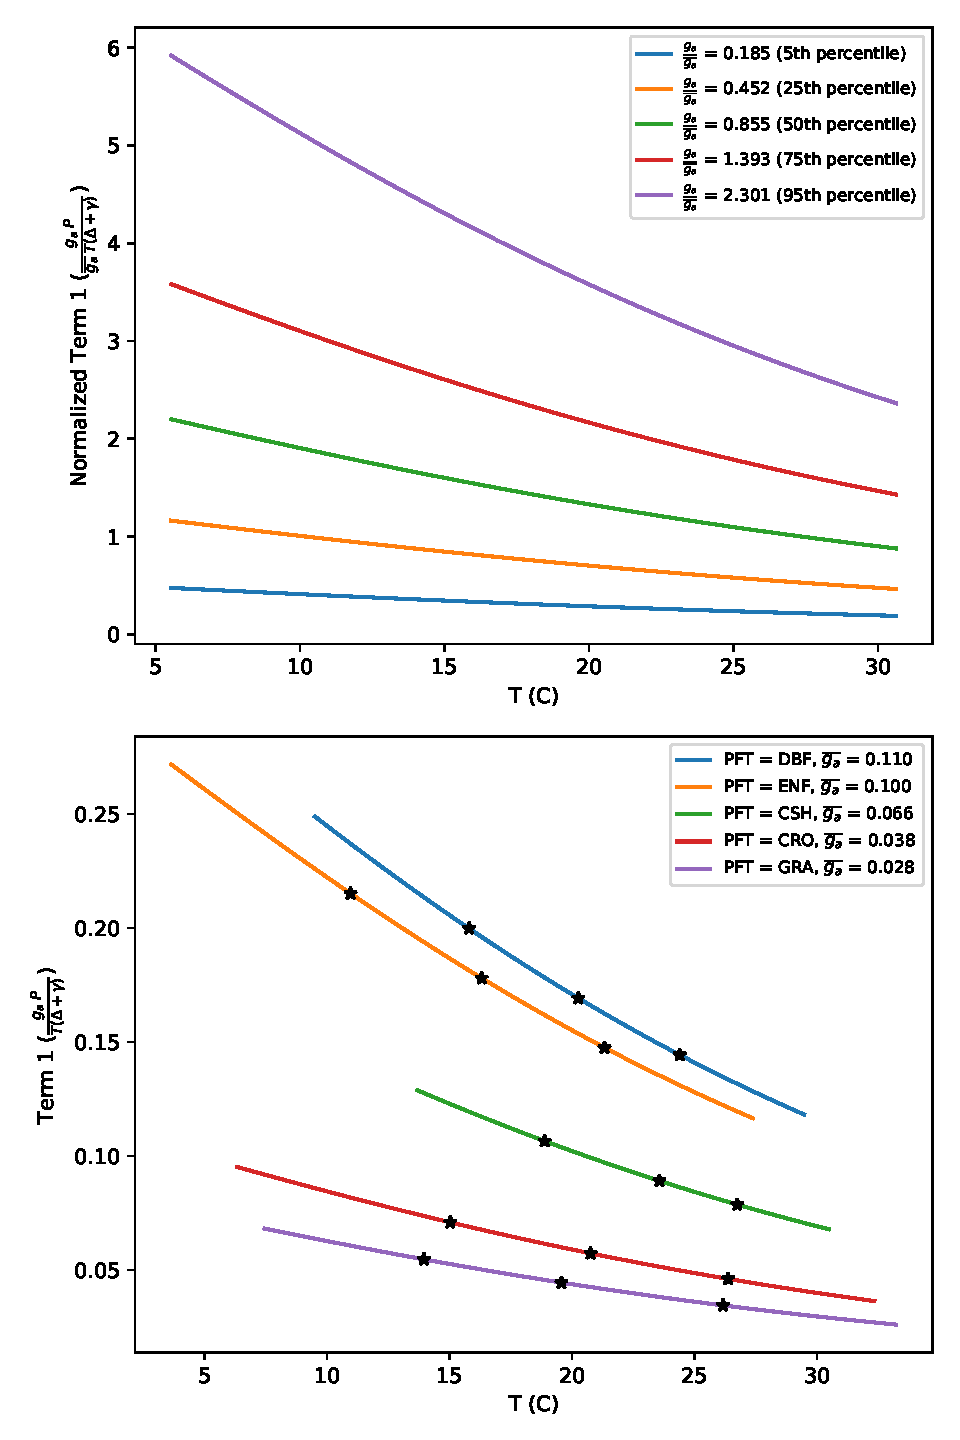
\includegraphics[width=20pc]{./fig04.pdf}
\caption{Primary sources of variability for scaling term. A) Variability within each PFT: scaling term normalized by mean $g_a$ for each PFT. B) Variability between each PFT: scaling term evaluated at mean $g_a$ for each PFT. Temperature range is 5-95th percentile for each PFT. Additionally, stars denote the location of the 25th, 50th, and 75th percentiles.}
\label{scale_vary}
\end{figure}

%%%%% replace below with idea:
\subsection{Bulk statistics of $\frac{\partial \; ET}{\partial \; VPD}$}

Table 3 confirms our expectations for PFT behavior of $\frac{\partial \; ET}{\partial \; VPD}$. For all PFTs except for CRO, average $\frac{\partial \; ET}{\partial \; VPD}$ is less than zero. However, $\frac{\partial \; ET}{\partial \; VPD}$ evaluated at the average of all variables (e.g. $\sigma$, $T$, $c_s$, $VPD$) is only negative for CSH and GRA. And, DBF in addition to CRO experiences $\frac{\partial \; ET}{\partial \; VPD}$ < 0 less than half the time. These observations highlight the effect of the nonlinear function in Figure \ref{term3}: $\frac{\partial \; ET}{\partial \; VPD}$ has a much steeper slope when the function is negative, and is thus more likely to be large magnitude.

The units of $\frac{\partial \; ET}{\partial \; VPD}$ make it difficult to interpret if $VPD$ is even a meaningful contributor to ET's variability. To better understand $VPD$'s contribution, we multiply $\frac{\partial \; ET}{\partial \; VPD}\left(\overline{env}\right)$ with $VPD$'s standard deviation to define a (linearized) relative change in ET for variations in $VPD$ . $VPD$'s contribution to ET's variability ranges between 30 - 40 W m$^{-2}$ for all PFTs except for CSH, which is about 100 W m$^{-2}$. Another meaningful comparison is to $\frac{\partial \; ET}{\partial \; R} \cdot std(R)$, as net radiation is generally the driver of ET (cite joe berry here)\explain{Find citation?}. For all PFTs except for CSH $VPD$ contributes between 30 - 40 \% of $R$'s contribution to variability. For CSH the portion is much larger, about 88 \%. $VPD$'s variability is certainly a non-negligible contributor to $ET$'s variability.

Theoretical derivation has so far illuminated the dependence of $\frac{\partial \; ET}{\partial \; VPD}$ and how it varies across PFT. Large mean $uWUE$ shifts CRO and DBF towards a tendancy to increase ET with VPD (positive $\frac{\partial \; ET}{\partial \; VPD}$), but a lower slope parameter ($g_1$) for DBF allows for decreaes in ET with VPD, at low environmental VPD. \explain{physically state how slope parameter is trade for water at leaf level, but uWUE is trade-ff between GPP and VPD at ecosystem-level}.  ENF's very low slope parameter ($g_1$), which is even lower than for DBF, increases the dependence of ET response  ($\frac{\partial \; ET}{\partial \; VPD}$) on $VPD$, and makes the function strongly nonlinear. This has the effect of making mean ET response ($\overline{\frac{\partial \; ET}{\partial \; VPD}}$)  more negative for a given frequency of occurence of negative ET response ($\frac{\partial \; ET}{\partial \; VPD} < 0$), than for other PFT. GRA shows the opposite behavior; a relatively high slope parameter ($g_1$)  makes the function more linear, causing a more positive mean ET reponse ($\overline{\frac{\partial \; ET}{\partial \; VPD}}$) for a given given frequence of negative ET reponse  ($\frac{\partial \; ET}{\partial \; VPD} < 0$). Finally, CSH's very low $uWUE$ dominates the slope parameter's effects, causing ET to almost always decrees with increasing atmospheric dryness (VPD), even with uncertainty included. Variability in $VPD$ accounts for the largest amount of $ET$ variability for CSH. For the other PFTs, $VPD$ contributes less to $ET$ variability, but still represents about 30-40 \% of $R$'s contributions to ET variability. \explain{think pierre is correct, could probably scrap this anecdote: WHAT IS THE SORUCE OF VARIBILITY OF THE REST OF ET I DON"T KNOW IF THAT IS RELEVANT FOR THE PRESENT PAPER.}

\begin{table}
\caption{Statistics of $\frac{\partial \; ET}{\partial \; VPD}$ as a function of PFT. \textbf{***dated, need to update these statistics***}}
\centering
\begin{tabular}{l c c c c c}
  \hline
PFT & $\overline{\frac{\partial \; ET}{\partial \; VPD}}$ & $\frac{\partial \; ET}{\partial \; VPD}\left(\overline{env}\right)$ & $\frac{\partial \; ET}{\partial \; VPD}\left(\overline{env}\right)*\text{std}(VPD)$ & $\frac{\frac{\partial \; ET}{\partial \; VPD}\left(\overline{env}\right)*\text{std}(VPD)}{ \frac{\partial \; ET}{\partial \; R}\left(\overline{env}\right)*\text{std}(R)}$ & fraction $\frac{\partial \; ET}{\partial \; VPD} < 0.$ \\
  \hline
CRO & 0.000853 & 0.026241 & 37.05 & 0.41 & 0.473311\\
CSH & -0.108234 & -0.091526 & 101.72 & 0.88 & 0.931660\\
DBF & -0.012727 & 0.013794 & 39.47 & 0.33 & 0.461674\\
ENF & -0.034087 & 0.000706 & 33.22 & 0.30 & 0.534425\\
GRA & -0.019637 & -0.000921 & 33.60 & 0.35 & 0.631735\\
\hline
  
\end{tabular}
\end{table}


\subsection{Validation of theory at eddy-covariance sites}
\label{testing}
So far we have developed a theory for $\frac{\partial \; ET}{\partial \; VPD}$'s behavior as a function of VPD and PFTs. We now turn to an direct evaluation against observations taken from a wide range of eddy-covariance datasets (Section \ref{methods}).

Figure \ref{agu_fig} shows the distribution of of the sign term (when uncertainty is included), as compared to what the theory would predict. Our goal was to capture the leading order behavior of the ET dependence on VPD. Given the assumptions we have made, and the uncertainties of flux tower observations themselves, we expect a large amount of noise when reprdrocuing the derivatives of ET.

For DBF our theory is successful towards this goal: the theory matches the leading order behavior of the function when uncertainty is included, and the DBG figure looks as one would expect if one just added noise on top of our theory. The VPD dependence, given by the slope parameter ($g_1$), floows the median values of each box plot. Perhaps most importantly, the x-intercept, and thus VPD$_{crit}$, matches nearly exactly between the theory and the observations. Therefor the sign of the ET response to increases in VPD should be well matched, subject to the unavoidable constraints of noise, much of which may be from the observations themselves. The uncertainty is non negligable; there are bany observations in each box for which the the sign of observation is opposite the response predicted by the theory, but to leading order our theory matches the observations. 

While CSH has a much different functional form of the sign term than DBF, CSH observations also match our theory to leading order. Again, the VPD dependence mostly determined from the slope parameter ($g_1$) closely matches the medians in the observation bins. The VPD-independent, strongly negative response, which is determined by $uWUE$, is also captured. For CSH, there is extremely rare occurence of positive ET response with VPD, even with uncertainty, so the sign of the theory almost always matches the sign of the observations, even with all of the uncertainty.

The theory does not match as well for CRO as for DBF and CSH. At low VPD the VPD dependence (due to $g_1$) is similiar to the leading order behavior of the observations, but the entire curve is shifted towards postiive values, due to some error in $uWUE$. Most strikingly, the observations show a tendency to move back towards negative values at high VPD, which given the functional form of VPD dependnce, is behavior that is impossible fo the theory to capture. This divergence between the theory and the observations for CRO could have been expected. For practical reasons, our theory does not include important sources of variability (particularly between sites) for CRO. We do not account for seasonal changes in LAI, variability in crop height and surface roughness, differences in C3 vs C4 photosynthesis, or differences in irrigation practices between the sites and/or years. This deficiencies would explain the inability of our theory to match obsercations. For example, a superpositions of sites with C3 plants (low VPD) and C4 plants (high VPD) would explain observed shift back towards negative ET reponse at high VPD when all sites are binned together, as in Figure \ref{agu_fig}.   

The theory for GRA suffers from similiar limitations as for CRO. The differences between the theory and the observations are more pronounced for GRA, but are explainable using similiar logic as that used for CRO. GRA will also have differences between sites in C3 vs C4 photosythesis, and irrigation practices, as well as strong seasonal variability in crop height and LAI. For GRA, the observations show a very different VPD dependence of response than the theory, with a strong tendency back toewards a negative ET reponse at high VPD which our theory cannot account for. As with CRO, this could be explained by a superposition of sites with C3 vs C4 sites. Unfortunately, because detailed site-level data of C3 vs C4 plant type, as well as irrigation practes, was difficult to obtain, we could not bin GRO and GRA further by irrigation and photosyethesis stragtegy. However, we hypothesize that the theory would much more closel match obsercations with photosythesis and irrigation are accounted for. 

The comparison between the theory and obsercations for ENF is unique from the rest of the PFTs. The VPD dependence of the theory, determined by the slope paramter, is not well captured by observations. However, the theory closely captures the x-intercept and VPD$_{crit}$. So, the theory still captures when the ET reponse will be positive or negative, but is less accurate with the magnitude of the reponse. Therefor the theory is still useful for addressing when VPD drives or reduces ET. Also, it's with noting that we used published constants for $g_1$ \citep[from ][]{Lin_2015}, which determines the VPD dependence. We could have fit our own constants so that the theory would best match the observations, but our goal was to use a priori physical constants whenever possible.

While the above discussion shows that our theory has some limitations when applied to some sites, especially for crops and grasslands, another question could be, how would using PET, as many hydrometeorological studies and applications do, compare with our theory.  Again, as in Section \ref{sign_func}, the PET response to changes in VPD will be constant at about 3.5. In Figure \ref{agu_fig} the ET reponse to shifts in dryness is always far more negative than 3.5 for the observations, even with all uncertainty included. So the PET reponse to atmospheric dryness is outside the range of all observable responses. This casts doubt on PET's usefulness for capturing the leading order behavior of water budgeting at the land surface. However our theory (Equation \ref{et}) could be used with published $uWUE$ and $g1$ as an alternative to PET to estimating land response and moisture budgeting.

\subsubsection{Testing VPD$_{crit}$}
As stated in the above discussion of ENF, we are mostly interested in the critical threshold $VPD_{crit}$ for which the sign of  $\frac{\partial \; ET}{\partial \; VPD}$ is determined. When $VPD < VPD_{crit}$, $\frac{\partial \; ET}{\partial \; VPD}  < 0$ (plant response dominates), and when $VPD > VPD_{crit}$, $\frac{\partial \; ET}{\partial \; VPD} > 0$ (atmospheric demand dominates). Theoretically this $VPD_{crit}$ is only a function of PFT. We can look at how this value of $VPD_{crit}$ matches the data as different observed variables (including uncertainty) are allowed to vary.


Figure \ref{real} presents calculated $\frac{\partial \; ET}{\partial \; VPD}$ where, unless otherwise noted, all variables in Equation \ref{d_et} are allowed to vary, including uncertainty. Each column represents a different quantity related to $\frac{\partial \; ET}{\partial \; VPD}$, and each row is a different PFT. Vertical black lines denote where our theory says $VPD_{crit}$ should be. For any observations to the left of this line $\frac{\partial \; ET}{\partial \; VPD}$ should be negative (plant response dominates), and any observations the right of the line should be positive (atmospheric demand dominates). In addition to seeing how our theoretically-derived VPD threshold, $VPD_{crit}$, matches observations, these analysis are also useful for observing how the scaling term affects the magnitude of the derivative, if at all. 

The scatter figures generally confirm expectations from Figure \ref{agu_fig}. By comparing different columns of Figure \ref{real} we can evaluate the impact of $\sigma$ and $g_a$ on the variability of $\frac{\partial \; ET}{\partial \; VPD}$. $g_a$'s scaling (included in columns 1 and 3) alters the magnitude considerably, particularly between PFTs. $\sigma$ variability (included in columns 1 and 2) adds a lot of additional noise to the signal of $\frac{\partial \; ET}{\partial \; VPD}$, as observed in Figure \ref{agu_fig}. However, the general story with the noise appears to match the cleaner signal when $\sigma$ is help constant and $VPD_{crit}$ is clearly visible. The exceptions are, as discussed above, for GRA and CRO, where the full complexity plots (Columns 1 and 2) do not match well with $\sigma$ held fixed (Columns 3 and 4).

While $g_a$ has a large impact on the magnitude of the scaling, temperature, through the derisive of the Clausius-Clapeyron, $\Delta$, term, does not appear to have as much of an impact in the complete estimation of $\frac{\partial \; ET}{\partial \; VPD}$. Therefore it appears that the absolute magnitude of the derivative can be mostly attributed to the sign term, and its direct scaling by aerodynamic conductance. Intuitively this is reasonable; aerodynamic conductance will control how dominant balances at the land surface are communicated to the boundary layer. While $\Delta$ controls the efficiency of latent fluxes in carrying heat away from the surface, it appears this is a second order term, relative to $g_a$, for scaling $\frac{\partial \; ET}{\partial \; VPD}$. 

In general Figures \ref{real} and \ref{agu_fig} match our expectations, even with the large sensitivity to $\sigma$ seen in Figure \ref{term3}. Our $\sigma$-based method of uncertainty propagation blurs the idealized expectations the most for GRA and CRO. We therefore have the most confidence in our conclusion based on Equation \ref{d_et} for PFTs CSH, DBF, and ENF, as the sign of the derivative with uncertainty included matches (to leading order) the story when $\sigma$ is held fixed.

\begin{figure}[h]
\centering
\includegraphics[width=\textwidth]{./agu_fig.pdf}
\caption{Comparison of the sign term with model uncertainty included (box plots) to the sign term as calculated with simplifying assumptions (blue line).}
\label{agu_fig}
\end{figure}


\begin{figure}[h]
\centering
\centerline{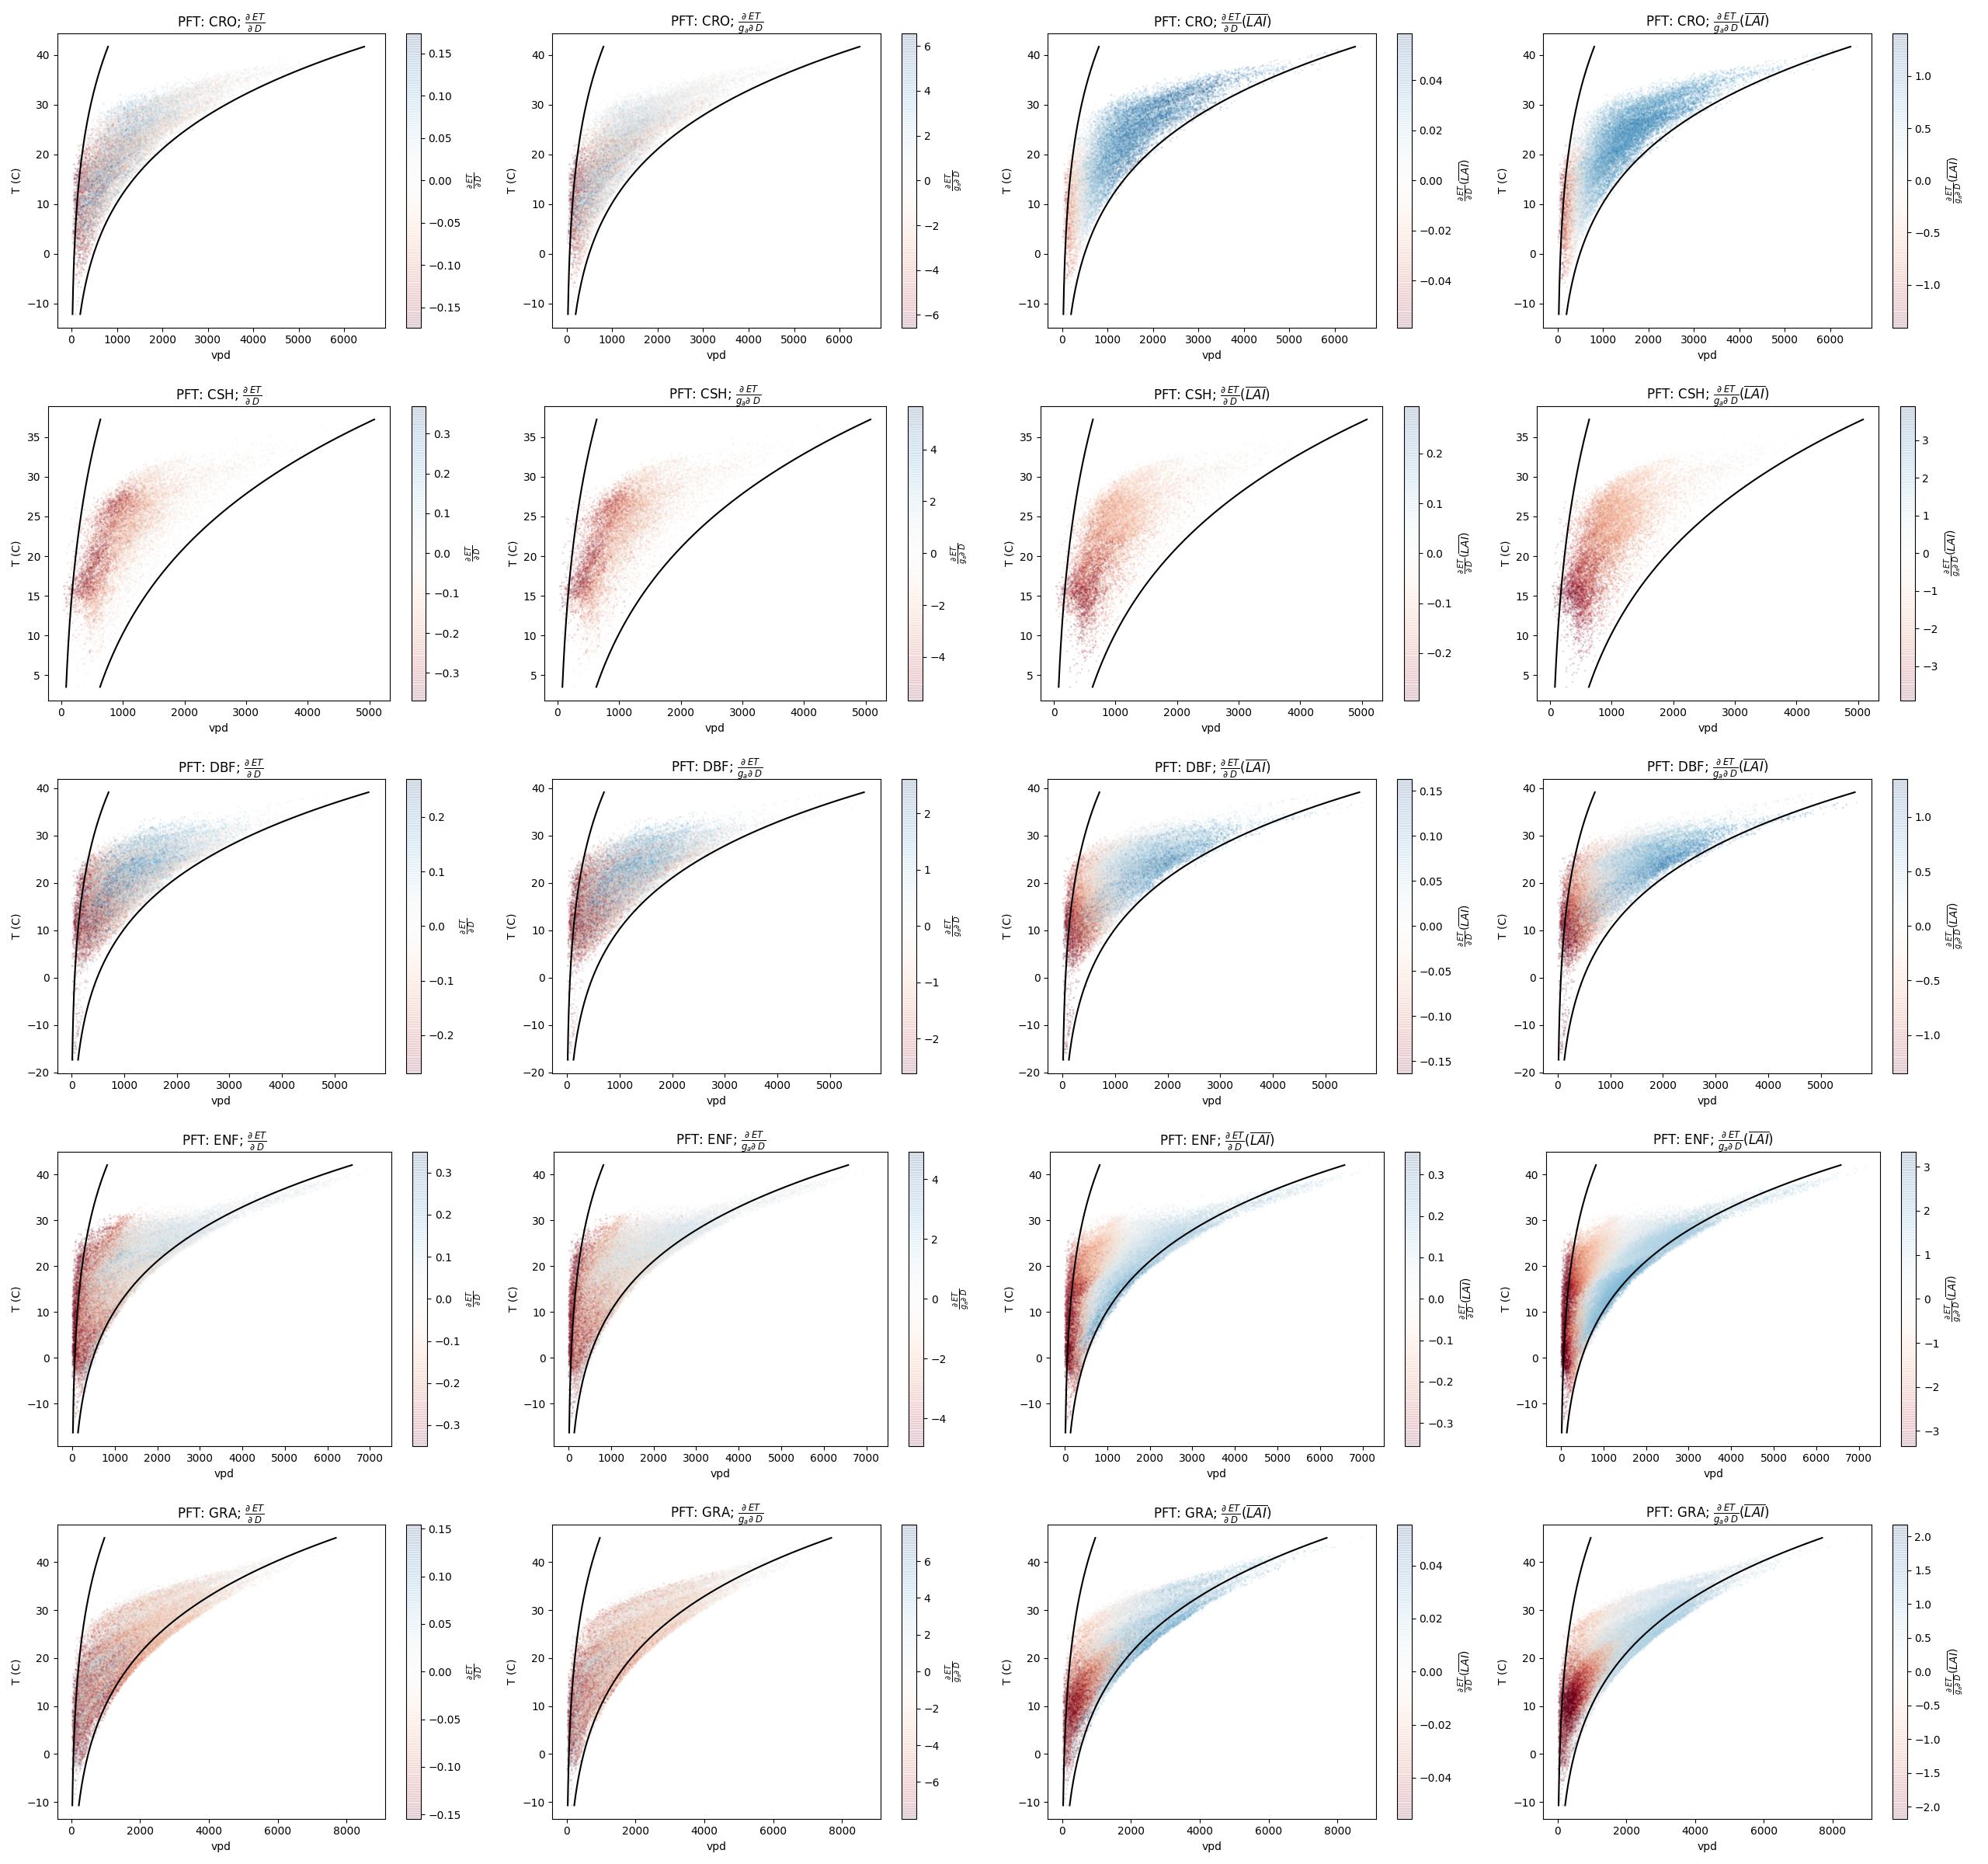
\includegraphics[width=1.4\textwidth]{./fig06.png}}
\caption{Scatter plots of $\frac{\partial \; ET}{\partial \; VPD}$. Each row is a different PFT, and each column is a different quantity related to $\frac{\partial \; ET}{\partial \; VPD}$, as labeled: Column 1: $\frac{\partial \; ET}{\partial \; VPD}$; Column 2: $\frac{\partial \; ET}{\partial \; VPD}$ normalized by $g_a$; Column 3: $\frac{\partial \; ET}{\partial \; VPD}$ with $\sigma$ held fixed at 1; and Column 4: $\frac{\partial \; ET}{\partial \; VPD}$ normalized by $g_a$ and with $\sigma$ held fixed. Please note differences in the colorbar scale.}
\label{real}
\end{figure}

% \begin{figure}[h]
% \centering
% 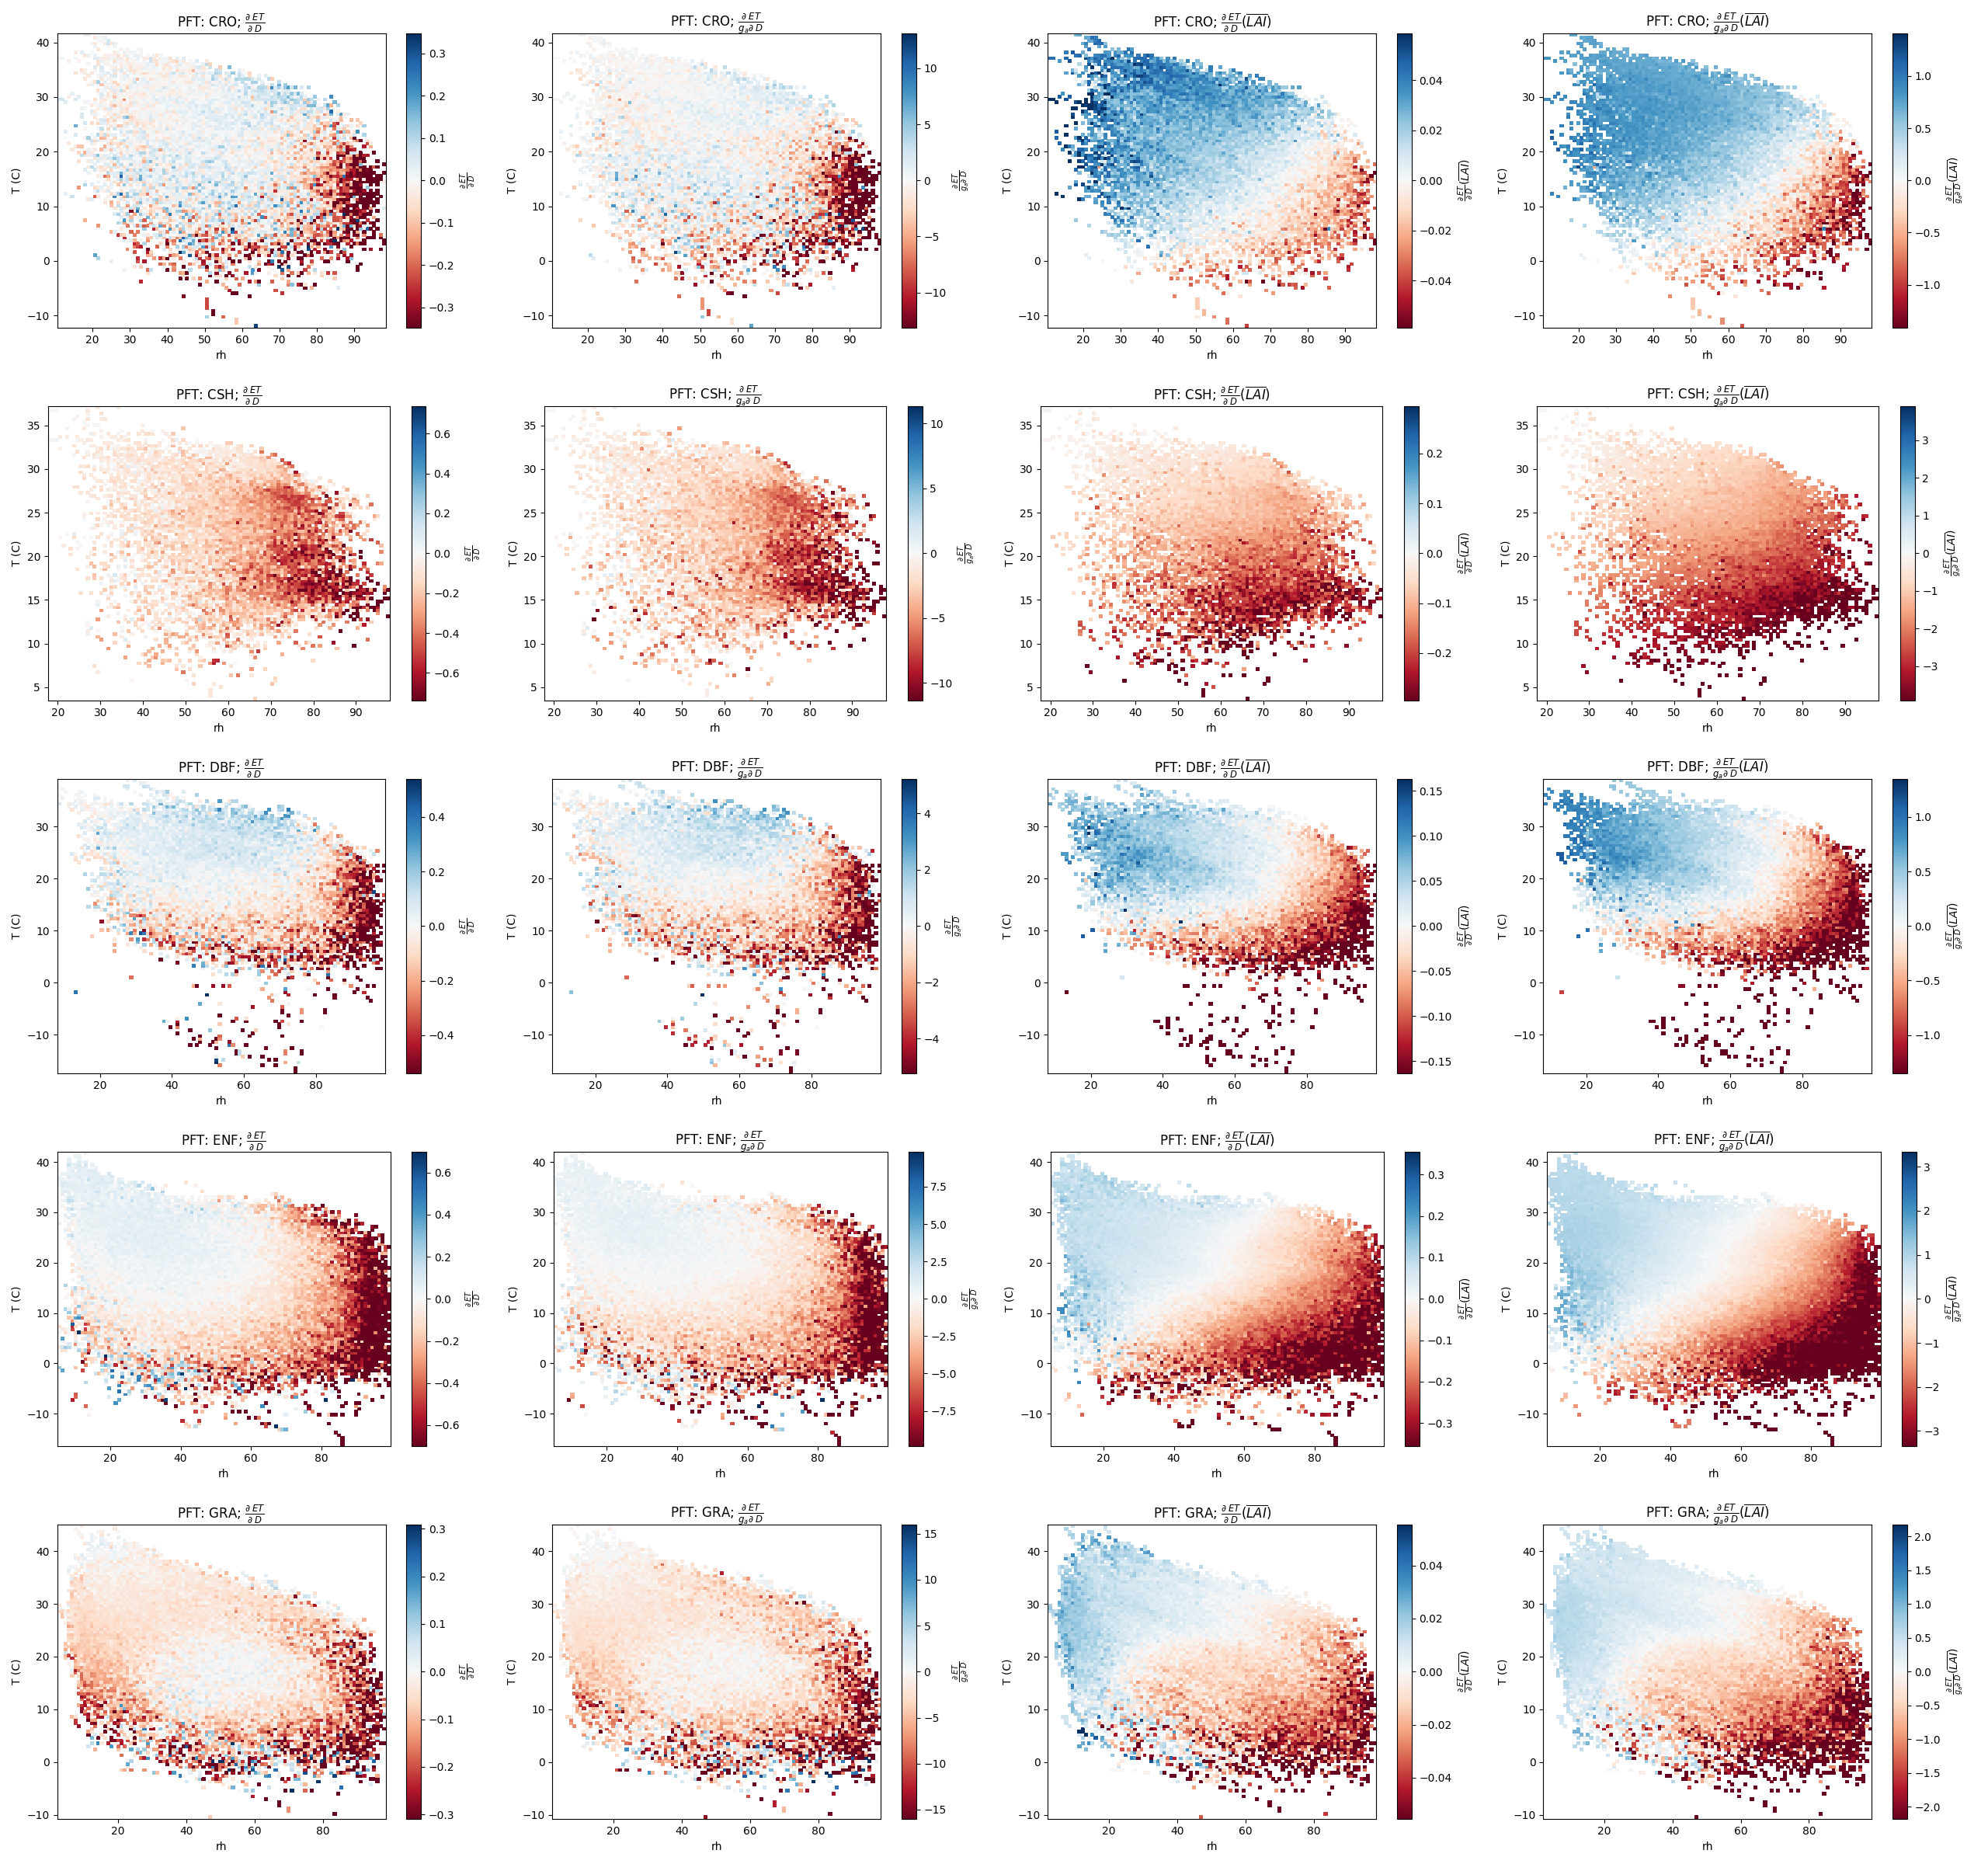
\includegraphics[width=\textwidth]{./fig06b.png}
% \caption{****alternate Fig 06****  Scatter plots of $\frac{\partial \; ET}{\partial \; VPD}$. Each row is a different PFT, and each column is a different quantity related to $\frac{\partial \; ET}{\partial \; VPD}$, as labeled. If I end up using this, I could also draw on the curve of $VPD_{crit}$ with $\overline{\frac{\text{LAI}}{\text{LAI$_{ref}$}}}$. }
% \label{real2}
% \end{figure}


\section{Limitations of theory}
\explain{HERE DISCUSS LIMITATION OF THE METHODS TO BVERY DRY CONDITIONS AND THE FEEDBCAK TO THE ATMOSPHERE OF VERY DRY SOIL CONDITIONS (BERG ET AL 2016, GENTINE ET AL> 2016)}

\section{Conclusions} 

We derived a new form of Penman Monteith using $uWUE$ (\cite{Zhou_2015}) to remove the stomatal conductance term's implicit dependence on ET. With our new form of Penman Monteith we developed a theory for when an ecosystem will tend to reduce or increase ET with increasing VPD. The goal was to capture the leading order behavior of the system to gain some intrinsic knowledge for its behavior. This intuition can be used to disentangle land atmosphere feedbacks in more complicated scenarios, and will aid interpretation of observations and sophisticated models.

Our theory states that each plant type has a critical VPD below which ET will decrease (plant response dominating) and above which ET will increase (atmospheric demand dominates). We tested our theory using data from FLUXNET 2015, and found that for DBF and CSH the theory succeeds in capturing the leading order behavior. For ENF, the theory succeeds in capturing the leading order behavior for the sign of $\frac{\partial \; ET}{\partial \; VPD}$, but not for magnitude. In contrast, the model does not capture the behavior for CRO and GRA. In some ways we should have expected this, as our theory does not account for large sources of variability we would expect for those plant types, including varying surface roughness, c3 vs c4 photosynthesis, and potential differences in irrigation across sites. Given these deficiencies for CRO and GRA, we will withhold conclusions on their response to increasing VPD.

For the forest sites (DBF, ENF) the observed environmental VPD approximately straddles the critical VPD, with about half the observations below the critical VPD and half above. However for CSH the environmental VPD never exceeds the critical VPD, and even when uncertainty is included the sign of the derivative is almost always negative (93\% of observations).

While our theory predicts common occurrence of positive $\frac{\partial \; ET}{\partial \; VPD}$ (atmospheric demand dominates), the plant response is still important even when $\frac{\partial \; ET}{\partial \; VPD} > 0$. The magnitude of the ``sign term'' of our theory is always far below what it would be if we only considered the atmospheric demand term (PET). This means that any drought indices or analysis using PET will not capture how the vegetated surface respond and react to increases in atmospheric demand. However, the new uWUE-version of Penman Monteith we derived (Equation \ref{et}) could be used as a complement to PET in drought indices. One could calculate and compare indices  when plant response is ignored (PET) or included (Equation \ref{et}). 

This paper provides initial intuition for how the land surface responds to atmospheric drying. This intuition for the one-way behavior of  land surface response to atmospheric drying is critical first step to disentangling land-atmosphere feedbacks at various scales, from diurnal to seasonal and beyond. 

%%
%% Enter Figures and Tables near as possible to where they are first mentioned:
%
% DO NOT USE \psfrag or \subfigure commands.
%
% Figure captions go below the figure.
% Table titles go above tables;  other caption information
%  should be placed in last line of the table, using
% \multicolumn2l{$^a$ This is a table note.}
%
%----------------
% EXAMPLE FIGURE
%
% \begin{figure}[h]
% \centering
% when using pdflatex, use pdf file:
% \includegraphics[width=20pc]{figsamp.pdf}
%
% when using dvips, use .eps file:
% \includegraphics[width=20pc]{figsamp.eps}
%
% \caption{Short caption}
% \label{figone}
%  \end{figure}
%
% ---------------
% EXAMPLE TABLE
%
% \begin{table}
% \caption{Time of the Transition Between Phase 1 and Phase 2$^{a}$}
% \centering
% \begin{tabular}{l c}
% \hline
%  Run  & Time (min)  \\
% \hline
%   $l1$  & 260   \\
%   $l2$  & 300   \\
%   $l3$  & 340   \\
%   $h1$  & 270   \\
%   $h2$  & 250   \\
%   $h3$  & 380   \\
%   $r1$  & 370   \\
%   $r2$  & 390   \\
% \hline
% \multicolumn{2}{l}{$^{a}$Footnote text here.}
% \end{tabular}
% \end{table}

%% SIDEWAYS FIGURE and TABLE 
% AGU prefers the use of {sidewaystable} over {landscapetable} as it causes fewer problems.
%
% \begin{sidewaysfigure}
% \includegraphics[width=20pc]{figsamp}
% \caption{caption here}
% \label{newfig}
% \end{sidewaysfigure}
% 
%  \begin{sidewaystable}
%  \caption{Caption here}
% \label{tab:signif_gap_clos}
%  \begin{tabular}{ccc}
% one&two&three\\
% four&five&six
%  \end{tabular}
%  \end{sidewaystable}

%% If using numbered lines, please surround equations with \begin{linenomath*}...\end{linenomath*}
%\begin{linenomath*}
%\begin{equation}
%y|{f} \sim g(m, \sigma),
%\end{equation}
%\end{linenomath*}

%%% End of body of article

%%%%%%%%%%%%%%%%%%%%%%%%%%%%%%%%
%% Optional Appendix goes here
%
% The \appendix command resets counters and redefines section heads
%
% After typing \appendix
%
%\section{Here Is Appendix Title}
% will show
% A: Here Is Appendix Title
%
%\appendix
%\section{Here is a sample appendix}

%%%%%%%%%%%%%%%%%%%%%%%%%%%%%%%%%%%%%%%%%%%%%%%%%%%%%%%%%%%%%%%%
%
% Optional Glossary, Notation or Acronym section goes here:
%
%%%%%%%%%%%%%%  
% Glossary is only allowed in Reviews of Geophysics
%  \begin{glossary}
%  \term{Term}
%   Term Definition here
%  \term{Term}
%   Term Definition here
%  \term{Term}
%   Term Definition here
%  \end{glossary}

%
%%%%%%%%%%%%%%
% Acronyms
%   \begin{acronyms}
%   \acro{Acronym}
%   Definition here
%   \acro{EMOS}
%   Ensemble model output statistics 
%   \acro{ECMWF}
%   Centre for Medium-Range Weather Forecasts
%   \end{acronyms}

%
%%%%%%%%%%%%%%
% Notation 
%   \begin{notation}
%   \notation{$a+b$} Notation Definition here
%   \notation{$e=mc^2$} 
%   Equation in German-born physicist Albert Einstein's theory of special
%  relativity that showed that the increased relativistic mass ($m$) of a
%  body comes from the energy of motion of the body—that is, its kinetic
%  energy ($E$)—divided by the speed of light squared ($c^2$).
%   \end{notation}




%%%%%%%%%%%%%%%%%%%%%%%%%%%%%%%%%%%%%%%%%%%%%%%%%%%%%%%%%%%%%%%%
%
%  ACKNOWLEDGMENTS
%
% The acknowledgments must list:
%
% •	All funding sources related to this work from all authors
%
% •	Any real or perceived financial conflicts of interests for any
%	author
%
% •	Other affiliations for any author that may be perceived as
% 	having a conflict of interest with respect to the results of this
% 	paper.
%
% •	A statement that indicates to the reader where the data
% 	supporting the conclusions can be obtained (for example, in the
% 	references, tables, supporting information, and other databases).
%
% It is also the appropriate place to thank colleagues and other contributors. 
% AGU does not normally allow dedications.


\acknowledgments
This work used eddy covariance data acquired and shared by the FLUXNET community, including these networks: AmeriFlux, AfriFlux, AsiaFlux, CarboAfrica, CarboEuropeIP, CarboItaly, CarboMont, ChinaFlux, Fluxnet-Canada, GreenGrass, ICOS, KoFlux, LBA, NECC, OzFlux-TERN, TCOS-Siberia, and USCCC. The ERA-Interim reanalysis data are provided by ECMWF and processed by LSCE. The FLUXNET eddy covariance data processing and harmonization was carried out by the European Fluxes Database Cluster, AmeriFlux Management Project, and Fluxdata project of FLUXNET, with the support of CDIAC and ICOS Ecosystem Thematic Center, and the OzFlux, ChinaFlux and AsiaFlux offices.


%% ------------------------------------------------------------------------ %%
%% Citations

% Please use ONLY \citet and \citep for reference citations.
% DO NOT use other cite commands (e.g., \cite, \citeyear, \nocite, \citealp, etc.).


%% Example \citet and \citep:
%  ...as shown by \citet{Boug10}, \citet{Buiz07}, \citet{Fra10},
%  \citet{Ghel00}, and \citet{Leit74}. 

%  ...as shown by \citep{Boug10}, \citep{Buiz07}, \citep{Fra10},
%  \citep{Ghel00, Leit74}. 

%  ...has been shown \citep [e.g.,][]{Boug10,Buiz07,Fra10}.



%%  REFERENCE LIST AND TEXT CITATIONS
%
% Either type in your references using
%
% \begin{thebibliography}{}
% \bibitem[{\textit{Kobayashi et~al.}}(2003)]{R2013} Kobayashi, T.,
% Tran, A.~H., Nishijo, H., Ono, T., and Matsumoto, G.  (2003).
% Contribution of hippocampal place cell activity to learning and
% formation of goal-directed navigation in rats. \textit{Neuroscience}
% 117, 1025--1035.
%
% \bibitem{}
% Text
% \end{thebibliography}
%
%%%%%%%%%%%%%%%%%%%%%%%%%%%%%%%%%%%%%%%%%%%%%%%
% Or, to use BibTeX:
%
% Follow these steps
%
% 1. Type in \bibliography{<name of your .bib file>} 
%    Run LaTeX on your LaTeX file.
%
% 2. Run BiBTeX on your LaTeX file.
%
% 3. Open the new .bbl file containing the reference list and
%   copy all the contents into your LaTeX file here.
%
% 4. Run LaTeX on your new file which will produce the citations.
%
% AGU does not want a .bib or a .bbl file. Please copy in the contents of your .bbl file here.
%\bibliography{references.bib}
% 11/23/2015
\documentclass[draft,linenumbers]{agujournal}
% \draftfalse
\usepackage{makecell}
\drafttrue

\journalname{Agricultural and Forest Meteorology}

\begin{document}

%% ------------------------------------------------------------------------ %%
%  Title
% 
% (A title should be specific, informative, and brief. Use
% abbreviations only if they are defined in the abstract. Titles that
% start with general keywords then specific terms are optimized in
% searches)
%
%% ------------------------------------------------------------------------ %%

% Example: \title{This is a test title}

\title{When does vapor pressure deficit drive or reduce evapotranspiration?}

%% ------------------------------------------------------------------------ %%
%
%  AUTHORS AND AFFILIATIONS
%
%% ------------------------------------------------------------------------ %%

% Authors are individuals who have significantly contributed to the
% research and preparation of the article. Group authors are allowed, if
% each author in the group is separately identified in an appendix.)

% List authors by first name or initial followed by last name and
% separated by commas. Use \affil{} to number affiliations, and
% \thanks{} for author notes.  
% Additional author notes should be indicated with \thanks{} (for
% example, for current addresses). 

% Example: \authors{A. B. Author\affil{1}\thanks{Current address, Antartica}, B. C. Author\affil{2,3}, and D. E.
% Author\affil{3,4}\thanks{Also funded by Monsanto.}}

\authors{A. Massmann\affil{1}, P. Gentine\affil{1}, C. Lin\affil{1,2}}


% \affiliation{1}{First Affiliation}
% \affiliation{2}{Second Affiliation}
% \affiliation{3}{Third Affiliation}
% \affiliation{4}{Fourth Affiliation}

\affiliation{1}{Department of Earth and Environmental Engineering, Columbia University, New York, NY 10027}
\affiliation{2}{Department of Hydraulic Engineering, Tsinghua University, Beijing, CN}

  % (repeat as many times as is necessary)

%% Corresponding Author:
% Corresponding author mailing address and e-mail address:

% (include name and email addresses of the corresponding author.  More
% than one corresponding author is allowed in this LaTeX file and for
% publication; but only one corresponding author is allowed in our
% editorial system.)  

% Example: \correspondingauthor{First and Last Name}{email@address.edu}

\correspondingauthor{Adam Massmann}{akm2203@columbia.edu}

%% Keypoints, final entry on title page.

% Example: 
% \begin{keypoints}
% \item	List up to three key points (at least one is required)
% \item	Key Points summarize the main points and conclusions of the article
% \item	Each must be 100 characters or less with no special characters or punctuation 
% \end{keypoints}

%  List up to three key points (at least one is required)
%  Key Points summarize the main points and conclusions of the article
%  Each must be 100 characters or less with no special characters or punctuation 

\begin{keypoints}
\item = enter point 1 here = 
\item = enter point 2 here = 
\item = enter point 3 here = 
\end{keypoints}

%% ------------------------------------------------------------------------ %%
%
%  ABSTRACT
%
% A good abstract will begin with a short description of the problem
% being addressed, briefly describe the new data or analyses, then
% briefly states the main conclusion(s) and how they are supported and
% uncertainties. 
%% ------------------------------------------------------------------------ %%

%% \begin{abstract} starts the second page 

\begin{abstract}
= enter abstract here =
\end{abstract}


%% ------------------------------------------------------------------------ %%
%
%  TEXT
%
%% ------------------------------------------------------------------------ %%

%%% Suggested section heads:
% \section{Introduction}
% 
% The main text should start with an introduction. Except for short
% manuscripts (such as comments and replies), the text should be divided
% into sections, each with its own heading. 

% Headings should be sentence fragments and do not begin with a
% lowercase letter or number. Examples of good headings are:

% \section{Materials and Methods}
% Here is text on Materials and Methods.
%
% \subsection{A descriptive heading about methods}
% More about Methods.
% 
% \section{Data} (Or section title might be a descriptive heading about data)
% 
% \section{Results} (Or section title might be a descriptive heading about the
% results)
% 
% \section{Conclusions}


\section{Introduction}


Vapor pressure deficit (VPD) is expected to rise over continents in the future due to the combination of increased temperature and relative humidity drying\explain{Is increased RH conclusive and universal?- I'm not so sure... is there another citation? I don't think Byrne 2013 shows that.} \citep{Byrne_2013}.. In turn VPD modifies the atmospheric demand of evapotranspiration (ET) (Penman Monteith) but is also a stressor for stomata \citep{Leuning_1990, MEDLYN_2011}.

Answering the question ``When does vapor pressure deficit drive or reduce evapotranspiration?'' is thus motivated by two potential but opposing perspectives on the matter. The first, hydrometeorological, perspective is that higher vapor pressure deficit increases atmospheric demand for water from the land surface, and this drives an increase in evapotranspiration (ET). This perspective is particularly relevant because potential evapotranspiration (PET), which is used in many drought indices and hydrometeorological studies, only quantifies atmospheric demand effects. On the other hand, there is another perspective for vegetated surfaces. Plants' stomata have evolved to optimally regulate the exchange of water and carbon, and tend to close in response to increased atmospheric dryness \citep{Ball_1987, Leuning_1990, MEDLYN_2011}.  Therefore, an increase in VPD, in well watered soil conditions, may actually correspond to a decrease in ET because of stomatal closure. This decrease in ET would reduce and potentially cancel (in case of full closure) the effects of shifts to atmospheric demand. In other words, the  question ``When does VPD drive or reduce ET?'' can be related to whether plant regulation or atmospheric demand dominate ET. If plant response reduces ET in response to atmospheric drying then soil moisture will be better conserved. This would seem a sensible evolutionary strategy to cope with aridity. If stomata were fully passive \citep [similar to soil pores, e.g. ][]{Or_2013}, increased atmospheric aridity would further reduce soil moisture. In turn, this would further increase aridity as low soil moisture levels increase the Bowen ratio, and in turn increase temperature and reduce atmospheric humidity (gentine et al. GRL 2016, Berg 2016).  This however would not seem to be a sensible strategy for plants from an evolutionary standpoint.

First, whether VPD drives or reduces ET should be a function of plant type. Plants that evolved to conserve water (e.g. arid shrubs) will be more likely to reduce ET with increasing VPD, and plants that have evolved to care little about water (e.g. crops) will be more likely to increase ET with increasing VPD. Atmospheric conditions must matter as well. At the ecosystem scale there are limits to the strategies plants use to hold water back from the atmosphere. As atmospheric demand for water (VPD) increases, ecosystems will begin to reach their water conservation limits. At this stage any further increase in VPD will most likely drive an increase in ET, because there is little more the plants can do keep water back. 

The objective of the present manuscript is thus to evaluate the VPD dependence of ET, in non-extreme soil drought conditions. The goal of this paper is to use reasonable approximations as a tool to increase intuition for plant response to atmospheric drying. This intuition will aid interpretation of observations and full complexity models. In order to quantify plant response to perturbations in VPD, we apply a Penman-Monteith framework to derive theoretical response of ET to VPD. The model is then validated and tested at multiple eddy-covariance stations spanning various climates and plant functional types. Section 2 describes the data used. Section 3 derives the framework. Section 4 presents results and comparison to observations. Section 5 discusses conclusions. 

\section{Data}
\label{data}
We use both meterological and turbulent flux data from the FLUXNET2015 database, including all sites with more than four years of data\explain{Pierre says ``be as precise as possible,'' but not sure what he means}. Each site's plant functional type (PFT) was classified using the International Geosphere-Biosphere Programme vegetation classification scheme \citep{Loveland_1999}. The physical constants used in Section \ref{methods} are only published for five plant functional types (PFTs) crops (CRO), deciduous broadleaf forest (DBF), evergreen needleleaf forest (ENF), grass (GRA), and closed shrub (CSH) (see Table \ref{pft}). There are 56 sites with these plant functional types, and their location is shown in  Figure \ref{map_fig} \explain{map needs to be improved - it's a placeholder for now}.

The purpose of this study is to examine ecosystem response to atmospheric drying during the growing season. To accomplish this, we filter and quality control the data using a similar procedure as \cite{Zhou_2015}:
\begin{itemize}
\item Only measured or highest (``good'') quality gapfilled data, according to quality control flags, are used.
\item To isolate the growing season, we only use days in which the average GPP exceeds 10\% of the observed 95th percentile of GPP for a given site. GPP is calculated using the nighttime respiration partitioning method.
\item We remove days with rain and the day following to avoid issues with rain interception and sensor saturation at high relative humidity (\cite{MEDLYN_2011}).
\end{itemize}
Additionally, we restrict data to the daytime, which is identified when downwelling shortwave radiation is greater than 50 W m$^{-2}$ and sensible heat flux is greater than 5 W m$^{-2}$. To further reduce the chance of sensor saturation at high relative humidity, we remove all time steps for which VPD is less than .01 kPa. Timesteps with negative observed GPP or ET are also removed, and we aggregate half hourly data to hourly averages to reduce noise. After these quality control procedures, 332556 upscaled hourly observations remain. 

\section{Methods}
\label{methods}
The Penman-Monteith equation (hereafter PM \explain{find pm ciatation in shuttlewroth}) estimates ET as a function of observable atmospheric variables and surface conductances:
\begin{linenomath*}
  \begin{equation}
      ET = \frac{\Delta R + g_a \rho_a c_p VPD}{\Delta + \gamma(1 + \frac{g_a}{g_s})},
  \end{equation}
\end{linenomath*}
where variable definitions are given in Table 1. \citet{MEDLYN_2011} developed a model for stomatal conductance ($g_s$) by combining optimal photosynthesis theory \citep{Farquhar_1980, Katul_2010} with empirical approaches, which describes the dependence of $g_s$ to VPD. The result for leaf-scale stomatal conductance was:

\begin{linenomath*}
  \begin{equation}
  g_{l-s} = g_0 + 1.6 \left(1 + \frac{g_1}{\sqrt{VPD}}\right) \frac{A}{c_s}
  \end{equation}
\end{linenomath*}
This model has been shown to behave very well across PFTs, compared to other models \citep{Lin_2015}.

This can be adapted to the ecosystem scale by multiplying by leaf area index (LAI) and converting units to m s$^{-1}$:

\begin{linenomath*}
  \label{medlyn}
  \begin{equation}
  g_s = \text{LAI} \frac{R \,T}{P} \left( g_0 + 1.6 \left(1 + \frac{g_1}{\sqrt{VPD}}\right) \frac{A}{c_s}\right)
  \end{equation}
\end{linenomath*}

While Equation 3 can be used in PM (equation 1), it will make analytical work with the function intractable because $A$, net CO$_2$ assimilation, is functionally related to ET itself. To remove the dependence of ET on $A$ we can use the semi-empirical results of \citet{Zhou_2015}. \citet{Zhou_2015} showed that the underlying Water Use Efficiency $uWUE$:

\begin{linenomath*}
  \begin{equation}
    \label{uwue}
uWUE = \frac{GPP \cdot \sqrt{VPD}}{ET}
  \end{equation}
\end{linenomath*}
is relatively constant across time and space (within plant functional type). If, following \citet{Lin_2015}, we approximate $g_0$ as $0$ (i.e. we neglect cuticular and epidermal losses - a reasonable assumption except in very dry conditions), we can use uWUE to remove $A$ from $g_s$ in a way that makes PM analytically tractable:

\begin{linenomath*}
  \begin{equation}
  g_s = \frac{R \, T}{P} 1.6 \left(1 + \frac{g_1}{\sqrt{VPD}}\right) \frac{uWUE \; ET}{c_s \; \sqrt{VPD}}
  \end{equation}
\end{linenomath*}

Note that $uWUE$ is fit on the ecosystem scale in \citet{Zhou_2015} so GPP in \ref{uwue} is really $A\cdot \text{LAI}$. This leads to the cancelation of LAI in addition to uWUE in Equation \ref{medlyn}. Plugging Equation 5 into Equation 1 and rearranging gives a new expression for ET directly as a function of VPD:

\begin{linenomath*}
  \begin{equation}
    ET = \frac{\Delta R + \frac{g_a\; P}{T} \left( \frac{ c_p VPD}{R_{air}} -  \frac{\gamma c_s \sqrt{VPD} }{ R* \; 1.6\; \text{ uWUE } (1 + \frac{g_1}{\sqrt{VPD}})} \right) }{ \Delta + \gamma}
    \label{et}
  \end{equation}
\end{linenomath*}

Given FLUXNET data described in Section \ref{data}, every term in Equation \ref{et} is known. However, our sampling of sites at the global scale may introduce some deviations of $uWUE$ from those observed in \citet{Zhou_2015}. Also, we wish to include some measure of uncertainty in our analysis to check whether our assumptions and simplifications are reasonable. To account for both mean deviations of $uWUE$ and uncertainty, we will introduce an uncertainty parameter $\sigma$ modifying $uWUE$:

\begin{linenomath*}
  \begin{equation}
    ET = \frac{\Delta R + \frac{g_a\; P}{T} \left( \frac{ c_p VPD}{R_{air}} -  \frac{\gamma c_s \sqrt{VPD} }{ R* \; 1.6\; \sigma \; \text{ uWUE } (1 + \frac{g_1}{\sqrt{VPD}})} \right) }{ \Delta + \gamma}
    \label{et_sigma}
  \end{equation}
\end{linenomath*}

Now, from each FLUXNET observation we can evaluate $\sigma$ at each time step and thus we can evaluate departure from our theory (as a departure from unity). The variability of $\sigma$ across sites and time provides a measure of uncertainty in our model, assumptions, as well as the FLUXNET observations themselves. To correct for differences in sampling between \cite{Zhou_2015} and our data, we set uWUE such that $\overline{\sigma} = 1$. The variability of $\sigma$ then propagates through any uncertainty to our derivative of Equation \ref{et_sigma}:

\begin{linenomath*}
  \begin{equation}
    \frac{\partial \;  ET}{\partial \; VPD} = \frac{2\; g_a \; P}{T(\Delta + \gamma)}   \left(\frac{ c_p}{R_{air}} -  \frac{\gamma c_s }{1.6 \; R*\; \sigma \; \text{ uWUE }} \left( \frac{2 g_1 + \sqrt{VPD}}{2 (g_1 + \sqrt{VPD})^2}\right) \right)
    \label{d_et}
  \end{equation}
\end{linenomath*}

With Equation \ref{d_et} we have provided an analytical framework for ecosystem response to atmospheric demand perturbations. There are a few subtleties to taking the derivative in Equation \ref{d_et}: $\Delta$ ($\frac{d e_{s}}{d T}$) and $VPD$ are functionally related, so while taking the derivative we evaluate $\frac{\partial \; ET}{\partial \; VPD} = \frac{\partial \; ET} {\partial \; e_s} \frac{\partial \; e_s}{\partial \; VPD} \Big|_{\text{RH fixed}} + \frac{\partial \; ET}{\partial \; RH} \frac{\partial \; RH}{\partial \; VPD} \Big|_{\text{$e_s$ fixed}}$. $RH$ and $e_s$ are assumed to be approximately orthogonal. 

We note one final comment on our derivation which is relevant for future analysis. If we  approximate $c_s$ at a global mean CO$_2$ concentration, then the RHS of Equation \ref{et} is fully defined using commonly available weather station data and the constants published in \citet{Zhou_2015, Lin_2015}. This makes Equation \ref{et} a useful alternative to PET in drought indices and hydrometeorological analysis for vegetated surfaces. Equation \ref{et} better reflects the physics of water exchange at the land surface. 

\begin{table}
\caption{Definition of symbols and variables, with citation for calculation if applicable.}
\centering
\begin{tabular}{l c c c}
\hline
 Variable & Description & Units & Citation \\
\hline
$e_s$  & saturation vapor pressure & Pa  & - \\ 
$T$  & temperature  & K & - \\
$\Delta$  & $\frac{\partial e_s}{\partial T}$ & Pa K$^{-1}$ & - \\
$R$  & net radiation at land surface minus ground heat flux & W m$^{-2}$   & - \\
  $g_a$  & aerodynamic conductance & m s$^{-1}$  & \makecell{\cite{Thom_1977} \\ \cite{Paulson_1970} \\ \cite{Beljaars_1991}} \\
  $\rho_a$  & air density & kg m$^{-3}$  & - \\
  $c_p$  & specific heat capacity of air at constant pressure & J K$^{-1}$ kg$^{-1}$ & - \\
  $VPD$  & vapor pressure deficit & Pa  & - \\
  $\gamma$  & psychometric constant & Pa K$^{-1}$   & - \\
  $g_s$  & stomatal conductance & m s$^{-1}$  & \cite{MEDLYN_2011} \\
  $g_{l-s}$  & leaf-scale stomatal conductance & mol m$^{-2}$ s$^{-1}$  & \cite{MEDLYN_2011} \\
  $R*$ & universal gas constant & J mol$^{-1}$ K$^{-1}$ & - \\
  $LAI$ & leaf area index & -& - \\
  $\sigma$ & uncertainty parameter & -& - \\
  $c_s$ & surface CO$_2$ concentration & $\mu$ mol CO$_2$ mol$^{-1}$ air& - \\
\hline
\multicolumn{2}{l}{$^{a}$Footnote text here.}
\end{tabular}
\end{table}

\begin{table}
  \label{pft}
\caption{Plant functional types, their abbreviation, Medlyn coefficient \citep[from ][]{Lin_2015}, and uWUE \citep[from ][]{Zhou_2015}. Note that units are converted such that the quantities fit into Equations 1-8 with the variables in Table 1.}
\centering
\begin{tabular}{l c c c}
  \hline
  Abbreviation & PFT & $g_1$ (Pa$^{0.5}$) & uWUE ($\mu$-mol [C] Pa$^{0.5}$ J$^{-1}$ [ET])  \\
  \hline
  CRO & cropland & 183.1 & 3.80 \\
  CSH & closed shrub & 148.6 & 2.18 \\
  DBF & deciduous broadleaf forest & 140.7 & 3.12 \\
  ENF & evergreen needleleaf forest & 74.3 & 3.30 \\
  GRA & grassland (C3) & 166.0 & 2.68 \\
\hline
\multicolumn{2}{l}{$^{a}$Footnote text here.}
\end{tabular}
\end{table}

\begin{figure}[h]
\centering
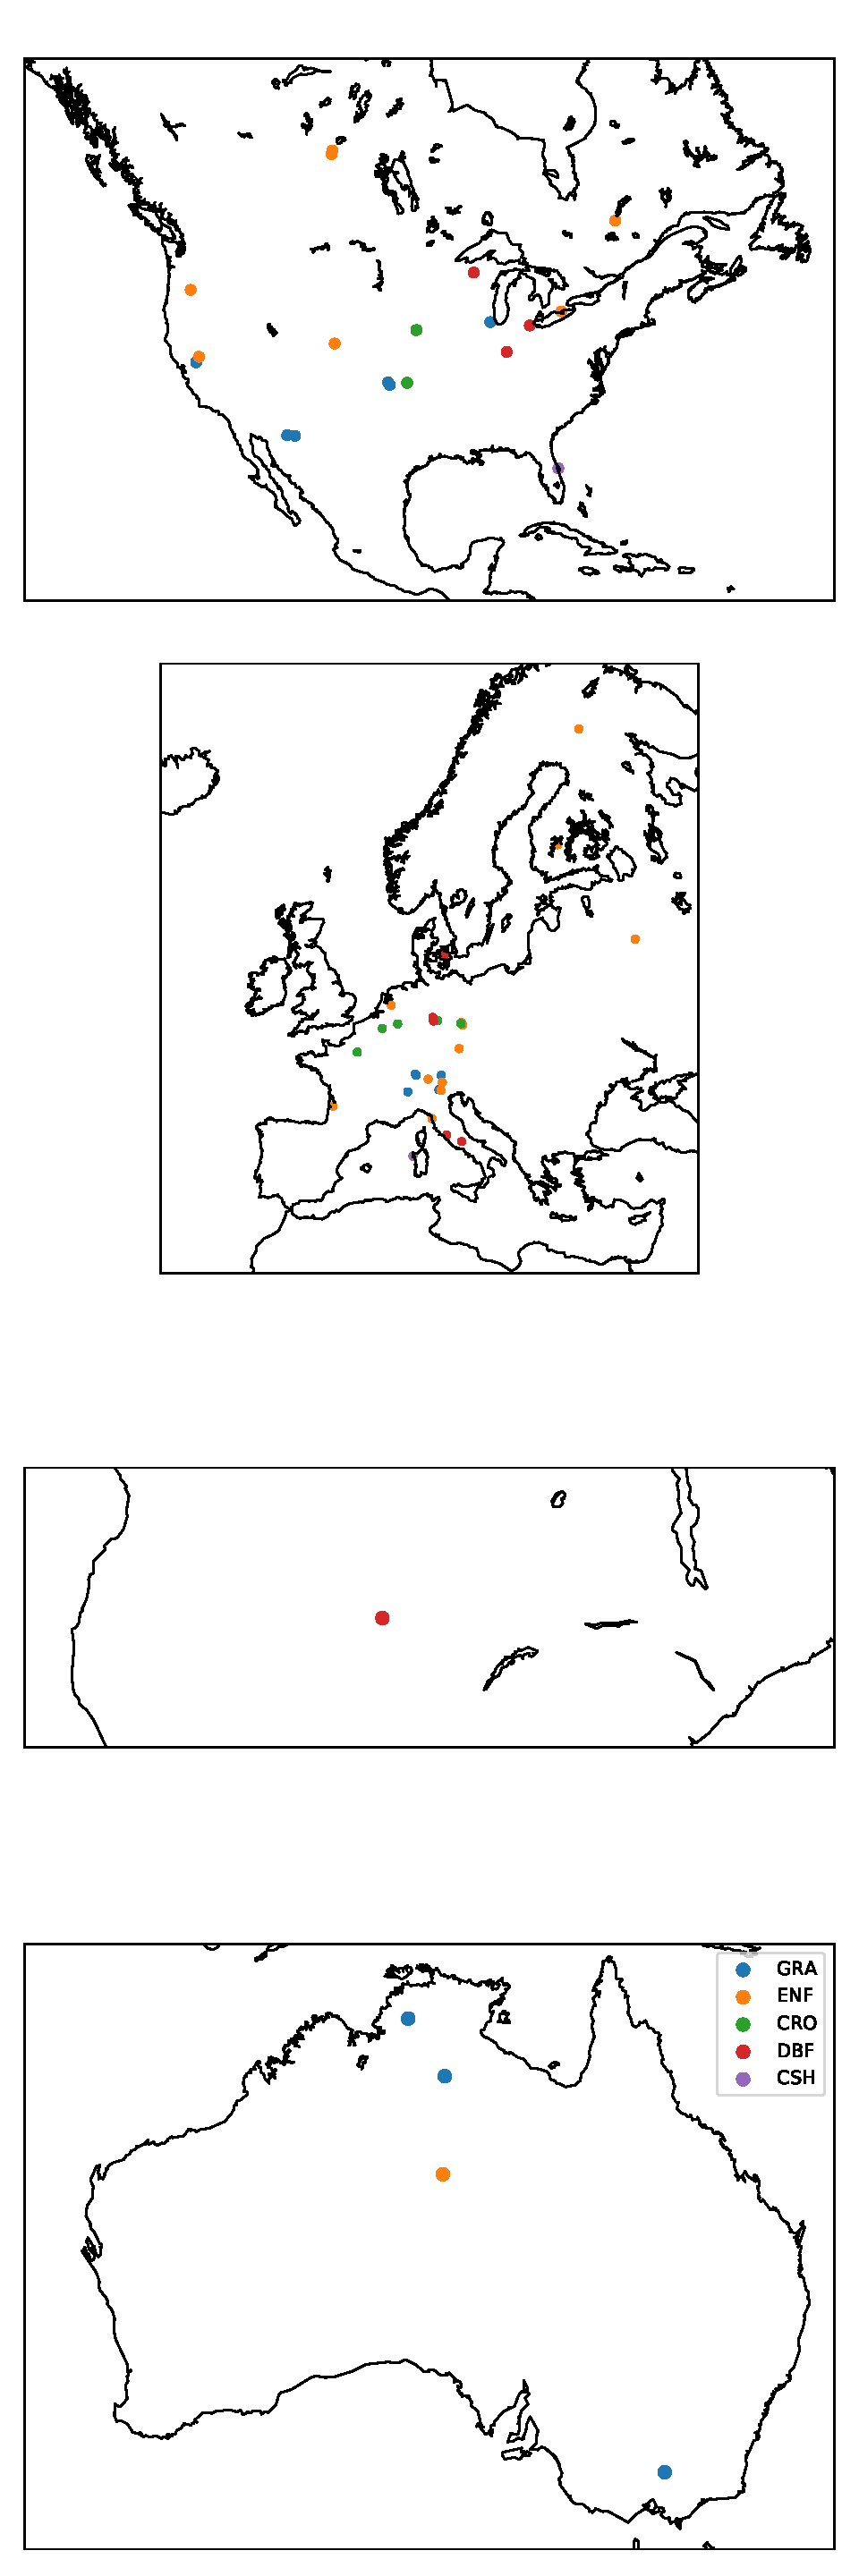
\includegraphics[width=20pc]{./fig01.pdf}
\caption{Plant functional type and location of sites used in analysis. ***\textbf{This is just  a placeholder for now, I am currently fixing it***}}
\label{map_fig}
 \end{figure}

\section{Results}
\label{results}

By construction, the variability in the $\sigma$ term (Equation \ref{sigma}) contains all model and observational uncertainties. For an observation that perfectly matches our model and constant uWUE assumption $\sigma$ will be one. Therefore, for our assumptions and framework to be reasonable $\sigma$ should be $O(1)$. Figure \ref{lai_fig} presents the histogram of calculated $\sigma$s with outliers removed (lowest and highest 5\% percent). All remaining $\sigma$ values are close to unity ($O(1)$) which provides confidence in model framework.

\begin{figure}[h]
\centering
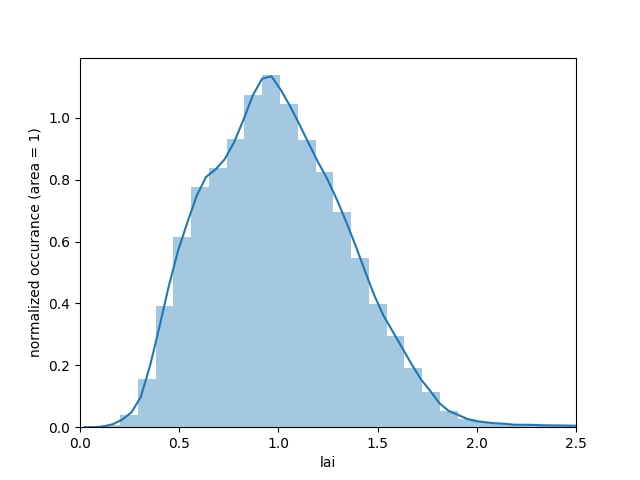
\includegraphics[width=20pc]{./fig02.png}
\caption{Histogram of $\sigma$ values calculated for each site and time according to Equation \ref{sigma}. The lowest and highest 5\% are removed as outliers, as well as any values below 0. The curve is normalized such that its area is 1. }
\label{lai_fig}
\end{figure}

An additional concern is that $\sigma$ may in fact be correlated with $VPD$, in which case the dependence would need to be accounted for when taking the derivative. Figure \ref{lai_vpd_fig} plots the joint distribution of $\sigma$ and VPD, and shows that $\sigma$ is very weakly a function of VPD. Given this weak dependence, we argue that Equation \ref{d_et} is a valid approximation for ET response to $VPD$.

\begin{figure}[h]
\centering
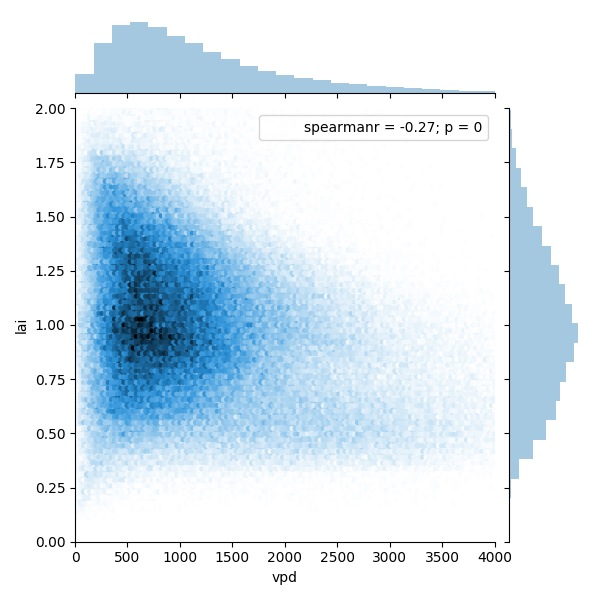
\includegraphics[width=20pc]{./fig03.png}
\caption{The joint distribution of $VPD$ and $\sigma$. $\sigma$ has only a weak dependence on $VPD$. \textbf{***note I am redoing/cleaning up this plot, ``lai'' should read sigma***}}
\label{lai_vpd_fig}
\end{figure}

Before calculating the sensitivity of ET to VPD, we will consider the functional form of Equation \ref{d_et}. There are two main terms: a ``scaling'' term, which modifies the magnitude but not the sign of the derivative $\partial ET/\partial VPD$:

\begin{equation}
  \frac{g_a \; P}{T(\Delta + \gamma)},
\end{equation}

and a ``sign'' term, which determines whether the derivative is positive i.e. atmospheric demand driven or negative i.e. physiologically controlled:

\begin{equation}
  \label{sign}
  \frac{c_p}{R_{air}} - \frac{\gamma c_s }{1.6 \; R\; \text{ uWUE }} \left( \frac{2 g_1 + \sqrt{VPD}}{2 (g_1 + \sqrt{VPD})^2}\right).
\end{equation}
All variables are positive, so the relative magnitude between the first term and the second term in Equation \ref{sign} will determine whether ET increases or decreases with increasing VPD. If the second term is larger magnitude then plant response dominates, while if the first term is larger then atmospheric demand dominates. The sign will determine whether ET is increasing or decreasing and we thus evaluate its functional form first. 

\subsection{Functional Form of the Sign Term}
\label{sign_func}
First, we explore the variables within the sign term to gain better intuition on the driver of either the increase or reduction of ET with VPD. $c_s$ and $\gamma$ are relatively constant to a good approximation so that the variability is dominated by $\sigma$ and $VPD$. $uWUE$ could vary with soil moisture but has been shown to be relatively constant except in very dry soil conditions \citep{Zhou_2016, Lin_2015}. We thus further assume that the soil is not too dry so that $uWUE$ can be approximated as a constant. This then means that the sign term only depends on VPD for a given PFT and is approximately just a function of $VPD$. We can further determine a critical threshold separating an increase from decrease in ET, such that $VPD_{crit}$ where $\frac{\partial \; ET}{\partial \; VPD} = 0$:

\begin{linenomath*}
  \begin{equation}
VPD_{crit} = \frac{R_{air}}{4 c_p} \left( \frac{\gamma c_s}{1.6\; R \; \overline{\sigma} uWUE} + \sqrt{\frac{\gamma c_s}{1.6\; R \; \overline{\sigma} uWUE}\left( \frac{\gamma c_s}{1.6\; R \; \overline{\sigma} uWUE} + 8 g_1 \frac{c_p}{R_{air}}\right)} - 4 g_1 \frac{c_p}{R_{air}} \right)
\label{vpd_min_et}
  \end{equation}
\end{linenomath*}

Values of $VPD_{crit}$ as a function of PFT are shown in Table \ref{vpd_crit}. For any values of $VPD$ less than $VPD_{crit}$, $\frac{\partial \; ET}{\partial \; VPD}$ will be negative, and for values of $VPD$ greater than $VPD_{crit}$, $\frac{\partial \; ET}{\partial \; VPD}$ will be positive. In other words, ecosystems can regulate and mitigate evaporative losses up to a VPD limit, above which atmospheric demand is just too high to be entirely compensated by stomatal regulation. We note however that even though ET increases again above the critical threshold, $VPD_{crit}$, ET is still much lower that potential evaporation as stomata are stills strongly regulating vapor fluxes. Even in the absence of soil pore evaporation, stomata do not shut down entirely at very high VPD and ET does not go to zero, because stomata are still slightly open to perform some photosynthesis \citep{Ball_1987, Leuning_1990, Medlyn_2011}. In addition, upward xylem transport is necessary to maintain phloem transport and thus carbon allocation (MENCUCCINI) \explain{Not sure citation  - Comparative criteria for models of the vasuclar transport systems of tall trees}.

\begin{table}
  \label{vpd_crit}
\caption{Values of $VPD_{crit}$, where $\frac{\partial \; ET}{\partial \; VPD} = 0$, evaluated at PFT average values for $R_{air}$, $\sigma$, $\gamma$, and $c_s$. For reference, these values are also provided CITE TABLE. For values of $VPD$ less than $VPD_{crit}$, $\frac{\partial \; ET}{\partial \; VPD}$ will be negative, and for values of $VPD$ greater than $VPD_{crit}$, $\frac{\partial \; ET}{\partial \; VPD}$ will be positive. \textbf{**** this statistics are dated, need to update***}}
\centering
\begin{tabular}{l c c c c c c}
  \hline
  PFT & $R_{air}$ & $c_s$ (ppm) & $\gamma$ &  uWUE    & \textbf{$VPD_{crit}$ (Pa)} \\
  \hline
  CRO &  288.680920 & 372.567691& 65.351523& 2.602873&  \textbf{133.165438} \\
  CSH &   289.067152& 381.593622& 67.613172& 2.175278& \textbf{4439.564212} \\
  DBF &   288.624437& 377.449849& 63.421812& 2.746393&  \textbf{888.773243} \\
  ENF &  288.183849& 377.676463& 61.559242& 4.015362&  \textbf{978.084845} \\
  GRA &  288.425651& 377.264645& 61.598768& 2.281074& \textbf{1141.630778} \\
\hline
\multicolumn{2}{l}{$^{a}$Footnote text here.}
\end{tabular}
\end{table}

Differences in $uWUE$ and $g_1$ between PFTs alter the functional form of the sign term.  Larger $uWUE$ and $g_1$ will shift the sign term towards overall positive values. $g_1$ additionally plays a primary role in determining dependnece on VPD: the smaller $g_1$, the greater the $VPD$ dependence for the PFT (Figure \ref{term3}).

Based on Figure \ref{term3} and Table \ref{vpd_crit}, CROs are the least water conservative and have the most positive constant offset, while CSH are the most water conservative and have the most negative constant offset in the sign term.  ENF ($g_1 = 74.31$) has by far the largest VPD dependence of response, while CRO ($g_1 = 183.1$) has the smallest VPD dependence. ENF are less willing to trade water for new growth, so the regulate water much more strongly depending on the dryness environment (VPD). CRO on the otherhand are more willing to trade water for new growth, so they regulate water relatively similiarly irregardless of the environment.
 
A primary takeaway from Figure \ref{term3}a is that according to our theory for all PFTs except for crops there is frequent occurrence of a negative (plant dominating) ET response to increases in VPD. This thus means that plants are able in most atmospheric conditions to redue ET in response to increased VPD and thus to reduce water losses. To better illustrate this, the ranges of observed environmental VPDs at the FLUXNET sites are plotted parallel to the x-axis. For CSH, VPD is always less than VPD$_{crit}$ so that the plant response dominates and empathizes the water conservative strategy of those plants. For CRO on the other, VPD is almost always higher than VPD$_{crit}$, emphasizing that those plants are water intensive and were actually engineered for photosynthesis rather than water saving. For forests and grass, whether plant response or atmospheric demand dominates is more dependent on the environment, with about half of of observed VPD less than VPD$_{crit}$, i.e. in conditions where plant response dominates. It is also important to note that even when atmospheric demand dominates, the response is still far smaller than it would be for potential evaporation i.e. atmospheric demand only, emphasizing that there is still a strong regulation of evaporative flux by stomata and though the plant xylem. The sign term in this case would just be a constant ($\frac{c_p}{R_{air}} \approx 3.5$), which is far larger than any part of the curves for any PFT. This highlights the deficiencies of PET's ability to capture land response to changes in atmospheric dryness (VPD). Plants are always regulating water exchange from the land surface, even when they reach the limits of they ability to do so. Therefore, the actual land surface reponse to a change in VPD will always me more negative than if the plants are not included in the physics (PET). However, we have assumed $\sigma$ (uncertainty) equal to one. We still need to test if inclusion of uncertainty could change our conclusions.
\begin{figure}[h]
\centering
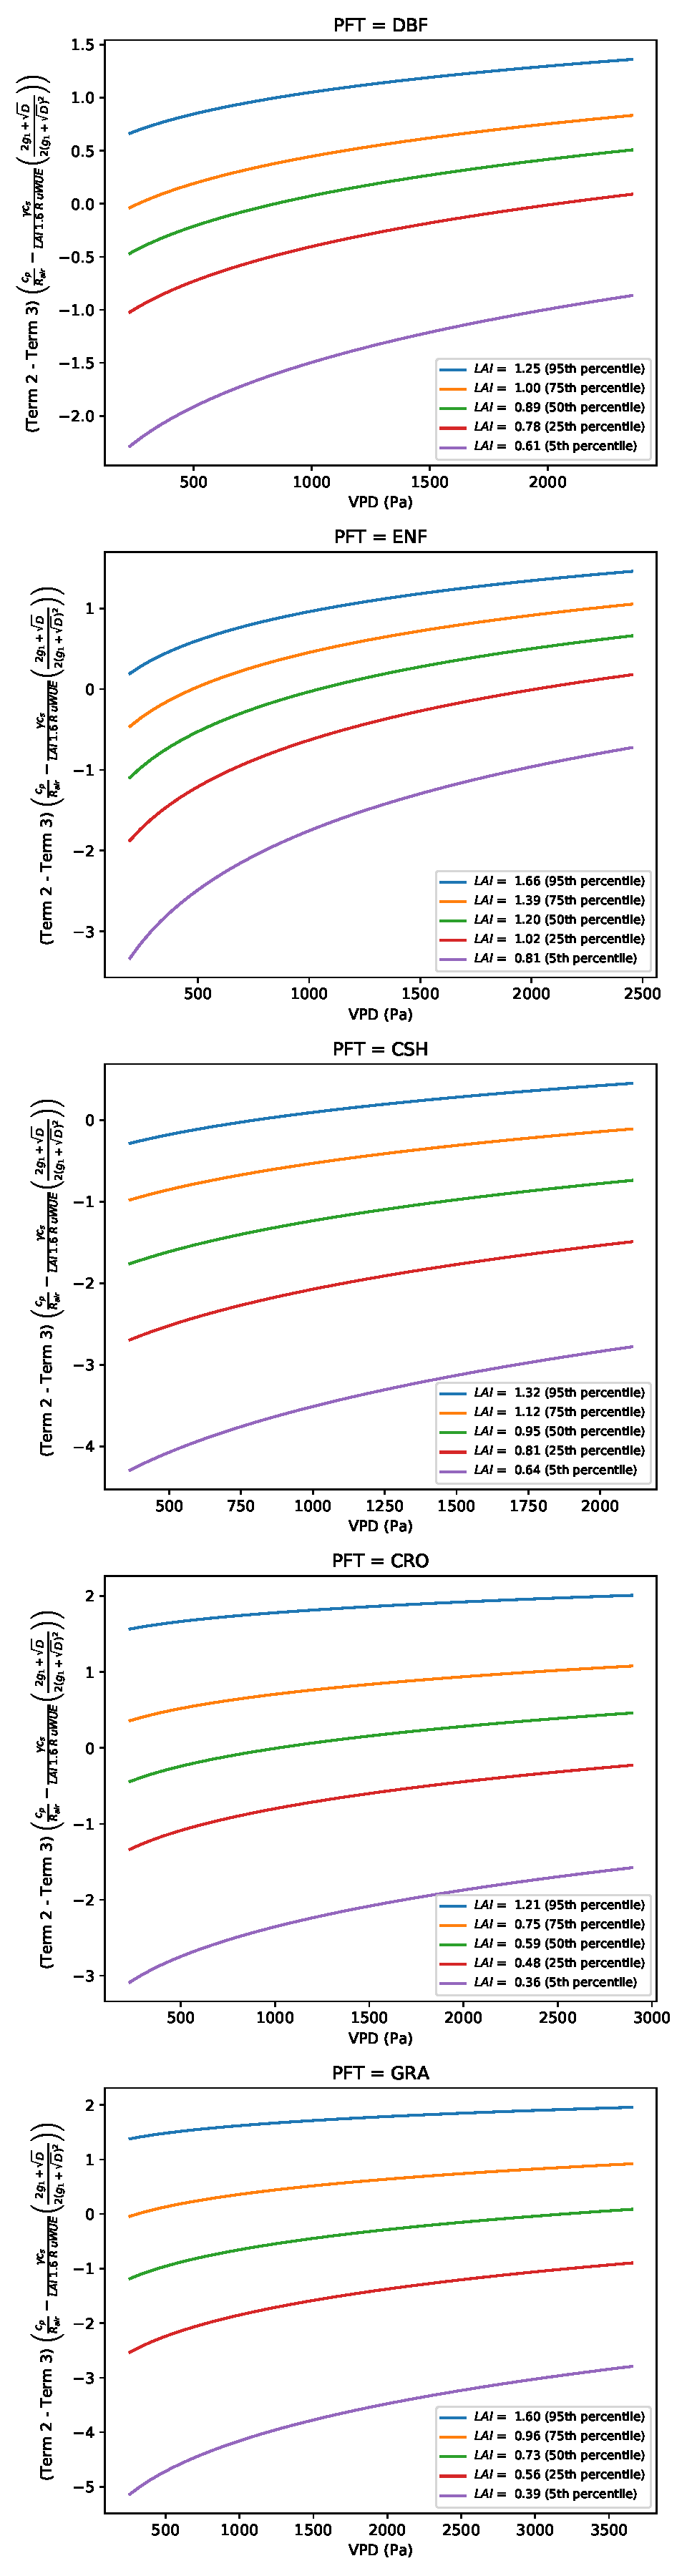
\includegraphics[width=20pc]{./fig05.pdf}
\caption{Sources of variability for the sign term. Top: sign term as a function of VPD, with $\sigma$ held fixed at 1. The observed range of VPD for each PFT is also shown below the x-axis. Line extent corresponds to 5th and 95th percentiles, while stars denote the location of the 25th, 50th, and 75th percentiles.

Bottom: The location of the minima of ET, as a function of VPD and $\sigma$. Lines and stars denote the distribution of VPD and $\sigma$ next to each axis, following the same percentiles as above. \textbf{***need to replot with correct sigma (normalized to 1), also correct uWUE label in first plot***}}
\label{term3}
\end{figure}

Figure \ref{term3}b shows the location of VPD$_{crit}$, as a function of $\sigma$ (uncertainty) and $VPD$. For any $\sigma$ or VPD less (more) than these curves, the sign term will be negative (positive). It is clear that the portion of VPD observations below/above these curves will be a strong function of $\sigma$. This motivates a thorough examination of how inclusion of uncertainty ($\sigma$) might change the form of the sign term, and in particular the location of VPD$_{crit}$ for each of our plant types. In Secion \ref{testing} we examine if and how uncertainty changes the analysis presented in this section, for each PFT.

\subsection{Functional Form of the Scaling Term}

While the above discussion of the sign of $\frac{\partial \; ET}{\partial \; VPD}$ is important to answer our research question, the magnitude of $\frac{\partial \; ET}{\partial \; VPD}$ will also the relative magnitude of the change $\frac{\partial \; ET}{\partial \; VPD}$ and the importance of $VPD$ variability for overall $ET$ variability. So we now more closely examine the scaling term: $\frac{P}{T} \propto \rho$. Air density $\rho$ scaling term varies little relative to aerodynamic conductance and $\Delta$. The psychrometric constant $\gamma$ is also relatively constant, so the scaling term should be primarily a function of aerodynamic conductance and temperature, through the slope of the Clauisu-Clapeyron relationship $\Delta$. This is as expected, given that the aerodynamic conductance represents the efficiency fo the transfer of surface anomalies to the atmosphere. As aerodynamic conductace  increases, any plant response will be communicated more strongly to the atmosphere (and vice-versa).

$\Delta$'s presence in the scaling term also matches physical intuition. Evaporative cooling will dampen the ability of the atmosphere to take more moisture, because $e_{s}$ decreases with decreasing temperature. The decrease in $e_{s}$ is proportional to $\Delta$ ($\delta e_{s} = \Delta \delta T$). So as $\Delta$ increases, you will get a larger damping of ET due to evaporative cooling.  The functional from of $\Delta$ will be the same across PFT, but the temperature range may vary slightly. In contrast, aerodynamic conductance will vary strongly with PFT due to the importance of surface roughness. So most of the differences in scaling between PFT should be in the aerodynamic conductance term. One interesting side note is that the coefficient of variability for both aerodynamic conductance and the scaling term is relatively constant across PFT, suggesting that the influence of aerodynamic conductance on the relative (to the PFT mean) variability of the scaling term is approximately similar across PFT.

Figure \ref{scale_vary}A shows the scaling term normalized by mean aerodynamic conductance (calculated for each plant functional type), and confirms that much of the relative variability of the scaling term is caused by aerodynamic conductance variability. Generally, temperature (via $\Delta$) causes less relative variability. However, the impact of $T$ on the relative variability increases with increasing aerodynamic conductance. 

While the relative variability of scaling term is similar across PFT, the absolute value of scaling term varies strongly across PFT. Figure \ref{scale_vary}B shows scaling term evaluated at the mean aerodynamic conductance for each PFT, and at the range of observed temperatures for each PFT. As expected, for the tree PFTs (DBF, ENF) the scaling term is much larger and the temperature dependence is much stronger. Systematic differences in observed temperatures also cause differences in the average magnitude of scaling term. For example, ENF experiences on average colder temperatures and is thus more likely to have a larger scaling term. Additionally, because the variability of aerodynamic conductance increases proportionally to the mean, the spread of the scaling term due to aerodynamic conductance variability will be larger for the tree PFTs, although this is not shown for simplicity. To summarize Figure \ref{scale_vary}: the variability of the scaling term within each PFT will look like Figure \ref{scale_vary}A for each PFT, but the scale of the y-axis will increase or decrease according to mean aerodynamic conductance observed in Figure \ref{scale_vary}B.
 
\begin{figure}[h]
\centering
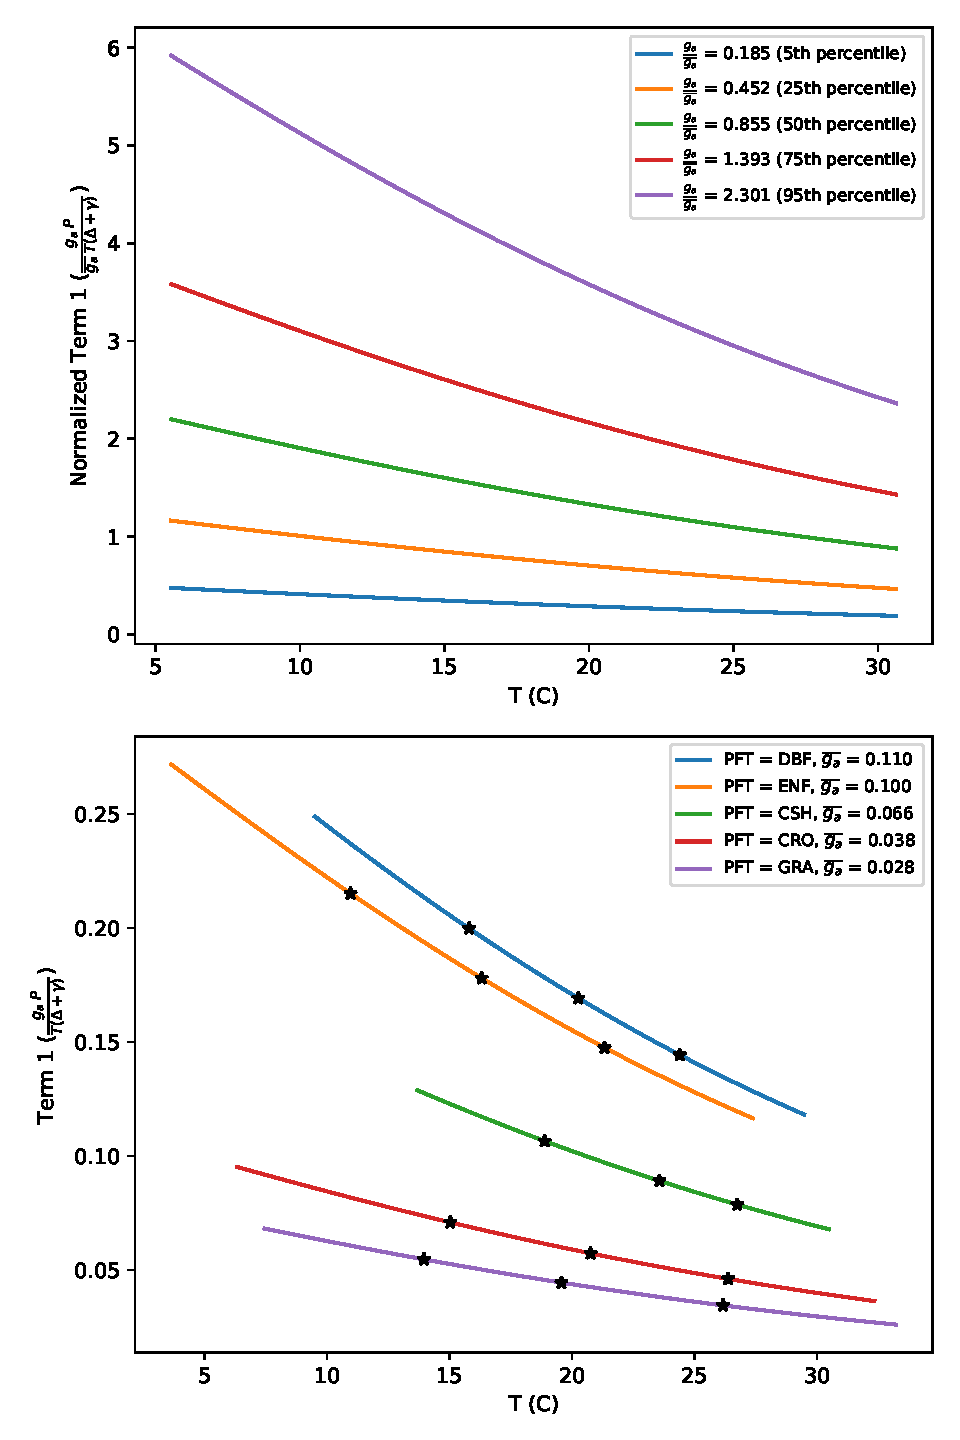
\includegraphics[width=20pc]{./fig04.pdf}
\caption{Primary sources of variability for scaling term. A) Variability within each PFT: scaling term normalized by mean $g_a$ for each PFT. B) Variability between each PFT: scaling term evaluated at mean $g_a$ for each PFT. Temperature range is 5-95th percentile for each PFT. Additionally, stars denote the location of the 25th, 50th, and 75th percentiles.}
\label{scale_vary}
\end{figure}

%%%%% replace below with idea:
\subsection{Bulk statistics of $\frac{\partial \; ET}{\partial \; VPD}$}

Table 3 confirms our expectations for PFT behavior of $\frac{\partial \; ET}{\partial \; VPD}$. For all PFTs except for CRO, average $\frac{\partial \; ET}{\partial \; VPD}$ is less than zero. However, $\frac{\partial \; ET}{\partial \; VPD}$ evaluated at the average of all variables (e.g. $\sigma$, $T$, $c_s$, $VPD$) is only negative for CSH and GRA. And, DBF in addition to CRO experiences $\frac{\partial \; ET}{\partial \; VPD}$ < 0 less than half the time. These observations highlight the effect of the nonlinear function in Figure \ref{term3}: $\frac{\partial \; ET}{\partial \; VPD}$ has a much steeper slope when the function is negative, and is thus more likely to be large magnitude.

The units of $\frac{\partial \; ET}{\partial \; VPD}$ make it difficult to interpret if $VPD$ is even a meaningful contributor to ET's variability. To better understand $VPD$'s contribution, we multiply $\frac{\partial \; ET}{\partial \; VPD}\left(\overline{env}\right)$ with $VPD$'s standard deviation to define a (linearized) relative change in ET for variations in $VPD$ . $VPD$'s contribution to ET's variability ranges between 30 - 40 W m$^{-2}$ for all PFTs except for CSH, which is about 100 W m$^{-2}$. Another meaningful comparison is to $\frac{\partial \; ET}{\partial \; R} \cdot std(R)$, as net radiation is generally the driver of ET (cite joe berry here)\explain{Find citation?}. For all PFTs except for CSH $VPD$ contributes between 30 - 40 \% of $R$'s contribution to variability. For CSH the portion is much larger, about 88 \%. $VPD$'s variability is certainly a non-negligible contributor to $ET$'s variability.

Theoretical derivation has so far illuminated the dependence of $\frac{\partial \; ET}{\partial \; VPD}$ and how it varies across PFT. Large mean $uWUE$ shifts CRO and DBF towards a tendancy to increase ET with VPD (positive $\frac{\partial \; ET}{\partial \; VPD}$), but a lower slope parameter ($g_1$) for DBF allows for decreaes in ET with VPD, at low environmental VPD. \explain{physically state how slope parameter is trade for water at leaf level, but uWUE is trade-ff between GPP and VPD at ecosystem-level}.  ENF's very low slope parameter ($g_1$), which is even lower than for DBF, increases the dependence of ET response  ($\frac{\partial \; ET}{\partial \; VPD}$) on $VPD$, and makes the function strongly nonlinear. This has the effect of making mean ET response ($\overline{\frac{\partial \; ET}{\partial \; VPD}}$)  more negative for a given frequency of occurence of negative ET response ($\frac{\partial \; ET}{\partial \; VPD} < 0$), than for other PFT. GRA shows the opposite behavior; a relatively high slope parameter ($g_1$)  makes the function more linear, causing a more positive mean ET reponse ($\overline{\frac{\partial \; ET}{\partial \; VPD}}$) for a given given frequence of negative ET reponse  ($\frac{\partial \; ET}{\partial \; VPD} < 0$). Finally, CSH's very low $uWUE$ dominates the slope parameter's effects, causing ET to almost always decrees with increasing atmospheric dryness (VPD), even with uncertainty included. Variability in $VPD$ accounts for the largest amount of $ET$ variability for CSH. For the other PFTs, $VPD$ contributes less to $ET$ variability, but still represents about 30-40 \% of $R$'s contributions to ET variability. \explain{think pierre is correct, could probably scrap this anecdote: WHAT IS THE SORUCE OF VARIBILITY OF THE REST OF ET I DON"T KNOW IF THAT IS RELEVANT FOR THE PRESENT PAPER.}

\begin{table}
\caption{Statistics of $\frac{\partial \; ET}{\partial \; VPD}$ as a function of PFT. \textbf{***dated, need to update these statistics***}}
\centering
\begin{tabular}{l c c c c c}
  \hline
PFT & $\overline{\frac{\partial \; ET}{\partial \; VPD}}$ & $\frac{\partial \; ET}{\partial \; VPD}\left(\overline{env}\right)$ & $\frac{\partial \; ET}{\partial \; VPD}\left(\overline{env}\right)*\text{std}(VPD)$ & $\frac{\frac{\partial \; ET}{\partial \; VPD}\left(\overline{env}\right)*\text{std}(VPD)}{ \frac{\partial \; ET}{\partial \; R}\left(\overline{env}\right)*\text{std}(R)}$ & fraction $\frac{\partial \; ET}{\partial \; VPD} < 0.$ \\
  \hline
CRO & 0.000853 & 0.026241 & 37.05 & 0.41 & 0.473311\\
CSH & -0.108234 & -0.091526 & 101.72 & 0.88 & 0.931660\\
DBF & -0.012727 & 0.013794 & 39.47 & 0.33 & 0.461674\\
ENF & -0.034087 & 0.000706 & 33.22 & 0.30 & 0.534425\\
GRA & -0.019637 & -0.000921 & 33.60 & 0.35 & 0.631735\\
\hline
  
\end{tabular}
\end{table}


\subsection{Validation of theory at eddy-covariance sites}
\label{testing}
So far we have developed a theory for $\frac{\partial \; ET}{\partial \; VPD}$'s behavior as a function of VPD and PFTs. We now turn to an direct evaluation against observations taken from a wide range of eddy-covariance datasets (Section \ref{methods}).

Figure \ref{agu_fig} shows the distribution of of the sign term (when uncertainty is included), as compared to what the theory would predict. Our goal was to capture the leading order behavior of the ET dependence on VPD. Given the assumptions we have made, and the uncertainties of flux tower observations themselves, we expect a large amount of noise when reprdrocuing the derivatives of ET.

For DBF our theory is successful towards this goal: the theory matches the leading order behavior of the function when uncertainty is included, and the DBG figure looks as one would expect if one just added noise on top of our theory. The VPD dependence, given by the slope parameter ($g_1$), floows the median values of each box plot. Perhaps most importantly, the x-intercept, and thus VPD$_{crit}$, matches nearly exactly between the theory and the observations. Therefor the sign of the ET response to increases in VPD should be well matched, subject to the unavoidable constraints of noise, much of which may be from the observations themselves. The uncertainty is non negligable; there are bany observations in each box for which the the sign of observation is opposite the response predicted by the theory, but to leading order our theory matches the observations. 

While CSH has a much different functional form of the sign term than DBF, CSH observations also match our theory to leading order. Again, the VPD dependence mostly determined from the slope parameter ($g_1$) closely matches the medians in the observation bins. The VPD-independent, strongly negative response, which is determined by $uWUE$, is also captured. For CSH, there is extremely rare occurence of positive ET response with VPD, even with uncertainty, so the sign of the theory almost always matches the sign of the observations, even with all of the uncertainty.

The theory does not match as well for CRO as for DBF and CSH. At low VPD the VPD dependence (due to $g_1$) is similiar to the leading order behavior of the observations, but the entire curve is shifted towards postiive values, due to some error in $uWUE$. Most strikingly, the observations show a tendency to move back towards negative values at high VPD, which given the functional form of VPD dependnce, is behavior that is impossible fo the theory to capture. This divergence between the theory and the observations for CRO could have been expected. For practical reasons, our theory does not include important sources of variability (particularly between sites) for CRO. We do not account for seasonal changes in LAI, variability in crop height and surface roughness, differences in C3 vs C4 photosynthesis, or differences in irrigation practices between the sites and/or years. This deficiencies would explain the inability of our theory to match obsercations. For example, a superpositions of sites with C3 plants (low VPD) and C4 plants (high VPD) would explain observed shift back towards negative ET reponse at high VPD when all sites are binned together, as in Figure \ref{agu_fig}.   

The theory for GRA suffers from similiar limitations as for CRO. The differences between the theory and the observations are more pronounced for GRA, but are explainable using similiar logic as that used for CRO. GRA will also have differences between sites in C3 vs C4 photosythesis, and irrigation practices, as well as strong seasonal variability in crop height and LAI. For GRA, the observations show a very different VPD dependence of response than the theory, with a strong tendency back toewards a negative ET reponse at high VPD which our theory cannot account for. As with CRO, this could be explained by a superposition of sites with C3 vs C4 sites. Unfortunately, because detailed site-level data of C3 vs C4 plant type, as well as irrigation practes, was difficult to obtain, we could not bin GRO and GRA further by irrigation and photosyethesis stragtegy. However, we hypothesize that the theory would much more closel match obsercations with photosythesis and irrigation are accounted for. 

The comparison between the theory and obsercations for ENF is unique from the rest of the PFTs. The VPD dependence of the theory, determined by the slope paramter, is not well captured by observations. However, the theory closely captures the x-intercept and VPD$_{crit}$. So, the theory still captures when the ET reponse will be positive or negative, but is less accurate with the magnitude of the reponse. Therefor the theory is still useful for addressing when VPD drives or reduces ET. Also, it's with noting that we used published constants for $g_1$ \citep[from ][]{Lin_2015}, which determines the VPD dependence. We could have fit our own constants so that the theory would best match the observations, but our goal was to use a priori physical constants whenever possible.

While the above discussion shows that our theory has some limitations when applied to some sites, especially for crops and grasslands, another question could be, how would using PET, as many hydrometeorological studies and applications do, compare with our theory.  Again, as in Section \ref{sign_func}, the PET response to changes in VPD will be constant at about 3.5. In Figure \ref{agu_fig} the ET reponse to shifts in dryness is always far more negative than 3.5 for the observations, even with all uncertainty included. So the PET reponse to atmospheric dryness is outside the range of all observable responses. This casts doubt on PET's usefulness for capturing the leading order behavior of water budgeting at the land surface. However our theory (Equation \ref{et}) could be used with published $uWUE$ and $g1$ as an alternative to PET to estimating land response and moisture budgeting.

\subsubsection{Testing VPD$_{crit}$}
As stated in the above discussion of ENF, we are mostly interested in the critical threshold $VPD_{crit}$ for which the sign of  $\frac{\partial \; ET}{\partial \; VPD}$ is determined. When $VPD < VPD_{crit}$, $\frac{\partial \; ET}{\partial \; VPD}  < 0$ (plant response dominates), and when $VPD > VPD_{crit}$, $\frac{\partial \; ET}{\partial \; VPD} > 0$ (atmospheric demand dominates). Theoretically this $VPD_{crit}$ is only a function of PFT. We can look at how this value of $VPD_{crit}$ matches the data as different observed variables (including uncertainty) are allowed to vary.


Figure \ref{real} presents calculated $\frac{\partial \; ET}{\partial \; VPD}$ where, unless otherwise noted, all variables in Equation \ref{d_et} are allowed to vary, including uncertainty. Each column represents a different quantity related to $\frac{\partial \; ET}{\partial \; VPD}$, and each row is a different PFT. Vertical black lines denote where our theory says $VPD_{crit}$ should be. For any observations to the left of this line $\frac{\partial \; ET}{\partial \; VPD}$ should be negative (plant response dominates), and any observations the right of the line should be positive (atmospheric demand dominates). In addition to seeing how our theoretically-derived VPD threshold, $VPD_{crit}$, matches observations, these analysis are also useful for observing how the scaling term affects the magnitude of the derivative, if at all. 

The scatter figures generally confirm expectations from Figure \ref{agu_fig}. By comparing different columns of Figure \ref{real} we can evaluate the impact of $\sigma$ and $g_a$ on the variability of $\frac{\partial \; ET}{\partial \; VPD}$. $g_a$'s scaling (included in columns 1 and 3) alters the magnitude considerably, particularly between PFTs. $\sigma$ variability (included in columns 1 and 2) adds a lot of additional noise to the signal of $\frac{\partial \; ET}{\partial \; VPD}$, as observed in Figure \ref{agu_fig}. However, the general story with the noise appears to match the cleaner signal when $\sigma$ is help constant and $VPD_{crit}$ is clearly visible. The exceptions are, as discussed above, for GRA and CRO, where the full complexity plots (Columns 1 and 2) do not match well with $\sigma$ held fixed (Columns 3 and 4).

While $g_a$ has a large impact on the magnitude of the scaling, temperature, through the derisive of the Clausius-Clapeyron, $\Delta$, term, does not appear to have as much of an impact in the complete estimation of $\frac{\partial \; ET}{\partial \; VPD}$. Therefore it appears that the absolute magnitude of the derivative can be mostly attributed to the sign term, and its direct scaling by aerodynamic conductance. Intuitively this is reasonable; aerodynamic conductance will control how dominant balances at the land surface are communicated to the boundary layer. While $\Delta$ controls the efficiency of latent fluxes in carrying heat away from the surface, it appears this is a second order term, relative to $g_a$, for scaling $\frac{\partial \; ET}{\partial \; VPD}$. 

In general Figures \ref{real} and \ref{agu_fig} match our expectations, even with the large sensitivity to $\sigma$ seen in Figure \ref{term3}. Our $\sigma$-based method of uncertainty propagation blurs the idealized expectations the most for GRA and CRO. We therefore have the most confidence in our conclusion based on Equation \ref{d_et} for PFTs CSH, DBF, and ENF, as the sign of the derivative with uncertainty included matches (to leading order) the story when $\sigma$ is held fixed.

\begin{figure}[h]
\centering
\includegraphics[width=\textwidth]{./agu_fig.pdf}
\caption{Comparison of the sign term with model uncertainty included (box plots) to the sign term as calculated with simplifying assumptions (blue line).}
\label{agu_fig}
\end{figure}


\begin{figure}[h]
\centering
\centerline{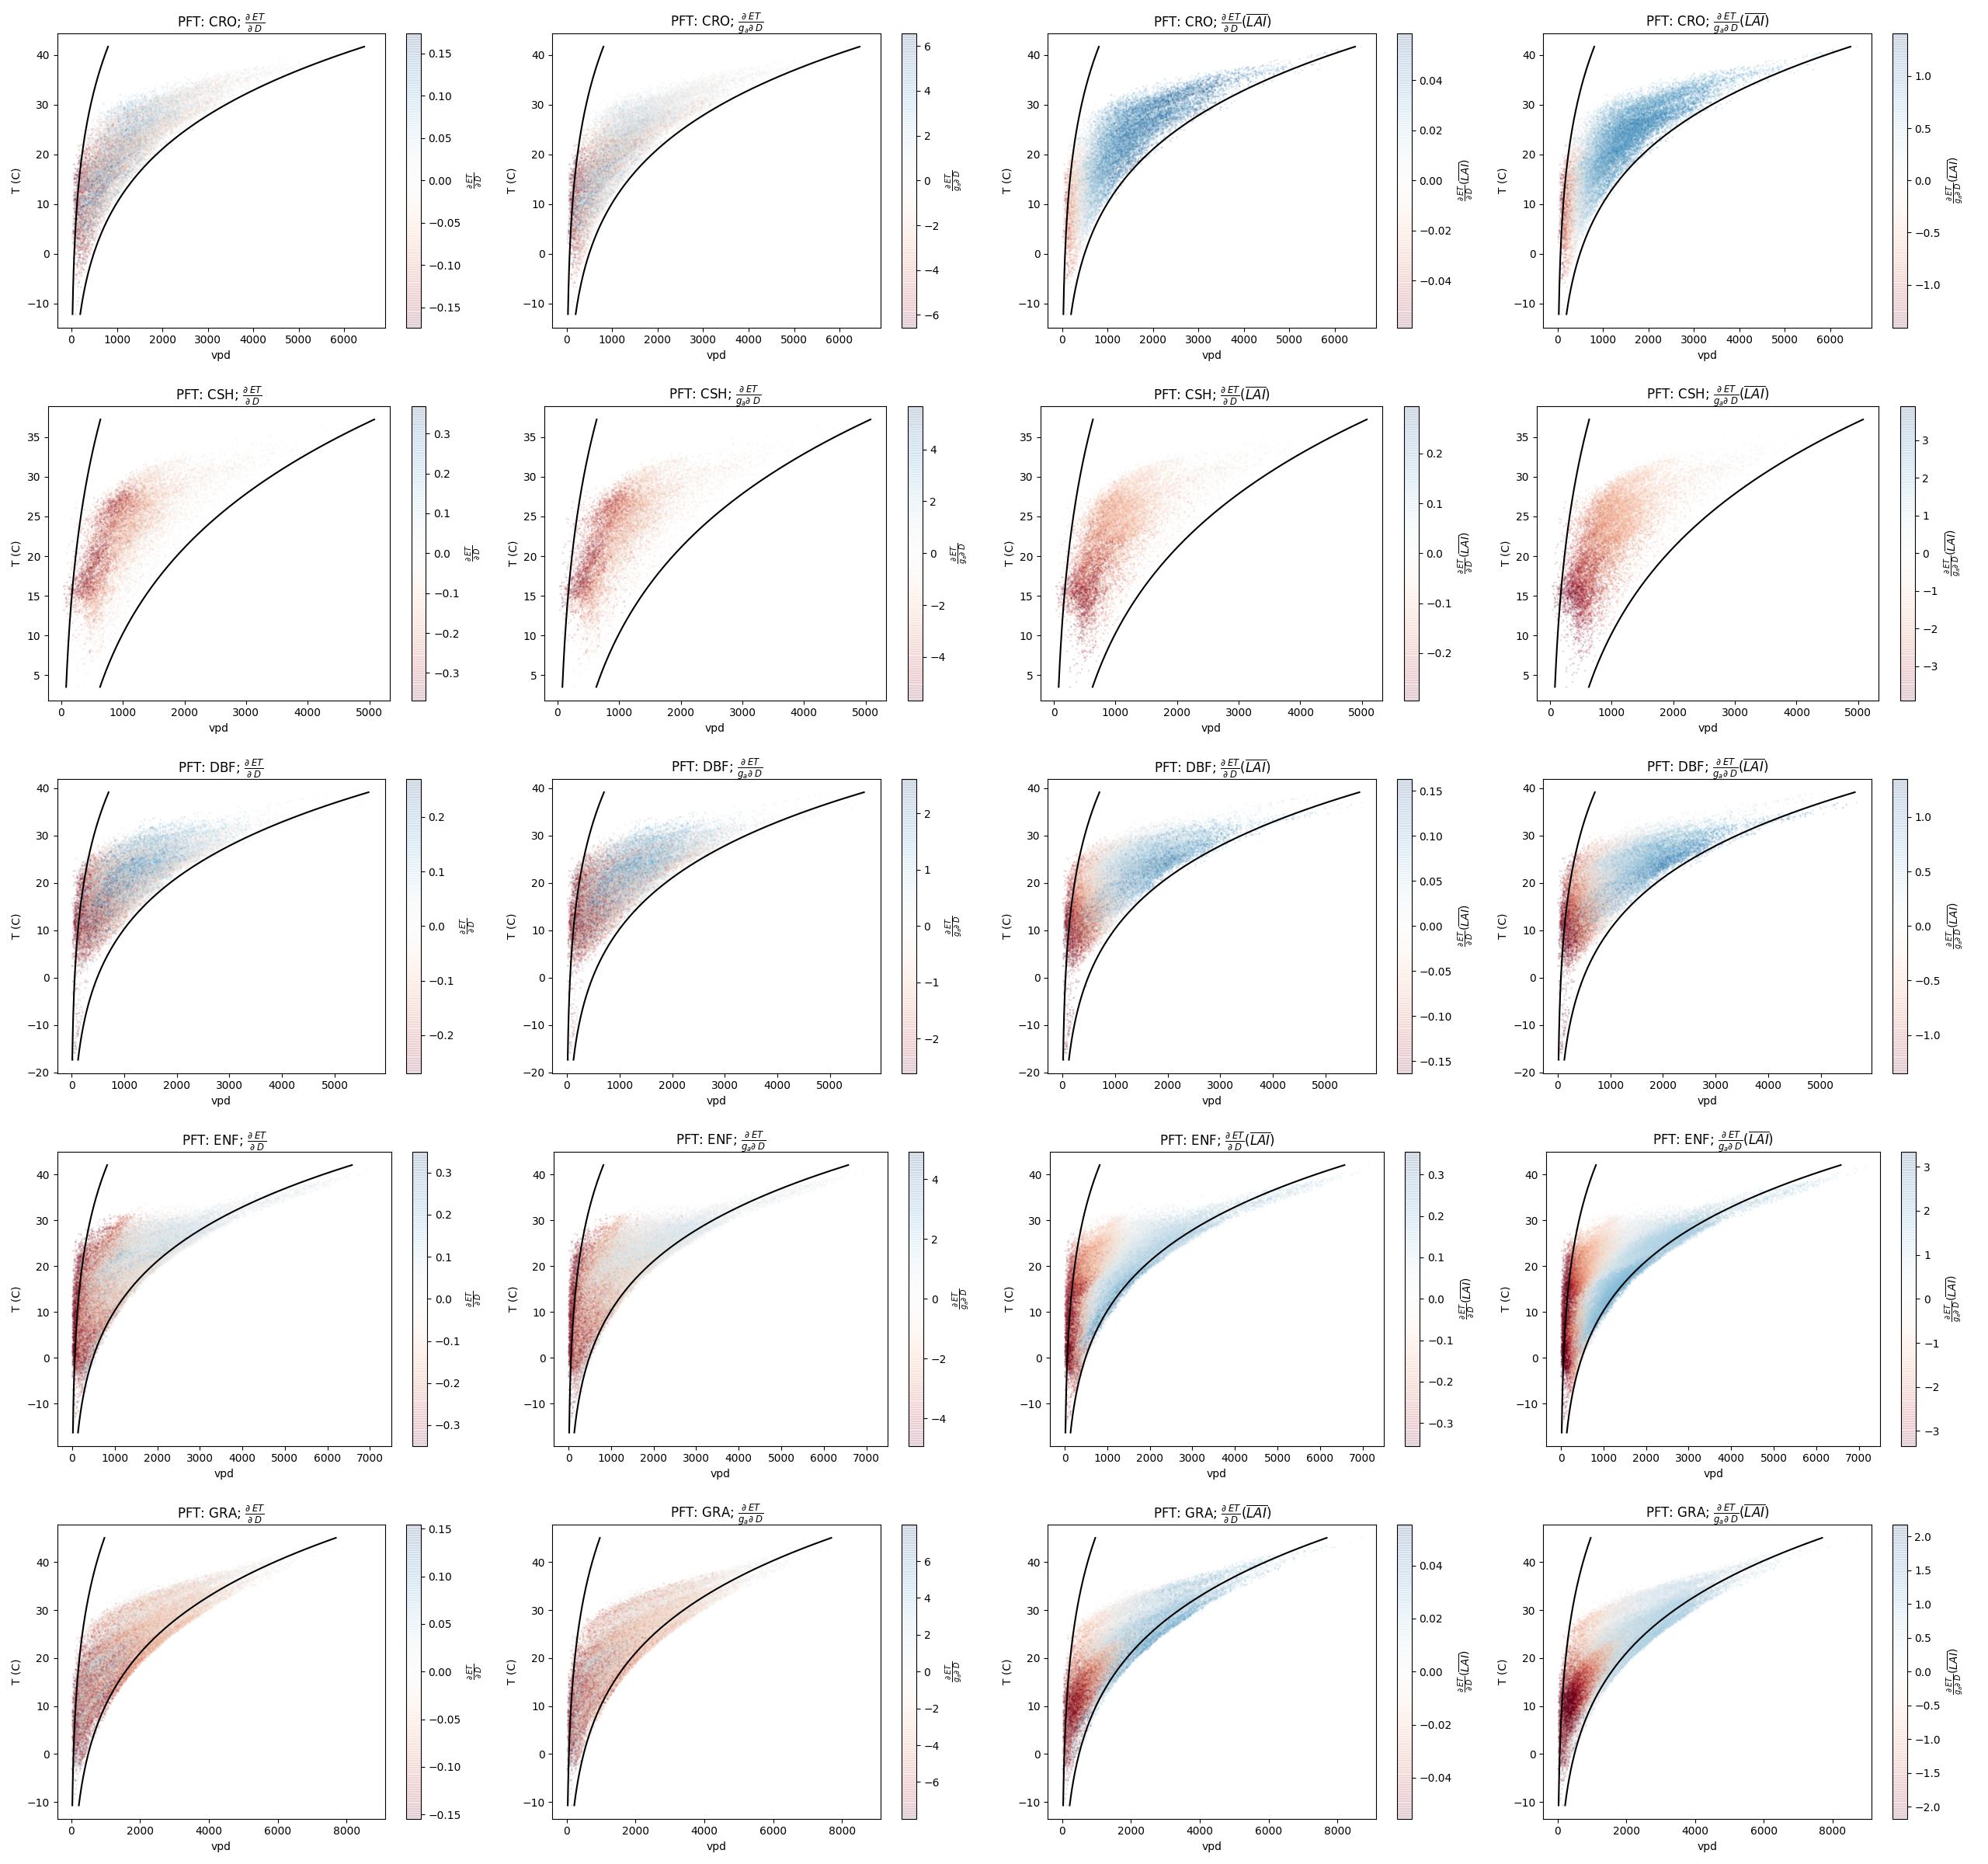
\includegraphics[width=1.4\textwidth]{./fig06.png}}
\caption{Scatter plots of $\frac{\partial \; ET}{\partial \; VPD}$. Each row is a different PFT, and each column is a different quantity related to $\frac{\partial \; ET}{\partial \; VPD}$, as labeled: Column 1: $\frac{\partial \; ET}{\partial \; VPD}$; Column 2: $\frac{\partial \; ET}{\partial \; VPD}$ normalized by $g_a$; Column 3: $\frac{\partial \; ET}{\partial \; VPD}$ with $\sigma$ held fixed at 1; and Column 4: $\frac{\partial \; ET}{\partial \; VPD}$ normalized by $g_a$ and with $\sigma$ held fixed. Please note differences in the colorbar scale.}
\label{real}
\end{figure}

% \begin{figure}[h]
% \centering
% 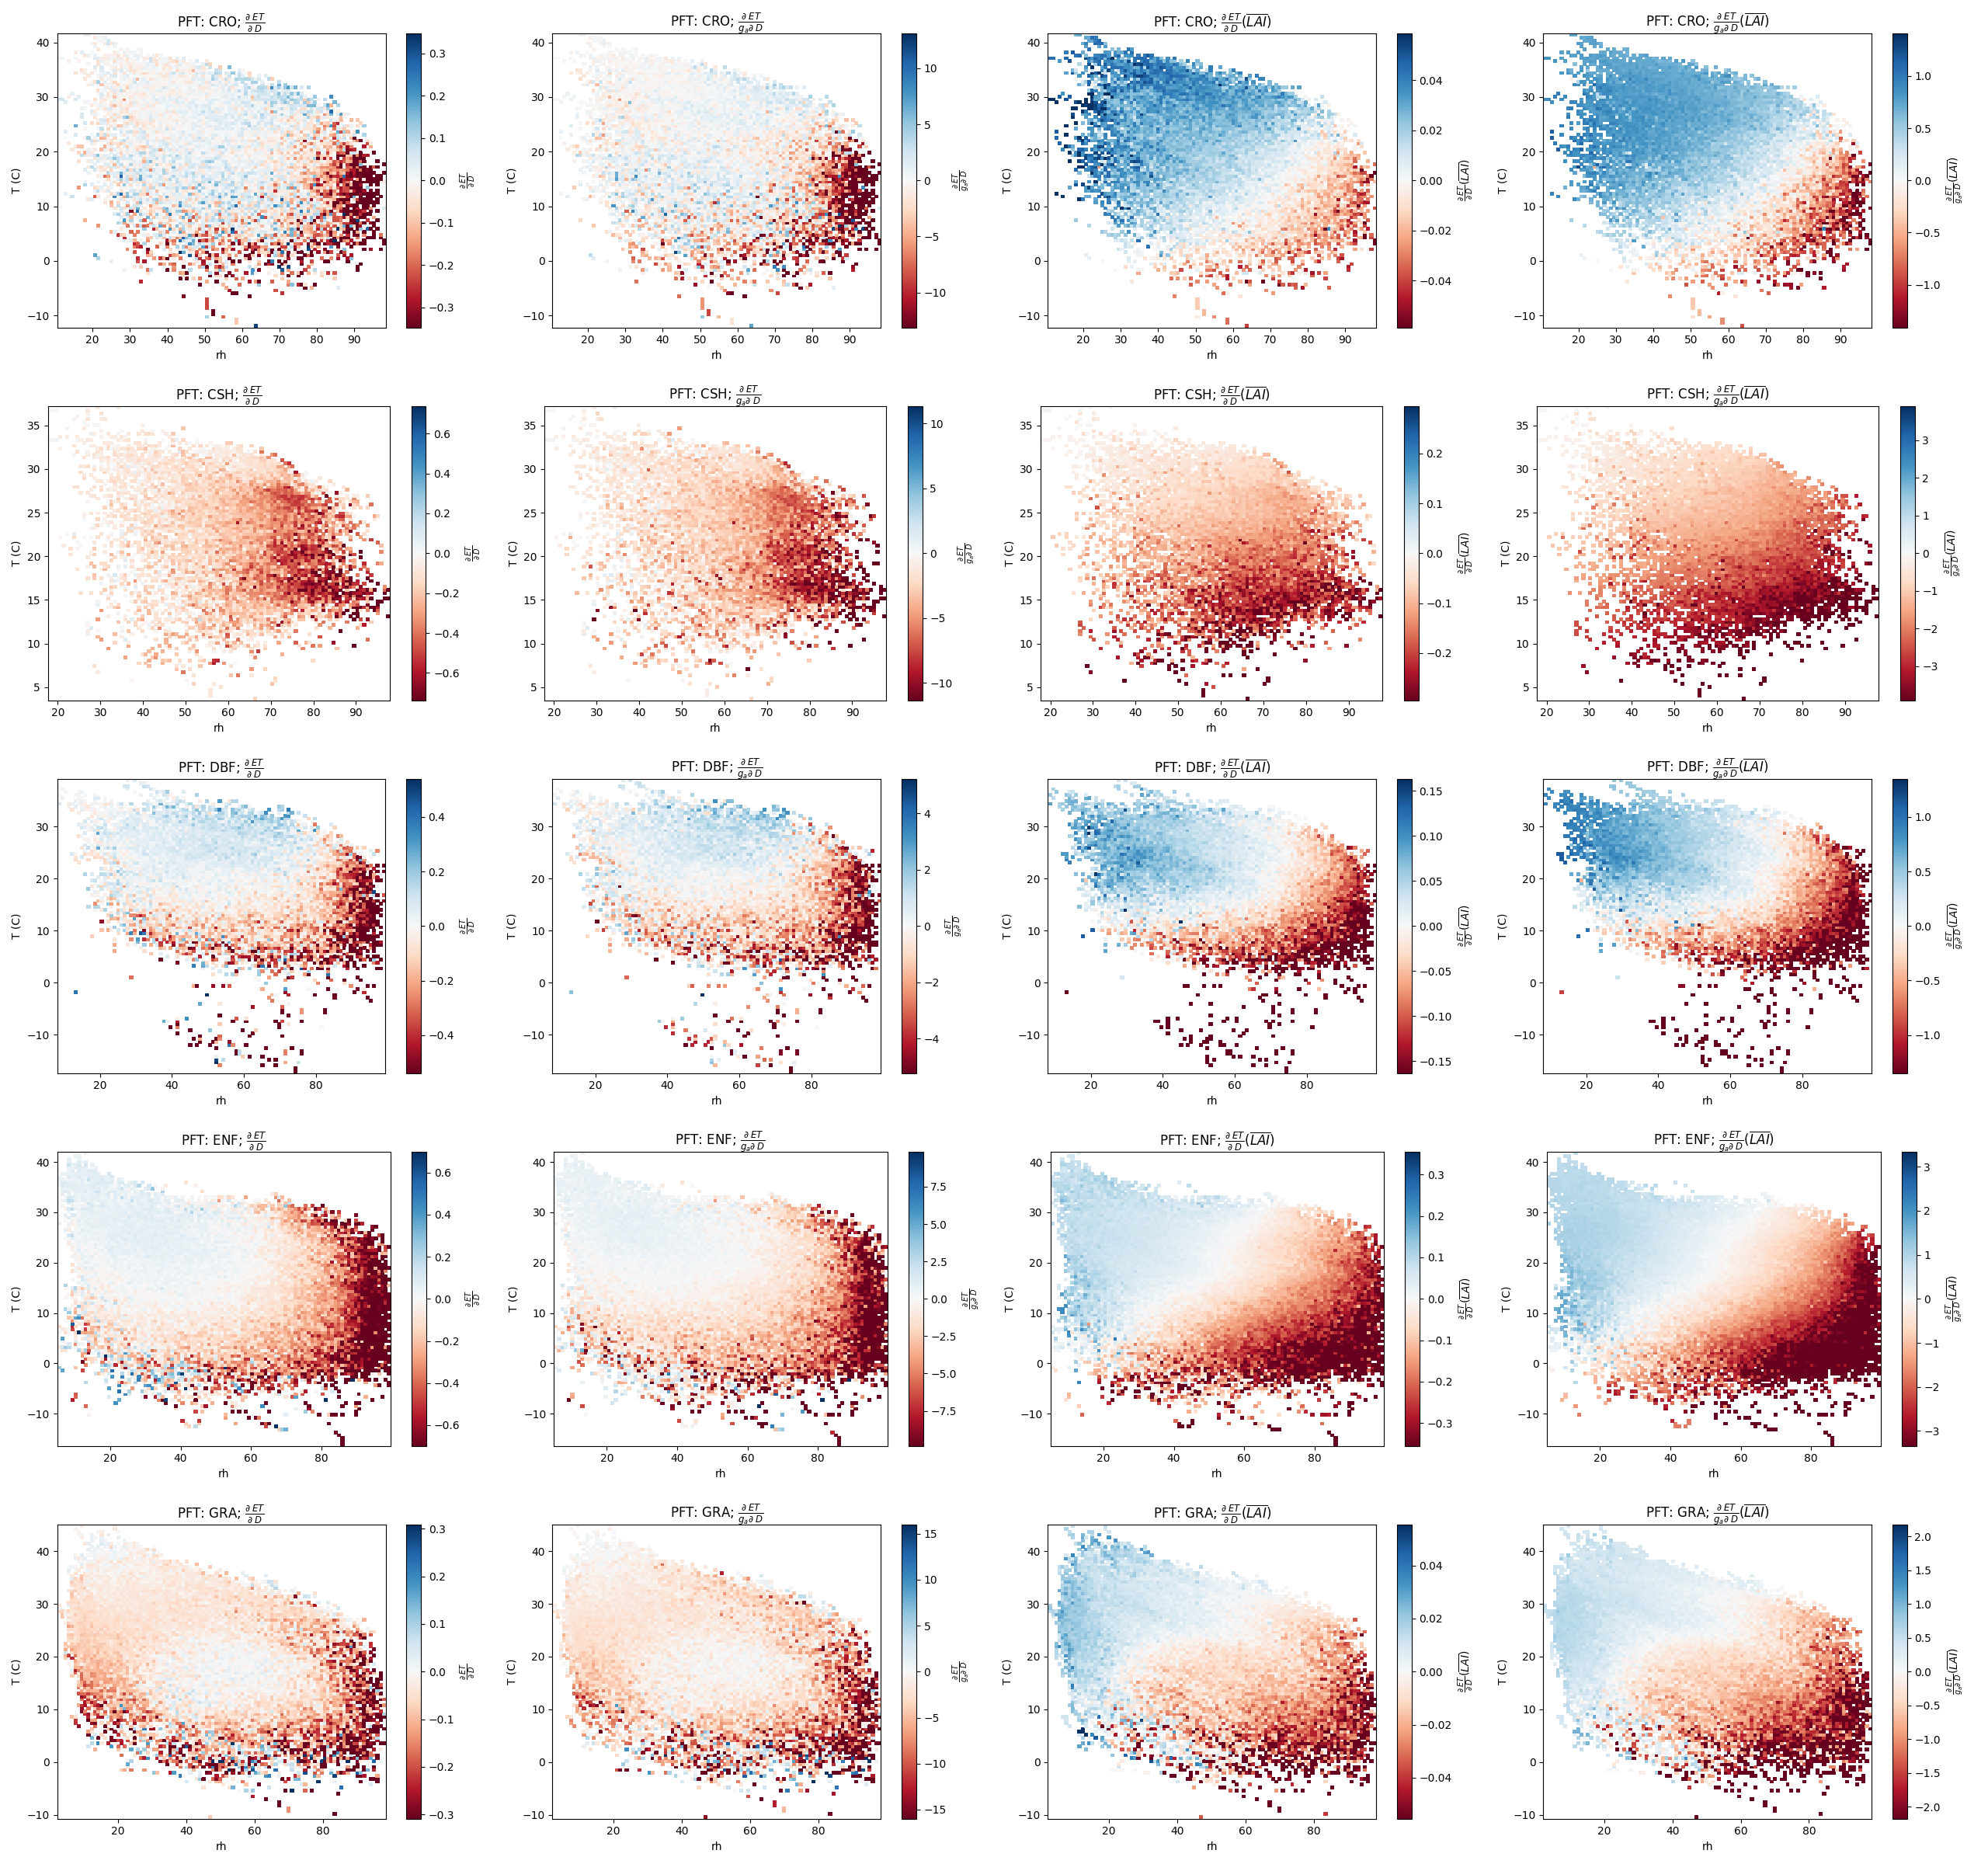
\includegraphics[width=\textwidth]{./fig06b.png}
% \caption{****alternate Fig 06****  Scatter plots of $\frac{\partial \; ET}{\partial \; VPD}$. Each row is a different PFT, and each column is a different quantity related to $\frac{\partial \; ET}{\partial \; VPD}$, as labeled. If I end up using this, I could also draw on the curve of $VPD_{crit}$ with $\overline{\frac{\text{LAI}}{\text{LAI$_{ref}$}}}$. }
% \label{real2}
% \end{figure}


\section{Limitations of theory}
\explain{HERE DISCUSS LIMITATION OF THE METHODS TO BVERY DRY CONDITIONS AND THE FEEDBCAK TO THE ATMOSPHERE OF VERY DRY SOIL CONDITIONS (BERG ET AL 2016, GENTINE ET AL> 2016)}

\section{Conclusions} 

We derived a new form of Penman Monteith using $uWUE$ (\cite{Zhou_2015}) to remove the stomatal conductance term's implicit dependence on ET. With our new form of Penman Monteith we developed a theory for when an ecosystem will tend to reduce or increase ET with increasing VPD. The goal was to capture the leading order behavior of the system to gain some intrinsic knowledge for its behavior. This intuition can be used to disentangle land atmosphere feedbacks in more complicated scenarios, and will aid interpretation of observations and sophisticated models.

Our theory states that each plant type has a critical VPD below which ET will decrease (plant response dominating) and above which ET will increase (atmospheric demand dominates). We tested our theory using data from FLUXNET 2015, and found that for DBF and CSH the theory succeeds in capturing the leading order behavior. For ENF, the theory succeeds in capturing the leading order behavior for the sign of $\frac{\partial \; ET}{\partial \; VPD}$, but not for magnitude. In contrast, the model does not capture the behavior for CRO and GRA. In some ways we should have expected this, as our theory does not account for large sources of variability we would expect for those plant types, including varying surface roughness, c3 vs c4 photosynthesis, and potential differences in irrigation across sites. Given these deficiencies for CRO and GRA, we will withhold conclusions on their response to increasing VPD.

For the forest sites (DBF, ENF) the observed environmental VPD approximately straddles the critical VPD, with about half the observations below the critical VPD and half above. However for CSH the environmental VPD never exceeds the critical VPD, and even when uncertainty is included the sign of the derivative is almost always negative (93\% of observations).

While our theory predicts common occurrence of positive $\frac{\partial \; ET}{\partial \; VPD}$ (atmospheric demand dominates), the plant response is still important even when $\frac{\partial \; ET}{\partial \; VPD} > 0$. The magnitude of the ``sign term'' of our theory is always far below what it would be if we only considered the atmospheric demand term (PET). This means that any drought indices or analysis using PET will not capture how the vegetated surface respond and react to increases in atmospheric demand. However, the new uWUE-version of Penman Monteith we derived (Equation \ref{et}) could be used as a complement to PET in drought indices. One could calculate and compare indices  when plant response is ignored (PET) or included (Equation \ref{et}). 

This paper provides initial intuition for how the land surface responds to atmospheric drying. This intuition for the one-way behavior of  land surface response to atmospheric drying is critical first step to disentangling land-atmosphere feedbacks at various scales, from diurnal to seasonal and beyond. 

%%
%% Enter Figures and Tables near as possible to where they are first mentioned:
%
% DO NOT USE \psfrag or \subfigure commands.
%
% Figure captions go below the figure.
% Table titles go above tables;  other caption information
%  should be placed in last line of the table, using
% \multicolumn2l{$^a$ This is a table note.}
%
%----------------
% EXAMPLE FIGURE
%
% \begin{figure}[h]
% \centering
% when using pdflatex, use pdf file:
% \includegraphics[width=20pc]{figsamp.pdf}
%
% when using dvips, use .eps file:
% \includegraphics[width=20pc]{figsamp.eps}
%
% \caption{Short caption}
% \label{figone}
%  \end{figure}
%
% ---------------
% EXAMPLE TABLE
%
% \begin{table}
% \caption{Time of the Transition Between Phase 1 and Phase 2$^{a}$}
% \centering
% \begin{tabular}{l c}
% \hline
%  Run  & Time (min)  \\
% \hline
%   $l1$  & 260   \\
%   $l2$  & 300   \\
%   $l3$  & 340   \\
%   $h1$  & 270   \\
%   $h2$  & 250   \\
%   $h3$  & 380   \\
%   $r1$  & 370   \\
%   $r2$  & 390   \\
% \hline
% \multicolumn{2}{l}{$^{a}$Footnote text here.}
% \end{tabular}
% \end{table}

%% SIDEWAYS FIGURE and TABLE 
% AGU prefers the use of {sidewaystable} over {landscapetable} as it causes fewer problems.
%
% \begin{sidewaysfigure}
% \includegraphics[width=20pc]{figsamp}
% \caption{caption here}
% \label{newfig}
% \end{sidewaysfigure}
% 
%  \begin{sidewaystable}
%  \caption{Caption here}
% \label{tab:signif_gap_clos}
%  \begin{tabular}{ccc}
% one&two&three\\
% four&five&six
%  \end{tabular}
%  \end{sidewaystable}

%% If using numbered lines, please surround equations with \begin{linenomath*}...\end{linenomath*}
%\begin{linenomath*}
%\begin{equation}
%y|{f} \sim g(m, \sigma),
%\end{equation}
%\end{linenomath*}

%%% End of body of article

%%%%%%%%%%%%%%%%%%%%%%%%%%%%%%%%
%% Optional Appendix goes here
%
% The \appendix command resets counters and redefines section heads
%
% After typing \appendix
%
%\section{Here Is Appendix Title}
% will show
% A: Here Is Appendix Title
%
%\appendix
%\section{Here is a sample appendix}

%%%%%%%%%%%%%%%%%%%%%%%%%%%%%%%%%%%%%%%%%%%%%%%%%%%%%%%%%%%%%%%%
%
% Optional Glossary, Notation or Acronym section goes here:
%
%%%%%%%%%%%%%%  
% Glossary is only allowed in Reviews of Geophysics
%  \begin{glossary}
%  \term{Term}
%   Term Definition here
%  \term{Term}
%   Term Definition here
%  \term{Term}
%   Term Definition here
%  \end{glossary}

%
%%%%%%%%%%%%%%
% Acronyms
%   \begin{acronyms}
%   \acro{Acronym}
%   Definition here
%   \acro{EMOS}
%   Ensemble model output statistics 
%   \acro{ECMWF}
%   Centre for Medium-Range Weather Forecasts
%   \end{acronyms}

%
%%%%%%%%%%%%%%
% Notation 
%   \begin{notation}
%   \notation{$a+b$} Notation Definition here
%   \notation{$e=mc^2$} 
%   Equation in German-born physicist Albert Einstein's theory of special
%  relativity that showed that the increased relativistic mass ($m$) of a
%  body comes from the energy of motion of the body—that is, its kinetic
%  energy ($E$)—divided by the speed of light squared ($c^2$).
%   \end{notation}




%%%%%%%%%%%%%%%%%%%%%%%%%%%%%%%%%%%%%%%%%%%%%%%%%%%%%%%%%%%%%%%%
%
%  ACKNOWLEDGMENTS
%
% The acknowledgments must list:
%
% •	All funding sources related to this work from all authors
%
% •	Any real or perceived financial conflicts of interests for any
%	author
%
% •	Other affiliations for any author that may be perceived as
% 	having a conflict of interest with respect to the results of this
% 	paper.
%
% •	A statement that indicates to the reader where the data
% 	supporting the conclusions can be obtained (for example, in the
% 	references, tables, supporting information, and other databases).
%
% It is also the appropriate place to thank colleagues and other contributors. 
% AGU does not normally allow dedications.


\acknowledgments
This work used eddy covariance data acquired and shared by the FLUXNET community, including these networks: AmeriFlux, AfriFlux, AsiaFlux, CarboAfrica, CarboEuropeIP, CarboItaly, CarboMont, ChinaFlux, Fluxnet-Canada, GreenGrass, ICOS, KoFlux, LBA, NECC, OzFlux-TERN, TCOS-Siberia, and USCCC. The ERA-Interim reanalysis data are provided by ECMWF and processed by LSCE. The FLUXNET eddy covariance data processing and harmonization was carried out by the European Fluxes Database Cluster, AmeriFlux Management Project, and Fluxdata project of FLUXNET, with the support of CDIAC and ICOS Ecosystem Thematic Center, and the OzFlux, ChinaFlux and AsiaFlux offices.


%% ------------------------------------------------------------------------ %%
%% Citations

% Please use ONLY \citet and \citep for reference citations.
% DO NOT use other cite commands (e.g., \cite, \citeyear, \nocite, \citealp, etc.).


%% Example \citet and \citep:
%  ...as shown by \citet{Boug10}, \citet{Buiz07}, \citet{Fra10},
%  \citet{Ghel00}, and \citet{Leit74}. 

%  ...as shown by \citep{Boug10}, \citep{Buiz07}, \citep{Fra10},
%  \citep{Ghel00, Leit74}. 

%  ...has been shown \citep [e.g.,][]{Boug10,Buiz07,Fra10}.



%%  REFERENCE LIST AND TEXT CITATIONS
%
% Either type in your references using
%
% \begin{thebibliography}{}
% \bibitem[{\textit{Kobayashi et~al.}}(2003)]{R2013} Kobayashi, T.,
% Tran, A.~H., Nishijo, H., Ono, T., and Matsumoto, G.  (2003).
% Contribution of hippocampal place cell activity to learning and
% formation of goal-directed navigation in rats. \textit{Neuroscience}
% 117, 1025--1035.
%
% \bibitem{}
% Text
% \end{thebibliography}
%
%%%%%%%%%%%%%%%%%%%%%%%%%%%%%%%%%%%%%%%%%%%%%%%
% Or, to use BibTeX:
%
% Follow these steps
%
% 1. Type in \bibliography{<name of your .bib file>} 
%    Run LaTeX on your LaTeX file.
%
% 2. Run BiBTeX on your LaTeX file.
%
% 3. Open the new .bbl file containing the reference list and
%   copy all the contents into your LaTeX file here.
%
% 4. Run LaTeX on your new file which will produce the citations.
%
% AGU does not want a .bib or a .bbl file. Please copy in the contents of your .bbl file here.
%\bibliography{references.bib}
% 11/23/2015
\documentclass[draft,linenumbers]{agujournal}
% \draftfalse
\usepackage{makecell}
\drafttrue

\journalname{Agricultural and Forest Meteorology}

\begin{document}

%% ------------------------------------------------------------------------ %%
%  Title
% 
% (A title should be specific, informative, and brief. Use
% abbreviations only if they are defined in the abstract. Titles that
% start with general keywords then specific terms are optimized in
% searches)
%
%% ------------------------------------------------------------------------ %%

% Example: \title{This is a test title}

\title{When does vapor pressure deficit drive or reduce evapotranspiration?}

%% ------------------------------------------------------------------------ %%
%
%  AUTHORS AND AFFILIATIONS
%
%% ------------------------------------------------------------------------ %%

% Authors are individuals who have significantly contributed to the
% research and preparation of the article. Group authors are allowed, if
% each author in the group is separately identified in an appendix.)

% List authors by first name or initial followed by last name and
% separated by commas. Use \affil{} to number affiliations, and
% \thanks{} for author notes.  
% Additional author notes should be indicated with \thanks{} (for
% example, for current addresses). 

% Example: \authors{A. B. Author\affil{1}\thanks{Current address, Antartica}, B. C. Author\affil{2,3}, and D. E.
% Author\affil{3,4}\thanks{Also funded by Monsanto.}}

\authors{A. Massmann\affil{1}, P. Gentine\affil{1}, C. Lin\affil{1,2}}


% \affiliation{1}{First Affiliation}
% \affiliation{2}{Second Affiliation}
% \affiliation{3}{Third Affiliation}
% \affiliation{4}{Fourth Affiliation}

\affiliation{1}{Department of Earth and Environmental Engineering, Columbia University, New York, NY 10027}
\affiliation{2}{Department of Hydraulic Engineering, Tsinghua University, Beijing, CN}

  % (repeat as many times as is necessary)

%% Corresponding Author:
% Corresponding author mailing address and e-mail address:

% (include name and email addresses of the corresponding author.  More
% than one corresponding author is allowed in this LaTeX file and for
% publication; but only one corresponding author is allowed in our
% editorial system.)  

% Example: \correspondingauthor{First and Last Name}{email@address.edu}

\correspondingauthor{Adam Massmann}{akm2203@columbia.edu}

%% Keypoints, final entry on title page.

% Example: 
% \begin{keypoints}
% \item	List up to three key points (at least one is required)
% \item	Key Points summarize the main points and conclusions of the article
% \item	Each must be 100 characters or less with no special characters or punctuation 
% \end{keypoints}

%  List up to three key points (at least one is required)
%  Key Points summarize the main points and conclusions of the article
%  Each must be 100 characters or less with no special characters or punctuation 

\begin{keypoints}
\item = enter point 1 here = 
\item = enter point 2 here = 
\item = enter point 3 here = 
\end{keypoints}

%% ------------------------------------------------------------------------ %%
%
%  ABSTRACT
%
% A good abstract will begin with a short description of the problem
% being addressed, briefly describe the new data or analyses, then
% briefly states the main conclusion(s) and how they are supported and
% uncertainties. 
%% ------------------------------------------------------------------------ %%

%% \begin{abstract} starts the second page 

\begin{abstract}
= enter abstract here =
\end{abstract}


%% ------------------------------------------------------------------------ %%
%
%  TEXT
%
%% ------------------------------------------------------------------------ %%

%%% Suggested section heads:
% \section{Introduction}
% 
% The main text should start with an introduction. Except for short
% manuscripts (such as comments and replies), the text should be divided
% into sections, each with its own heading. 

% Headings should be sentence fragments and do not begin with a
% lowercase letter or number. Examples of good headings are:

% \section{Materials and Methods}
% Here is text on Materials and Methods.
%
% \subsection{A descriptive heading about methods}
% More about Methods.
% 
% \section{Data} (Or section title might be a descriptive heading about data)
% 
% \section{Results} (Or section title might be a descriptive heading about the
% results)
% 
% \section{Conclusions}


\section{Introduction}


Vapor pressure deficit (VPD) is expected to rise over continents in the future due to the combination of increased temperature and relative humidity drying\explain{Is increased RH conclusive and universal?- I'm not so sure... is there another citation? I don't think Byrne 2013 shows that.} \citep{Byrne_2013}.. In turn VPD modifies the atmospheric demand of evapotranspiration (ET) (Penman Monteith) but is also a stressor for stomata \citep{Leuning_1990, MEDLYN_2011}.

Answering the question ``When does vapor pressure deficit drive or reduce evapotranspiration?'' is thus motivated by two potential but opposing perspectives on the matter. The first, hydrometeorological, perspective is that higher vapor pressure deficit increases atmospheric demand for water from the land surface, and this drives an increase in evapotranspiration (ET). This perspective is particularly relevant because potential evapotranspiration (PET), which is used in many drought indices and hydrometeorological studies, only quantifies atmospheric demand effects. On the other hand, there is another perspective for vegetated surfaces. Plants' stomata have evolved to optimally regulate the exchange of water and carbon, and tend to close in response to increased atmospheric dryness \citep{Ball_1987, Leuning_1990, MEDLYN_2011}.  Therefore, an increase in VPD, in well watered soil conditions, may actually correspond to a decrease in ET because of stomatal closure. This decrease in ET would reduce and potentially cancel (in case of full closure) the effects of shifts to atmospheric demand. In other words, the  question ``When does VPD drive or reduce ET?'' can be related to whether plant regulation or atmospheric demand dominate ET. If plant response reduces ET in response to atmospheric drying then soil moisture will be better conserved. This would seem a sensible evolutionary strategy to cope with aridity. If stomata were fully passive \citep [similar to soil pores, e.g. ][]{Or_2013}, increased atmospheric aridity would further reduce soil moisture. In turn, this would further increase aridity as low soil moisture levels increase the Bowen ratio, and in turn increase temperature and reduce atmospheric humidity (gentine et al. GRL 2016, Berg 2016).  This however would not seem to be a sensible strategy for plants from an evolutionary standpoint.

First, whether VPD drives or reduces ET should be a function of plant type. Plants that evolved to conserve water (e.g. arid shrubs) will be more likely to reduce ET with increasing VPD, and plants that have evolved to care little about water (e.g. crops) will be more likely to increase ET with increasing VPD. Atmospheric conditions must matter as well. At the ecosystem scale there are limits to the strategies plants use to hold water back from the atmosphere. As atmospheric demand for water (VPD) increases, ecosystems will begin to reach their water conservation limits. At this stage any further increase in VPD will most likely drive an increase in ET, because there is little more the plants can do keep water back. 

The objective of the present manuscript is thus to evaluate the VPD dependence of ET, in non-extreme soil drought conditions. The goal of this paper is to use reasonable approximations as a tool to increase intuition for plant response to atmospheric drying. This intuition will aid interpretation of observations and full complexity models. In order to quantify plant response to perturbations in VPD, we apply a Penman-Monteith framework to derive theoretical response of ET to VPD. The model is then validated and tested at multiple eddy-covariance stations spanning various climates and plant functional types. Section 2 describes the data used. Section 3 derives the framework. Section 4 presents results and comparison to observations. Section 5 discusses conclusions. 

\section{Data}
\label{data}
We use both meterological and turbulent flux data from the FLUXNET2015 database, including all sites with more than four years of data\explain{Pierre says ``be as precise as possible,'' but not sure what he means}. Each site's plant functional type (PFT) was classified using the International Geosphere-Biosphere Programme vegetation classification scheme \citep{Loveland_1999}. The physical constants used in Section \ref{methods} are only published for five plant functional types (PFTs) crops (CRO), deciduous broadleaf forest (DBF), evergreen needleleaf forest (ENF), grass (GRA), and closed shrub (CSH) (see Table \ref{pft}). There are 56 sites with these plant functional types, and their location is shown in  Figure \ref{map_fig} \explain{map needs to be improved - it's a placeholder for now}.

The purpose of this study is to examine ecosystem response to atmospheric drying during the growing season. To accomplish this, we filter and quality control the data using a similar procedure as \cite{Zhou_2015}:
\begin{itemize}
\item Only measured or highest (``good'') quality gapfilled data, according to quality control flags, are used.
\item To isolate the growing season, we only use days in which the average GPP exceeds 10\% of the observed 95th percentile of GPP for a given site. GPP is calculated using the nighttime respiration partitioning method.
\item We remove days with rain and the day following to avoid issues with rain interception and sensor saturation at high relative humidity (\cite{MEDLYN_2011}).
\end{itemize}
Additionally, we restrict data to the daytime, which is identified when downwelling shortwave radiation is greater than 50 W m$^{-2}$ and sensible heat flux is greater than 5 W m$^{-2}$. To further reduce the chance of sensor saturation at high relative humidity, we remove all time steps for which VPD is less than .01 kPa. Timesteps with negative observed GPP or ET are also removed, and we aggregate half hourly data to hourly averages to reduce noise. After these quality control procedures, 332556 upscaled hourly observations remain. 

\section{Methods}
\label{methods}
The Penman-Monteith equation (hereafter PM \explain{find pm ciatation in shuttlewroth}) estimates ET as a function of observable atmospheric variables and surface conductances:
\begin{linenomath*}
  \begin{equation}
      ET = \frac{\Delta R + g_a \rho_a c_p VPD}{\Delta + \gamma(1 + \frac{g_a}{g_s})},
  \end{equation}
\end{linenomath*}
where variable definitions are given in Table 1. \citet{MEDLYN_2011} developed a model for stomatal conductance ($g_s$) by combining optimal photosynthesis theory \citep{Farquhar_1980, Katul_2010} with empirical approaches, which describes the dependence of $g_s$ to VPD. The result for leaf-scale stomatal conductance was:

\begin{linenomath*}
  \begin{equation}
  g_{l-s} = g_0 + 1.6 \left(1 + \frac{g_1}{\sqrt{VPD}}\right) \frac{A}{c_s}
  \end{equation}
\end{linenomath*}
This model has been shown to behave very well across PFTs, compared to other models \citep{Lin_2015}.

This can be adapted to the ecosystem scale by multiplying by leaf area index (LAI) and converting units to m s$^{-1}$:

\begin{linenomath*}
  \label{medlyn}
  \begin{equation}
  g_s = \text{LAI} \frac{R \,T}{P} \left( g_0 + 1.6 \left(1 + \frac{g_1}{\sqrt{VPD}}\right) \frac{A}{c_s}\right)
  \end{equation}
\end{linenomath*}

While Equation 3 can be used in PM (equation 1), it will make analytical work with the function intractable because $A$, net CO$_2$ assimilation, is functionally related to ET itself. To remove the dependence of ET on $A$ we can use the semi-empirical results of \citet{Zhou_2015}. \citet{Zhou_2015} showed that the underlying Water Use Efficiency $uWUE$:

\begin{linenomath*}
  \begin{equation}
    \label{uwue}
uWUE = \frac{GPP \cdot \sqrt{VPD}}{ET}
  \end{equation}
\end{linenomath*}
is relatively constant across time and space (within plant functional type). If, following \citet{Lin_2015}, we approximate $g_0$ as $0$ (i.e. we neglect cuticular and epidermal losses - a reasonable assumption except in very dry conditions), we can use uWUE to remove $A$ from $g_s$ in a way that makes PM analytically tractable:

\begin{linenomath*}
  \begin{equation}
  g_s = \frac{R \, T}{P} 1.6 \left(1 + \frac{g_1}{\sqrt{VPD}}\right) \frac{uWUE \; ET}{c_s \; \sqrt{VPD}}
  \end{equation}
\end{linenomath*}

Note that $uWUE$ is fit on the ecosystem scale in \citet{Zhou_2015} so GPP in \ref{uwue} is really $A\cdot \text{LAI}$. This leads to the cancelation of LAI in addition to uWUE in Equation \ref{medlyn}. Plugging Equation 5 into Equation 1 and rearranging gives a new expression for ET directly as a function of VPD:

\begin{linenomath*}
  \begin{equation}
    ET = \frac{\Delta R + \frac{g_a\; P}{T} \left( \frac{ c_p VPD}{R_{air}} -  \frac{\gamma c_s \sqrt{VPD} }{ R* \; 1.6\; \text{ uWUE } (1 + \frac{g_1}{\sqrt{VPD}})} \right) }{ \Delta + \gamma}
    \label{et}
  \end{equation}
\end{linenomath*}

Given FLUXNET data described in Section \ref{data}, every term in Equation \ref{et} is known. However, our sampling of sites at the global scale may introduce some deviations of $uWUE$ from those observed in \citet{Zhou_2015}. Also, we wish to include some measure of uncertainty in our analysis to check whether our assumptions and simplifications are reasonable. To account for both mean deviations of $uWUE$ and uncertainty, we will introduce an uncertainty parameter $\sigma$ modifying $uWUE$:

\begin{linenomath*}
  \begin{equation}
    ET = \frac{\Delta R + \frac{g_a\; P}{T} \left( \frac{ c_p VPD}{R_{air}} -  \frac{\gamma c_s \sqrt{VPD} }{ R* \; 1.6\; \sigma \; \text{ uWUE } (1 + \frac{g_1}{\sqrt{VPD}})} \right) }{ \Delta + \gamma}
    \label{et_sigma}
  \end{equation}
\end{linenomath*}

Now, from each FLUXNET observation we can evaluate $\sigma$ at each time step and thus we can evaluate departure from our theory (as a departure from unity). The variability of $\sigma$ across sites and time provides a measure of uncertainty in our model, assumptions, as well as the FLUXNET observations themselves. To correct for differences in sampling between \cite{Zhou_2015} and our data, we set uWUE such that $\overline{\sigma} = 1$. The variability of $\sigma$ then propagates through any uncertainty to our derivative of Equation \ref{et_sigma}:

\begin{linenomath*}
  \begin{equation}
    \frac{\partial \;  ET}{\partial \; VPD} = \frac{2\; g_a \; P}{T(\Delta + \gamma)}   \left(\frac{ c_p}{R_{air}} -  \frac{\gamma c_s }{1.6 \; R*\; \sigma \; \text{ uWUE }} \left( \frac{2 g_1 + \sqrt{VPD}}{2 (g_1 + \sqrt{VPD})^2}\right) \right)
    \label{d_et}
  \end{equation}
\end{linenomath*}

With Equation \ref{d_et} we have provided an analytical framework for ecosystem response to atmospheric demand perturbations. There are a few subtleties to taking the derivative in Equation \ref{d_et}: $\Delta$ ($\frac{d e_{s}}{d T}$) and $VPD$ are functionally related, so while taking the derivative we evaluate $\frac{\partial \; ET}{\partial \; VPD} = \frac{\partial \; ET} {\partial \; e_s} \frac{\partial \; e_s}{\partial \; VPD} \Big|_{\text{RH fixed}} + \frac{\partial \; ET}{\partial \; RH} \frac{\partial \; RH}{\partial \; VPD} \Big|_{\text{$e_s$ fixed}}$. $RH$ and $e_s$ are assumed to be approximately orthogonal. 

We note one final comment on our derivation which is relevant for future analysis. If we  approximate $c_s$ at a global mean CO$_2$ concentration, then the RHS of Equation \ref{et} is fully defined using commonly available weather station data and the constants published in \citet{Zhou_2015, Lin_2015}. This makes Equation \ref{et} a useful alternative to PET in drought indices and hydrometeorological analysis for vegetated surfaces. Equation \ref{et} better reflects the physics of water exchange at the land surface. 

\begin{table}
\caption{Definition of symbols and variables, with citation for calculation if applicable.}
\centering
\begin{tabular}{l c c c}
\hline
 Variable & Description & Units & Citation \\
\hline
$e_s$  & saturation vapor pressure & Pa  & - \\ 
$T$  & temperature  & K & - \\
$\Delta$  & $\frac{\partial e_s}{\partial T}$ & Pa K$^{-1}$ & - \\
$R$  & net radiation at land surface minus ground heat flux & W m$^{-2}$   & - \\
  $g_a$  & aerodynamic conductance & m s$^{-1}$  & \makecell{\cite{Thom_1977} \\ \cite{Paulson_1970} \\ \cite{Beljaars_1991}} \\
  $\rho_a$  & air density & kg m$^{-3}$  & - \\
  $c_p$  & specific heat capacity of air at constant pressure & J K$^{-1}$ kg$^{-1}$ & - \\
  $VPD$  & vapor pressure deficit & Pa  & - \\
  $\gamma$  & psychometric constant & Pa K$^{-1}$   & - \\
  $g_s$  & stomatal conductance & m s$^{-1}$  & \cite{MEDLYN_2011} \\
  $g_{l-s}$  & leaf-scale stomatal conductance & mol m$^{-2}$ s$^{-1}$  & \cite{MEDLYN_2011} \\
  $R*$ & universal gas constant & J mol$^{-1}$ K$^{-1}$ & - \\
  $LAI$ & leaf area index & -& - \\
  $\sigma$ & uncertainty parameter & -& - \\
  $c_s$ & surface CO$_2$ concentration & $\mu$ mol CO$_2$ mol$^{-1}$ air& - \\
\hline
\multicolumn{2}{l}{$^{a}$Footnote text here.}
\end{tabular}
\end{table}

\begin{table}
  \label{pft}
\caption{Plant functional types, their abbreviation, Medlyn coefficient \citep[from ][]{Lin_2015}, and uWUE \citep[from ][]{Zhou_2015}. Note that units are converted such that the quantities fit into Equations 1-8 with the variables in Table 1.}
\centering
\begin{tabular}{l c c c}
  \hline
  Abbreviation & PFT & $g_1$ (Pa$^{0.5}$) & uWUE ($\mu$-mol [C] Pa$^{0.5}$ J$^{-1}$ [ET])  \\
  \hline
  CRO & cropland & 183.1 & 3.80 \\
  CSH & closed shrub & 148.6 & 2.18 \\
  DBF & deciduous broadleaf forest & 140.7 & 3.12 \\
  ENF & evergreen needleleaf forest & 74.3 & 3.30 \\
  GRA & grassland (C3) & 166.0 & 2.68 \\
\hline
\multicolumn{2}{l}{$^{a}$Footnote text here.}
\end{tabular}
\end{table}

\begin{figure}[h]
\centering
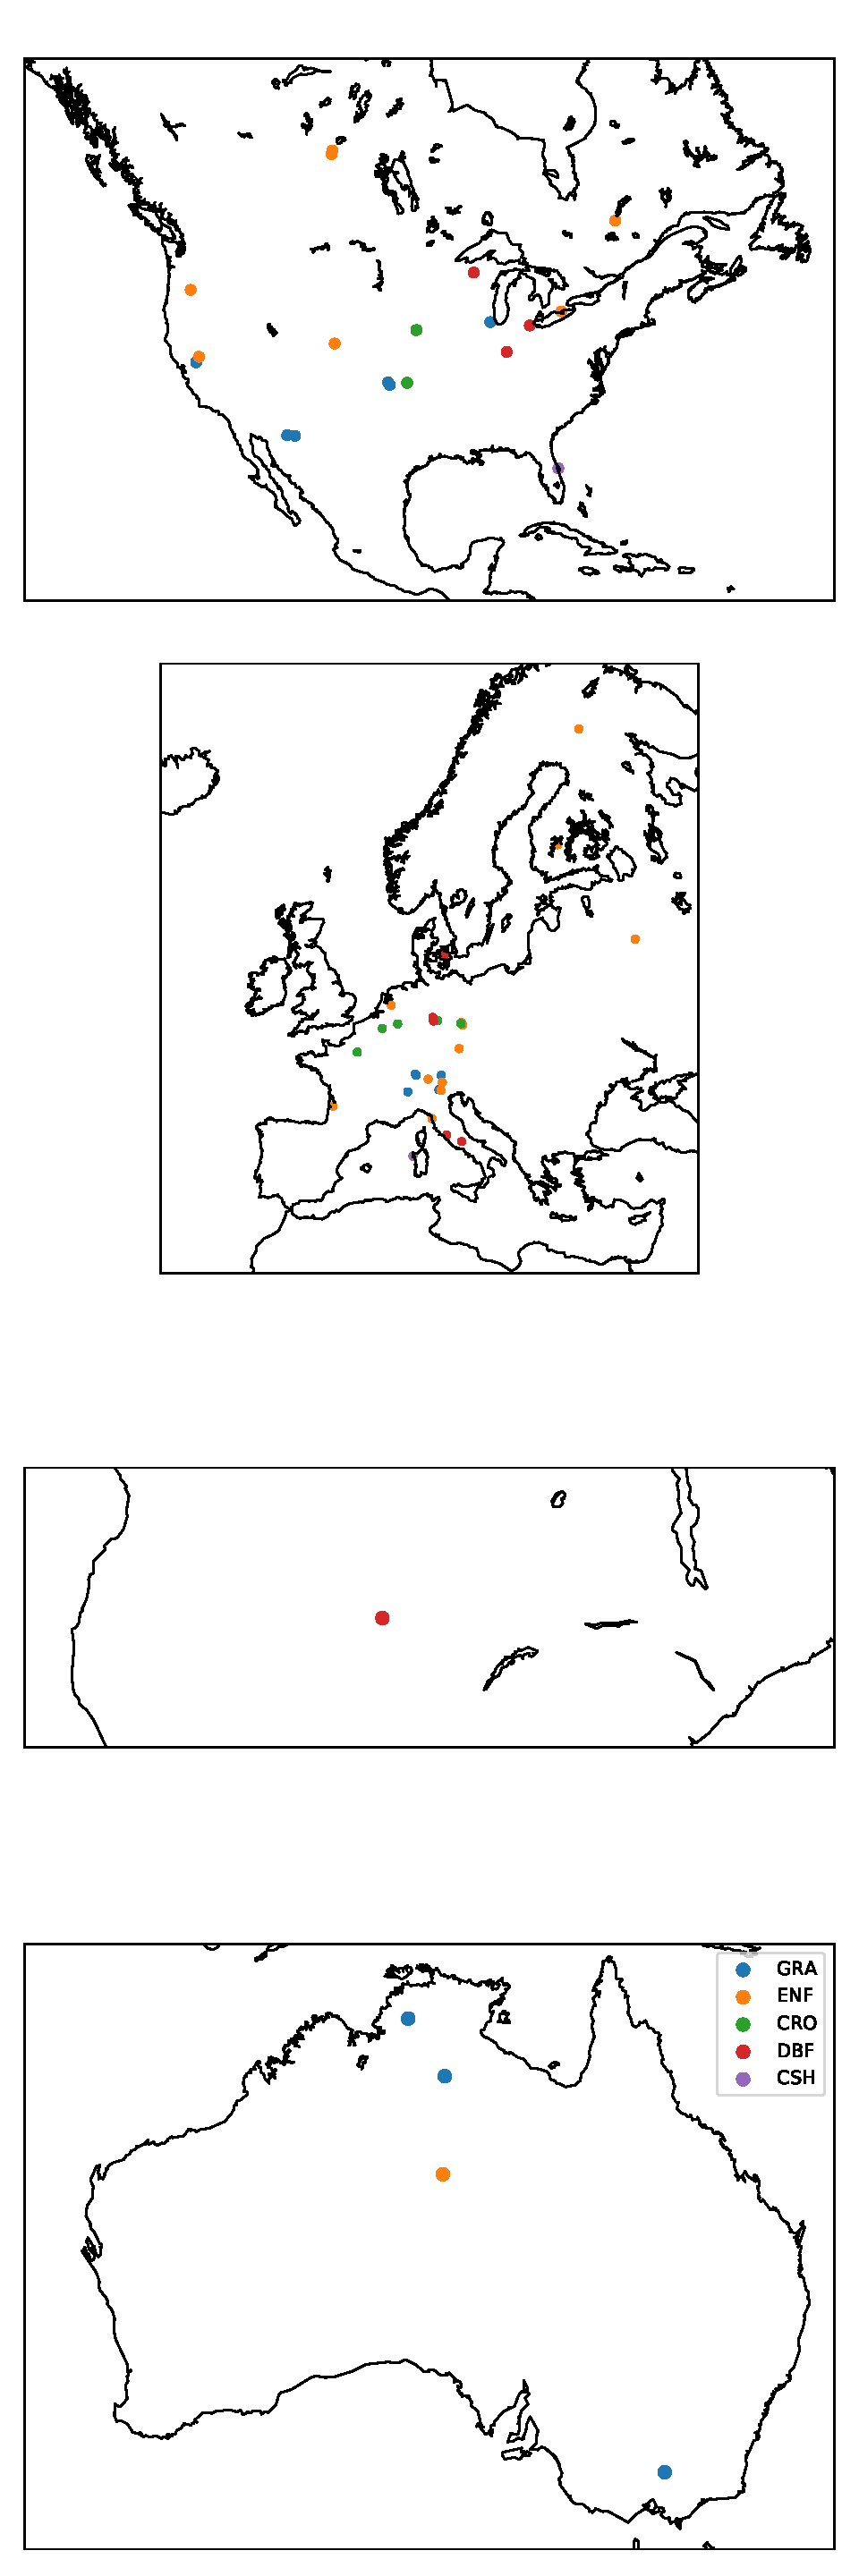
\includegraphics[width=20pc]{./fig01.pdf}
\caption{Plant functional type and location of sites used in analysis. ***\textbf{This is just  a placeholder for now, I am currently fixing it***}}
\label{map_fig}
 \end{figure}

\section{Results}
\label{results}

By construction, the variability in the $\sigma$ term (Equation \ref{sigma}) contains all model and observational uncertainties. For an observation that perfectly matches our model and constant uWUE assumption $\sigma$ will be one. Therefore, for our assumptions and framework to be reasonable $\sigma$ should be $O(1)$. Figure \ref{lai_fig} presents the histogram of calculated $\sigma$s with outliers removed (lowest and highest 5\% percent). All remaining $\sigma$ values are close to unity ($O(1)$) which provides confidence in model framework.

\begin{figure}[h]
\centering
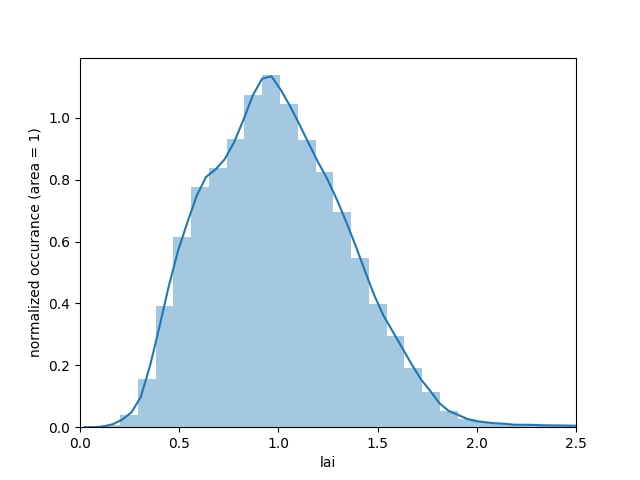
\includegraphics[width=20pc]{./fig02.png}
\caption{Histogram of $\sigma$ values calculated for each site and time according to Equation \ref{sigma}. The lowest and highest 5\% are removed as outliers, as well as any values below 0. The curve is normalized such that its area is 1. }
\label{lai_fig}
\end{figure}

An additional concern is that $\sigma$ may in fact be correlated with $VPD$, in which case the dependence would need to be accounted for when taking the derivative. Figure \ref{lai_vpd_fig} plots the joint distribution of $\sigma$ and VPD, and shows that $\sigma$ is very weakly a function of VPD. Given this weak dependence, we argue that Equation \ref{d_et} is a valid approximation for ET response to $VPD$.

\begin{figure}[h]
\centering
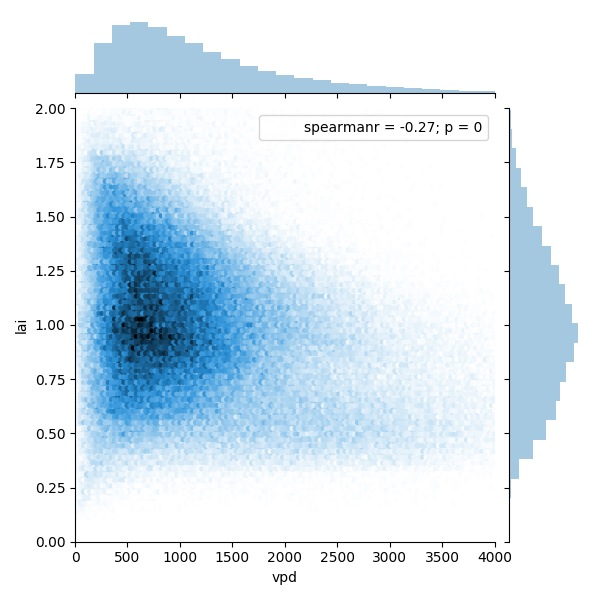
\includegraphics[width=20pc]{./fig03.png}
\caption{The joint distribution of $VPD$ and $\sigma$. $\sigma$ has only a weak dependence on $VPD$. \textbf{***note I am redoing/cleaning up this plot, ``lai'' should read sigma***}}
\label{lai_vpd_fig}
\end{figure}

Before calculating the sensitivity of ET to VPD, we will consider the functional form of Equation \ref{d_et}. There are two main terms: a ``scaling'' term, which modifies the magnitude but not the sign of the derivative $\partial ET/\partial VPD$:

\begin{equation}
  \frac{g_a \; P}{T(\Delta + \gamma)},
\end{equation}

and a ``sign'' term, which determines whether the derivative is positive i.e. atmospheric demand driven or negative i.e. physiologically controlled:

\begin{equation}
  \label{sign}
  \frac{c_p}{R_{air}} - \frac{\gamma c_s }{1.6 \; R\; \text{ uWUE }} \left( \frac{2 g_1 + \sqrt{VPD}}{2 (g_1 + \sqrt{VPD})^2}\right).
\end{equation}
All variables are positive, so the relative magnitude between the first term and the second term in Equation \ref{sign} will determine whether ET increases or decreases with increasing VPD. If the second term is larger magnitude then plant response dominates, while if the first term is larger then atmospheric demand dominates. The sign will determine whether ET is increasing or decreasing and we thus evaluate its functional form first. 

\subsection{Functional Form of the Sign Term}
\label{sign_func}
First, we explore the variables within the sign term to gain better intuition on the driver of either the increase or reduction of ET with VPD. $c_s$ and $\gamma$ are relatively constant to a good approximation so that the variability is dominated by $\sigma$ and $VPD$. $uWUE$ could vary with soil moisture but has been shown to be relatively constant except in very dry soil conditions \citep{Zhou_2016, Lin_2015}. We thus further assume that the soil is not too dry so that $uWUE$ can be approximated as a constant. This then means that the sign term only depends on VPD for a given PFT and is approximately just a function of $VPD$. We can further determine a critical threshold separating an increase from decrease in ET, such that $VPD_{crit}$ where $\frac{\partial \; ET}{\partial \; VPD} = 0$:

\begin{linenomath*}
  \begin{equation}
VPD_{crit} = \frac{R_{air}}{4 c_p} \left( \frac{\gamma c_s}{1.6\; R \; \overline{\sigma} uWUE} + \sqrt{\frac{\gamma c_s}{1.6\; R \; \overline{\sigma} uWUE}\left( \frac{\gamma c_s}{1.6\; R \; \overline{\sigma} uWUE} + 8 g_1 \frac{c_p}{R_{air}}\right)} - 4 g_1 \frac{c_p}{R_{air}} \right)
\label{vpd_min_et}
  \end{equation}
\end{linenomath*}

Values of $VPD_{crit}$ as a function of PFT are shown in Table \ref{vpd_crit}. For any values of $VPD$ less than $VPD_{crit}$, $\frac{\partial \; ET}{\partial \; VPD}$ will be negative, and for values of $VPD$ greater than $VPD_{crit}$, $\frac{\partial \; ET}{\partial \; VPD}$ will be positive. In other words, ecosystems can regulate and mitigate evaporative losses up to a VPD limit, above which atmospheric demand is just too high to be entirely compensated by stomatal regulation. We note however that even though ET increases again above the critical threshold, $VPD_{crit}$, ET is still much lower that potential evaporation as stomata are stills strongly regulating vapor fluxes. Even in the absence of soil pore evaporation, stomata do not shut down entirely at very high VPD and ET does not go to zero, because stomata are still slightly open to perform some photosynthesis \citep{Ball_1987, Leuning_1990, Medlyn_2011}. In addition, upward xylem transport is necessary to maintain phloem transport and thus carbon allocation (MENCUCCINI) \explain{Not sure citation  - Comparative criteria for models of the vasuclar transport systems of tall trees}.

\begin{table}
  \label{vpd_crit}
\caption{Values of $VPD_{crit}$, where $\frac{\partial \; ET}{\partial \; VPD} = 0$, evaluated at PFT average values for $R_{air}$, $\sigma$, $\gamma$, and $c_s$. For reference, these values are also provided CITE TABLE. For values of $VPD$ less than $VPD_{crit}$, $\frac{\partial \; ET}{\partial \; VPD}$ will be negative, and for values of $VPD$ greater than $VPD_{crit}$, $\frac{\partial \; ET}{\partial \; VPD}$ will be positive. \textbf{**** this statistics are dated, need to update***}}
\centering
\begin{tabular}{l c c c c c c}
  \hline
  PFT & $R_{air}$ & $c_s$ (ppm) & $\gamma$ &  uWUE    & \textbf{$VPD_{crit}$ (Pa)} \\
  \hline
  CRO &  288.680920 & 372.567691& 65.351523& 2.602873&  \textbf{133.165438} \\
  CSH &   289.067152& 381.593622& 67.613172& 2.175278& \textbf{4439.564212} \\
  DBF &   288.624437& 377.449849& 63.421812& 2.746393&  \textbf{888.773243} \\
  ENF &  288.183849& 377.676463& 61.559242& 4.015362&  \textbf{978.084845} \\
  GRA &  288.425651& 377.264645& 61.598768& 2.281074& \textbf{1141.630778} \\
\hline
\multicolumn{2}{l}{$^{a}$Footnote text here.}
\end{tabular}
\end{table}

Differences in $uWUE$ and $g_1$ between PFTs alter the functional form of the sign term.  Larger $uWUE$ and $g_1$ will shift the sign term towards overall positive values. $g_1$ additionally plays a primary role in determining dependnece on VPD: the smaller $g_1$, the greater the $VPD$ dependence for the PFT (Figure \ref{term3}).

Based on Figure \ref{term3} and Table \ref{vpd_crit}, CROs are the least water conservative and have the most positive constant offset, while CSH are the most water conservative and have the most negative constant offset in the sign term.  ENF ($g_1 = 74.31$) has by far the largest VPD dependence of response, while CRO ($g_1 = 183.1$) has the smallest VPD dependence. ENF are less willing to trade water for new growth, so the regulate water much more strongly depending on the dryness environment (VPD). CRO on the otherhand are more willing to trade water for new growth, so they regulate water relatively similiarly irregardless of the environment.
 
A primary takeaway from Figure \ref{term3}a is that according to our theory for all PFTs except for crops there is frequent occurrence of a negative (plant dominating) ET response to increases in VPD. This thus means that plants are able in most atmospheric conditions to redue ET in response to increased VPD and thus to reduce water losses. To better illustrate this, the ranges of observed environmental VPDs at the FLUXNET sites are plotted parallel to the x-axis. For CSH, VPD is always less than VPD$_{crit}$ so that the plant response dominates and empathizes the water conservative strategy of those plants. For CRO on the other, VPD is almost always higher than VPD$_{crit}$, emphasizing that those plants are water intensive and were actually engineered for photosynthesis rather than water saving. For forests and grass, whether plant response or atmospheric demand dominates is more dependent on the environment, with about half of of observed VPD less than VPD$_{crit}$, i.e. in conditions where plant response dominates. It is also important to note that even when atmospheric demand dominates, the response is still far smaller than it would be for potential evaporation i.e. atmospheric demand only, emphasizing that there is still a strong regulation of evaporative flux by stomata and though the plant xylem. The sign term in this case would just be a constant ($\frac{c_p}{R_{air}} \approx 3.5$), which is far larger than any part of the curves for any PFT. This highlights the deficiencies of PET's ability to capture land response to changes in atmospheric dryness (VPD). Plants are always regulating water exchange from the land surface, even when they reach the limits of they ability to do so. Therefore, the actual land surface reponse to a change in VPD will always me more negative than if the plants are not included in the physics (PET). However, we have assumed $\sigma$ (uncertainty) equal to one. We still need to test if inclusion of uncertainty could change our conclusions.
\begin{figure}[h]
\centering
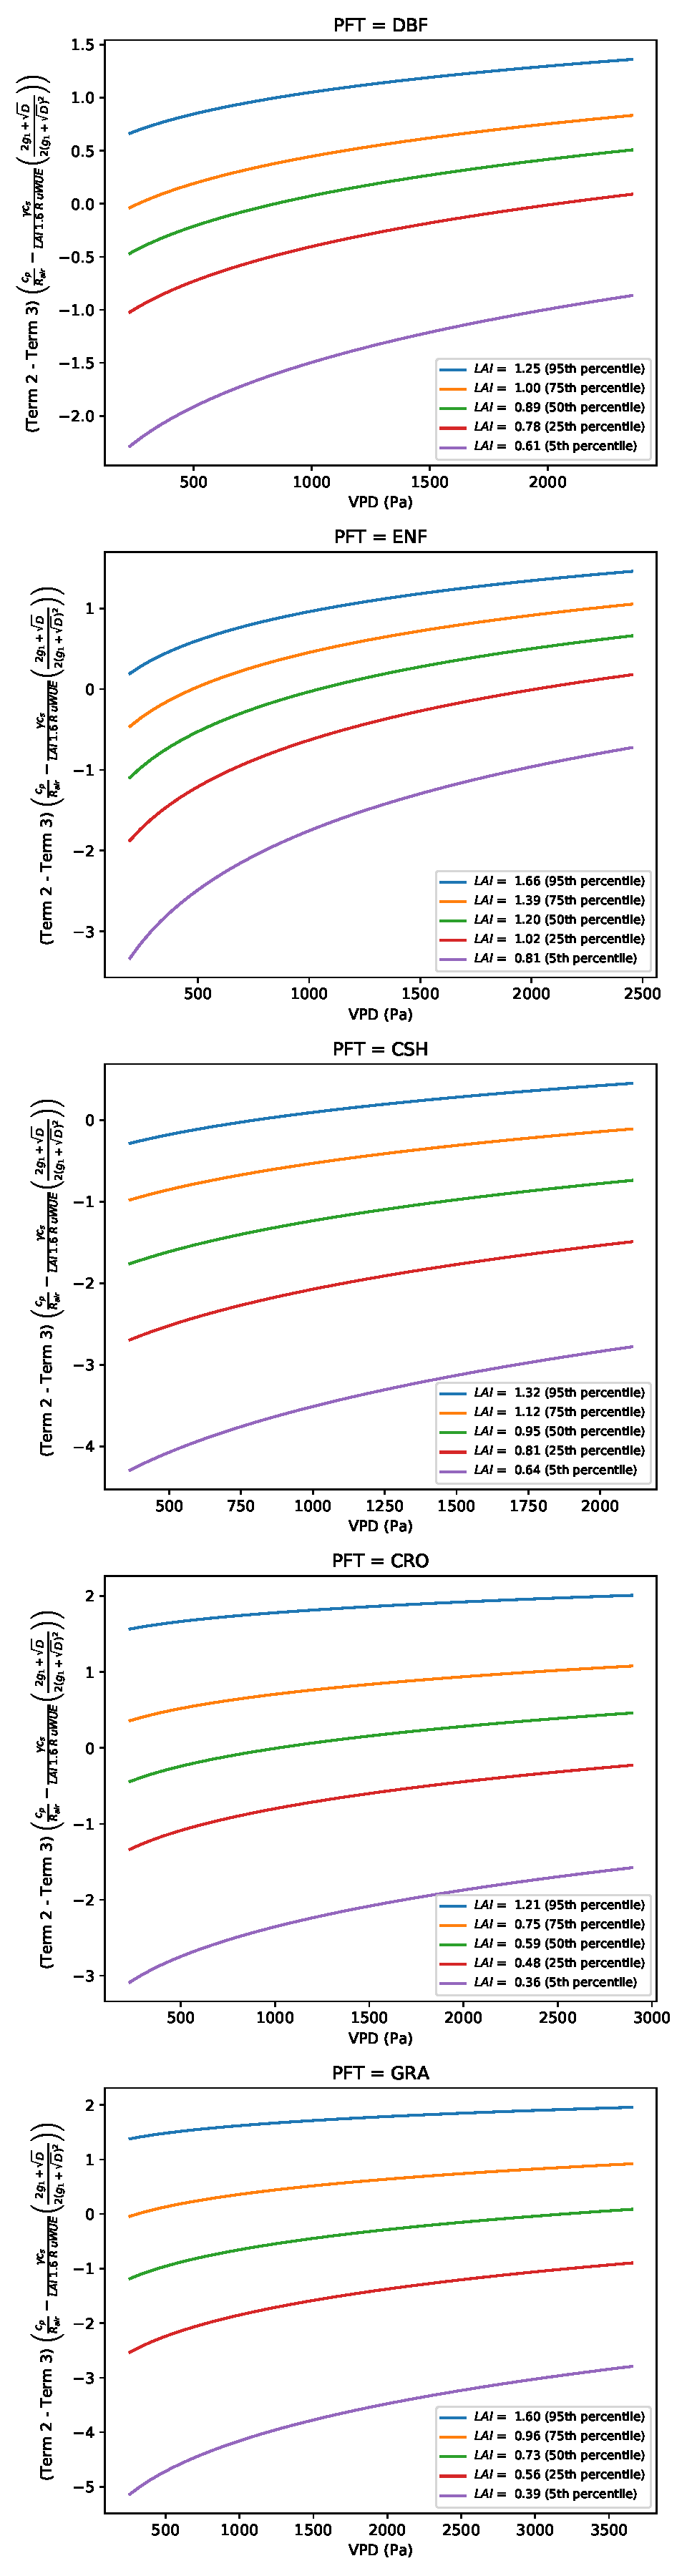
\includegraphics[width=20pc]{./fig05.pdf}
\caption{Sources of variability for the sign term. Top: sign term as a function of VPD, with $\sigma$ held fixed at 1. The observed range of VPD for each PFT is also shown below the x-axis. Line extent corresponds to 5th and 95th percentiles, while stars denote the location of the 25th, 50th, and 75th percentiles.

Bottom: The location of the minima of ET, as a function of VPD and $\sigma$. Lines and stars denote the distribution of VPD and $\sigma$ next to each axis, following the same percentiles as above. \textbf{***need to replot with correct sigma (normalized to 1), also correct uWUE label in first plot***}}
\label{term3}
\end{figure}

Figure \ref{term3}b shows the location of VPD$_{crit}$, as a function of $\sigma$ (uncertainty) and $VPD$. For any $\sigma$ or VPD less (more) than these curves, the sign term will be negative (positive). It is clear that the portion of VPD observations below/above these curves will be a strong function of $\sigma$. This motivates a thorough examination of how inclusion of uncertainty ($\sigma$) might change the form of the sign term, and in particular the location of VPD$_{crit}$ for each of our plant types. In Secion \ref{testing} we examine if and how uncertainty changes the analysis presented in this section, for each PFT.

\subsection{Functional Form of the Scaling Term}

While the above discussion of the sign of $\frac{\partial \; ET}{\partial \; VPD}$ is important to answer our research question, the magnitude of $\frac{\partial \; ET}{\partial \; VPD}$ will also the relative magnitude of the change $\frac{\partial \; ET}{\partial \; VPD}$ and the importance of $VPD$ variability for overall $ET$ variability. So we now more closely examine the scaling term: $\frac{P}{T} \propto \rho$. Air density $\rho$ scaling term varies little relative to aerodynamic conductance and $\Delta$. The psychrometric constant $\gamma$ is also relatively constant, so the scaling term should be primarily a function of aerodynamic conductance and temperature, through the slope of the Clauisu-Clapeyron relationship $\Delta$. This is as expected, given that the aerodynamic conductance represents the efficiency fo the transfer of surface anomalies to the atmosphere. As aerodynamic conductace  increases, any plant response will be communicated more strongly to the atmosphere (and vice-versa).

$\Delta$'s presence in the scaling term also matches physical intuition. Evaporative cooling will dampen the ability of the atmosphere to take more moisture, because $e_{s}$ decreases with decreasing temperature. The decrease in $e_{s}$ is proportional to $\Delta$ ($\delta e_{s} = \Delta \delta T$). So as $\Delta$ increases, you will get a larger damping of ET due to evaporative cooling.  The functional from of $\Delta$ will be the same across PFT, but the temperature range may vary slightly. In contrast, aerodynamic conductance will vary strongly with PFT due to the importance of surface roughness. So most of the differences in scaling between PFT should be in the aerodynamic conductance term. One interesting side note is that the coefficient of variability for both aerodynamic conductance and the scaling term is relatively constant across PFT, suggesting that the influence of aerodynamic conductance on the relative (to the PFT mean) variability of the scaling term is approximately similar across PFT.

Figure \ref{scale_vary}A shows the scaling term normalized by mean aerodynamic conductance (calculated for each plant functional type), and confirms that much of the relative variability of the scaling term is caused by aerodynamic conductance variability. Generally, temperature (via $\Delta$) causes less relative variability. However, the impact of $T$ on the relative variability increases with increasing aerodynamic conductance. 

While the relative variability of scaling term is similar across PFT, the absolute value of scaling term varies strongly across PFT. Figure \ref{scale_vary}B shows scaling term evaluated at the mean aerodynamic conductance for each PFT, and at the range of observed temperatures for each PFT. As expected, for the tree PFTs (DBF, ENF) the scaling term is much larger and the temperature dependence is much stronger. Systematic differences in observed temperatures also cause differences in the average magnitude of scaling term. For example, ENF experiences on average colder temperatures and is thus more likely to have a larger scaling term. Additionally, because the variability of aerodynamic conductance increases proportionally to the mean, the spread of the scaling term due to aerodynamic conductance variability will be larger for the tree PFTs, although this is not shown for simplicity. To summarize Figure \ref{scale_vary}: the variability of the scaling term within each PFT will look like Figure \ref{scale_vary}A for each PFT, but the scale of the y-axis will increase or decrease according to mean aerodynamic conductance observed in Figure \ref{scale_vary}B.
 
\begin{figure}[h]
\centering
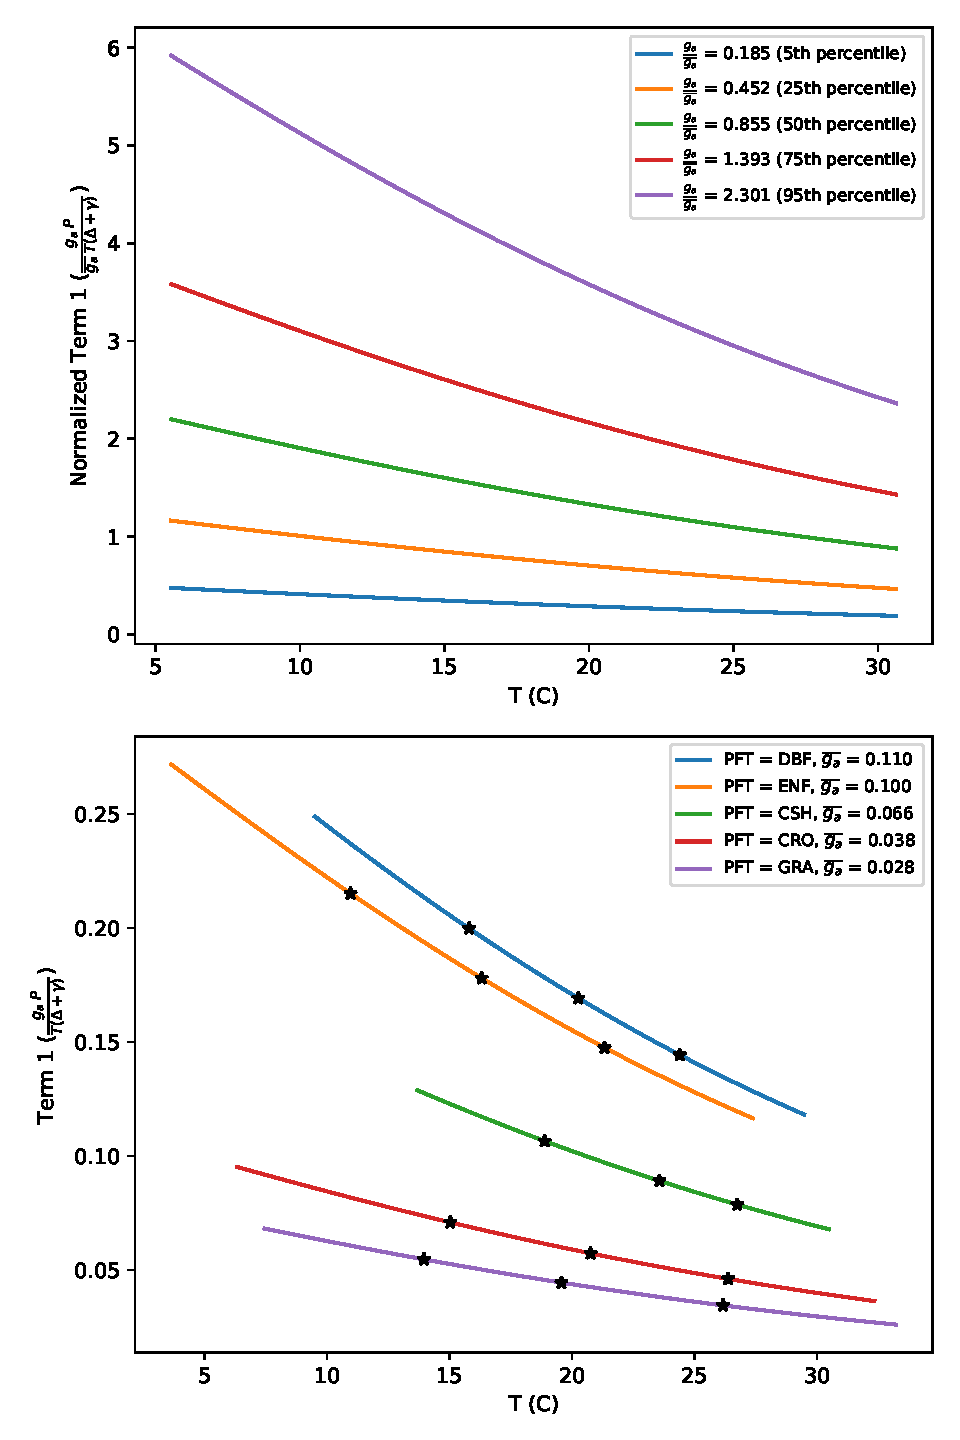
\includegraphics[width=20pc]{./fig04.pdf}
\caption{Primary sources of variability for scaling term. A) Variability within each PFT: scaling term normalized by mean $g_a$ for each PFT. B) Variability between each PFT: scaling term evaluated at mean $g_a$ for each PFT. Temperature range is 5-95th percentile for each PFT. Additionally, stars denote the location of the 25th, 50th, and 75th percentiles.}
\label{scale_vary}
\end{figure}

%%%%% replace below with idea:
\subsection{Bulk statistics of $\frac{\partial \; ET}{\partial \; VPD}$}

Table 3 confirms our expectations for PFT behavior of $\frac{\partial \; ET}{\partial \; VPD}$. For all PFTs except for CRO, average $\frac{\partial \; ET}{\partial \; VPD}$ is less than zero. However, $\frac{\partial \; ET}{\partial \; VPD}$ evaluated at the average of all variables (e.g. $\sigma$, $T$, $c_s$, $VPD$) is only negative for CSH and GRA. And, DBF in addition to CRO experiences $\frac{\partial \; ET}{\partial \; VPD}$ < 0 less than half the time. These observations highlight the effect of the nonlinear function in Figure \ref{term3}: $\frac{\partial \; ET}{\partial \; VPD}$ has a much steeper slope when the function is negative, and is thus more likely to be large magnitude.

The units of $\frac{\partial \; ET}{\partial \; VPD}$ make it difficult to interpret if $VPD$ is even a meaningful contributor to ET's variability. To better understand $VPD$'s contribution, we multiply $\frac{\partial \; ET}{\partial \; VPD}\left(\overline{env}\right)$ with $VPD$'s standard deviation to define a (linearized) relative change in ET for variations in $VPD$ . $VPD$'s contribution to ET's variability ranges between 30 - 40 W m$^{-2}$ for all PFTs except for CSH, which is about 100 W m$^{-2}$. Another meaningful comparison is to $\frac{\partial \; ET}{\partial \; R} \cdot std(R)$, as net radiation is generally the driver of ET (cite joe berry here)\explain{Find citation?}. For all PFTs except for CSH $VPD$ contributes between 30 - 40 \% of $R$'s contribution to variability. For CSH the portion is much larger, about 88 \%. $VPD$'s variability is certainly a non-negligible contributor to $ET$'s variability.

Theoretical derivation has so far illuminated the dependence of $\frac{\partial \; ET}{\partial \; VPD}$ and how it varies across PFT. Large mean $uWUE$ shifts CRO and DBF towards a tendancy to increase ET with VPD (positive $\frac{\partial \; ET}{\partial \; VPD}$), but a lower slope parameter ($g_1$) for DBF allows for decreaes in ET with VPD, at low environmental VPD. \explain{physically state how slope parameter is trade for water at leaf level, but uWUE is trade-ff between GPP and VPD at ecosystem-level}.  ENF's very low slope parameter ($g_1$), which is even lower than for DBF, increases the dependence of ET response  ($\frac{\partial \; ET}{\partial \; VPD}$) on $VPD$, and makes the function strongly nonlinear. This has the effect of making mean ET response ($\overline{\frac{\partial \; ET}{\partial \; VPD}}$)  more negative for a given frequency of occurence of negative ET response ($\frac{\partial \; ET}{\partial \; VPD} < 0$), than for other PFT. GRA shows the opposite behavior; a relatively high slope parameter ($g_1$)  makes the function more linear, causing a more positive mean ET reponse ($\overline{\frac{\partial \; ET}{\partial \; VPD}}$) for a given given frequence of negative ET reponse  ($\frac{\partial \; ET}{\partial \; VPD} < 0$). Finally, CSH's very low $uWUE$ dominates the slope parameter's effects, causing ET to almost always decrees with increasing atmospheric dryness (VPD), even with uncertainty included. Variability in $VPD$ accounts for the largest amount of $ET$ variability for CSH. For the other PFTs, $VPD$ contributes less to $ET$ variability, but still represents about 30-40 \% of $R$'s contributions to ET variability. \explain{think pierre is correct, could probably scrap this anecdote: WHAT IS THE SORUCE OF VARIBILITY OF THE REST OF ET I DON"T KNOW IF THAT IS RELEVANT FOR THE PRESENT PAPER.}

\begin{table}
\caption{Statistics of $\frac{\partial \; ET}{\partial \; VPD}$ as a function of PFT. \textbf{***dated, need to update these statistics***}}
\centering
\begin{tabular}{l c c c c c}
  \hline
PFT & $\overline{\frac{\partial \; ET}{\partial \; VPD}}$ & $\frac{\partial \; ET}{\partial \; VPD}\left(\overline{env}\right)$ & $\frac{\partial \; ET}{\partial \; VPD}\left(\overline{env}\right)*\text{std}(VPD)$ & $\frac{\frac{\partial \; ET}{\partial \; VPD}\left(\overline{env}\right)*\text{std}(VPD)}{ \frac{\partial \; ET}{\partial \; R}\left(\overline{env}\right)*\text{std}(R)}$ & fraction $\frac{\partial \; ET}{\partial \; VPD} < 0.$ \\
  \hline
CRO & 0.000853 & 0.026241 & 37.05 & 0.41 & 0.473311\\
CSH & -0.108234 & -0.091526 & 101.72 & 0.88 & 0.931660\\
DBF & -0.012727 & 0.013794 & 39.47 & 0.33 & 0.461674\\
ENF & -0.034087 & 0.000706 & 33.22 & 0.30 & 0.534425\\
GRA & -0.019637 & -0.000921 & 33.60 & 0.35 & 0.631735\\
\hline
  
\end{tabular}
\end{table}


\subsection{Validation of theory at eddy-covariance sites}
\label{testing}
So far we have developed a theory for $\frac{\partial \; ET}{\partial \; VPD}$'s behavior as a function of VPD and PFTs. We now turn to an direct evaluation against observations taken from a wide range of eddy-covariance datasets (Section \ref{methods}).

Figure \ref{agu_fig} shows the distribution of of the sign term (when uncertainty is included), as compared to what the theory would predict. Our goal was to capture the leading order behavior of the ET dependence on VPD. Given the assumptions we have made, and the uncertainties of flux tower observations themselves, we expect a large amount of noise when reprdrocuing the derivatives of ET.

For DBF our theory is successful towards this goal: the theory matches the leading order behavior of the function when uncertainty is included, and the DBG figure looks as one would expect if one just added noise on top of our theory. The VPD dependence, given by the slope parameter ($g_1$), floows the median values of each box plot. Perhaps most importantly, the x-intercept, and thus VPD$_{crit}$, matches nearly exactly between the theory and the observations. Therefor the sign of the ET response to increases in VPD should be well matched, subject to the unavoidable constraints of noise, much of which may be from the observations themselves. The uncertainty is non negligable; there are bany observations in each box for which the the sign of observation is opposite the response predicted by the theory, but to leading order our theory matches the observations. 

While CSH has a much different functional form of the sign term than DBF, CSH observations also match our theory to leading order. Again, the VPD dependence mostly determined from the slope parameter ($g_1$) closely matches the medians in the observation bins. The VPD-independent, strongly negative response, which is determined by $uWUE$, is also captured. For CSH, there is extremely rare occurence of positive ET response with VPD, even with uncertainty, so the sign of the theory almost always matches the sign of the observations, even with all of the uncertainty.

The theory does not match as well for CRO as for DBF and CSH. At low VPD the VPD dependence (due to $g_1$) is similiar to the leading order behavior of the observations, but the entire curve is shifted towards postiive values, due to some error in $uWUE$. Most strikingly, the observations show a tendency to move back towards negative values at high VPD, which given the functional form of VPD dependnce, is behavior that is impossible fo the theory to capture. This divergence between the theory and the observations for CRO could have been expected. For practical reasons, our theory does not include important sources of variability (particularly between sites) for CRO. We do not account for seasonal changes in LAI, variability in crop height and surface roughness, differences in C3 vs C4 photosynthesis, or differences in irrigation practices between the sites and/or years. This deficiencies would explain the inability of our theory to match obsercations. For example, a superpositions of sites with C3 plants (low VPD) and C4 plants (high VPD) would explain observed shift back towards negative ET reponse at high VPD when all sites are binned together, as in Figure \ref{agu_fig}.   

The theory for GRA suffers from similiar limitations as for CRO. The differences between the theory and the observations are more pronounced for GRA, but are explainable using similiar logic as that used for CRO. GRA will also have differences between sites in C3 vs C4 photosythesis, and irrigation practices, as well as strong seasonal variability in crop height and LAI. For GRA, the observations show a very different VPD dependence of response than the theory, with a strong tendency back toewards a negative ET reponse at high VPD which our theory cannot account for. As with CRO, this could be explained by a superposition of sites with C3 vs C4 sites. Unfortunately, because detailed site-level data of C3 vs C4 plant type, as well as irrigation practes, was difficult to obtain, we could not bin GRO and GRA further by irrigation and photosyethesis stragtegy. However, we hypothesize that the theory would much more closel match obsercations with photosythesis and irrigation are accounted for. 

The comparison between the theory and obsercations for ENF is unique from the rest of the PFTs. The VPD dependence of the theory, determined by the slope paramter, is not well captured by observations. However, the theory closely captures the x-intercept and VPD$_{crit}$. So, the theory still captures when the ET reponse will be positive or negative, but is less accurate with the magnitude of the reponse. Therefor the theory is still useful for addressing when VPD drives or reduces ET. Also, it's with noting that we used published constants for $g_1$ \citep[from ][]{Lin_2015}, which determines the VPD dependence. We could have fit our own constants so that the theory would best match the observations, but our goal was to use a priori physical constants whenever possible.

While the above discussion shows that our theory has some limitations when applied to some sites, especially for crops and grasslands, another question could be, how would using PET, as many hydrometeorological studies and applications do, compare with our theory.  Again, as in Section \ref{sign_func}, the PET response to changes in VPD will be constant at about 3.5. In Figure \ref{agu_fig} the ET reponse to shifts in dryness is always far more negative than 3.5 for the observations, even with all uncertainty included. So the PET reponse to atmospheric dryness is outside the range of all observable responses. This casts doubt on PET's usefulness for capturing the leading order behavior of water budgeting at the land surface. However our theory (Equation \ref{et}) could be used with published $uWUE$ and $g1$ as an alternative to PET to estimating land response and moisture budgeting.

\subsubsection{Testing VPD$_{crit}$}
As stated in the above discussion of ENF, we are mostly interested in the critical threshold $VPD_{crit}$ for which the sign of  $\frac{\partial \; ET}{\partial \; VPD}$ is determined. When $VPD < VPD_{crit}$, $\frac{\partial \; ET}{\partial \; VPD}  < 0$ (plant response dominates), and when $VPD > VPD_{crit}$, $\frac{\partial \; ET}{\partial \; VPD} > 0$ (atmospheric demand dominates). Theoretically this $VPD_{crit}$ is only a function of PFT. We can look at how this value of $VPD_{crit}$ matches the data as different observed variables (including uncertainty) are allowed to vary.


Figure \ref{real} presents calculated $\frac{\partial \; ET}{\partial \; VPD}$ where, unless otherwise noted, all variables in Equation \ref{d_et} are allowed to vary, including uncertainty. Each column represents a different quantity related to $\frac{\partial \; ET}{\partial \; VPD}$, and each row is a different PFT. Vertical black lines denote where our theory says $VPD_{crit}$ should be. For any observations to the left of this line $\frac{\partial \; ET}{\partial \; VPD}$ should be negative (plant response dominates), and any observations the right of the line should be positive (atmospheric demand dominates). In addition to seeing how our theoretically-derived VPD threshold, $VPD_{crit}$, matches observations, these analysis are also useful for observing how the scaling term affects the magnitude of the derivative, if at all. 

The scatter figures generally confirm expectations from Figure \ref{agu_fig}. By comparing different columns of Figure \ref{real} we can evaluate the impact of $\sigma$ and $g_a$ on the variability of $\frac{\partial \; ET}{\partial \; VPD}$. $g_a$'s scaling (included in columns 1 and 3) alters the magnitude considerably, particularly between PFTs. $\sigma$ variability (included in columns 1 and 2) adds a lot of additional noise to the signal of $\frac{\partial \; ET}{\partial \; VPD}$, as observed in Figure \ref{agu_fig}. However, the general story with the noise appears to match the cleaner signal when $\sigma$ is help constant and $VPD_{crit}$ is clearly visible. The exceptions are, as discussed above, for GRA and CRO, where the full complexity plots (Columns 1 and 2) do not match well with $\sigma$ held fixed (Columns 3 and 4).

While $g_a$ has a large impact on the magnitude of the scaling, temperature, through the derisive of the Clausius-Clapeyron, $\Delta$, term, does not appear to have as much of an impact in the complete estimation of $\frac{\partial \; ET}{\partial \; VPD}$. Therefore it appears that the absolute magnitude of the derivative can be mostly attributed to the sign term, and its direct scaling by aerodynamic conductance. Intuitively this is reasonable; aerodynamic conductance will control how dominant balances at the land surface are communicated to the boundary layer. While $\Delta$ controls the efficiency of latent fluxes in carrying heat away from the surface, it appears this is a second order term, relative to $g_a$, for scaling $\frac{\partial \; ET}{\partial \; VPD}$. 

In general Figures \ref{real} and \ref{agu_fig} match our expectations, even with the large sensitivity to $\sigma$ seen in Figure \ref{term3}. Our $\sigma$-based method of uncertainty propagation blurs the idealized expectations the most for GRA and CRO. We therefore have the most confidence in our conclusion based on Equation \ref{d_et} for PFTs CSH, DBF, and ENF, as the sign of the derivative with uncertainty included matches (to leading order) the story when $\sigma$ is held fixed.

\begin{figure}[h]
\centering
\includegraphics[width=\textwidth]{./agu_fig.pdf}
\caption{Comparison of the sign term with model uncertainty included (box plots) to the sign term as calculated with simplifying assumptions (blue line).}
\label{agu_fig}
\end{figure}


\begin{figure}[h]
\centering
\centerline{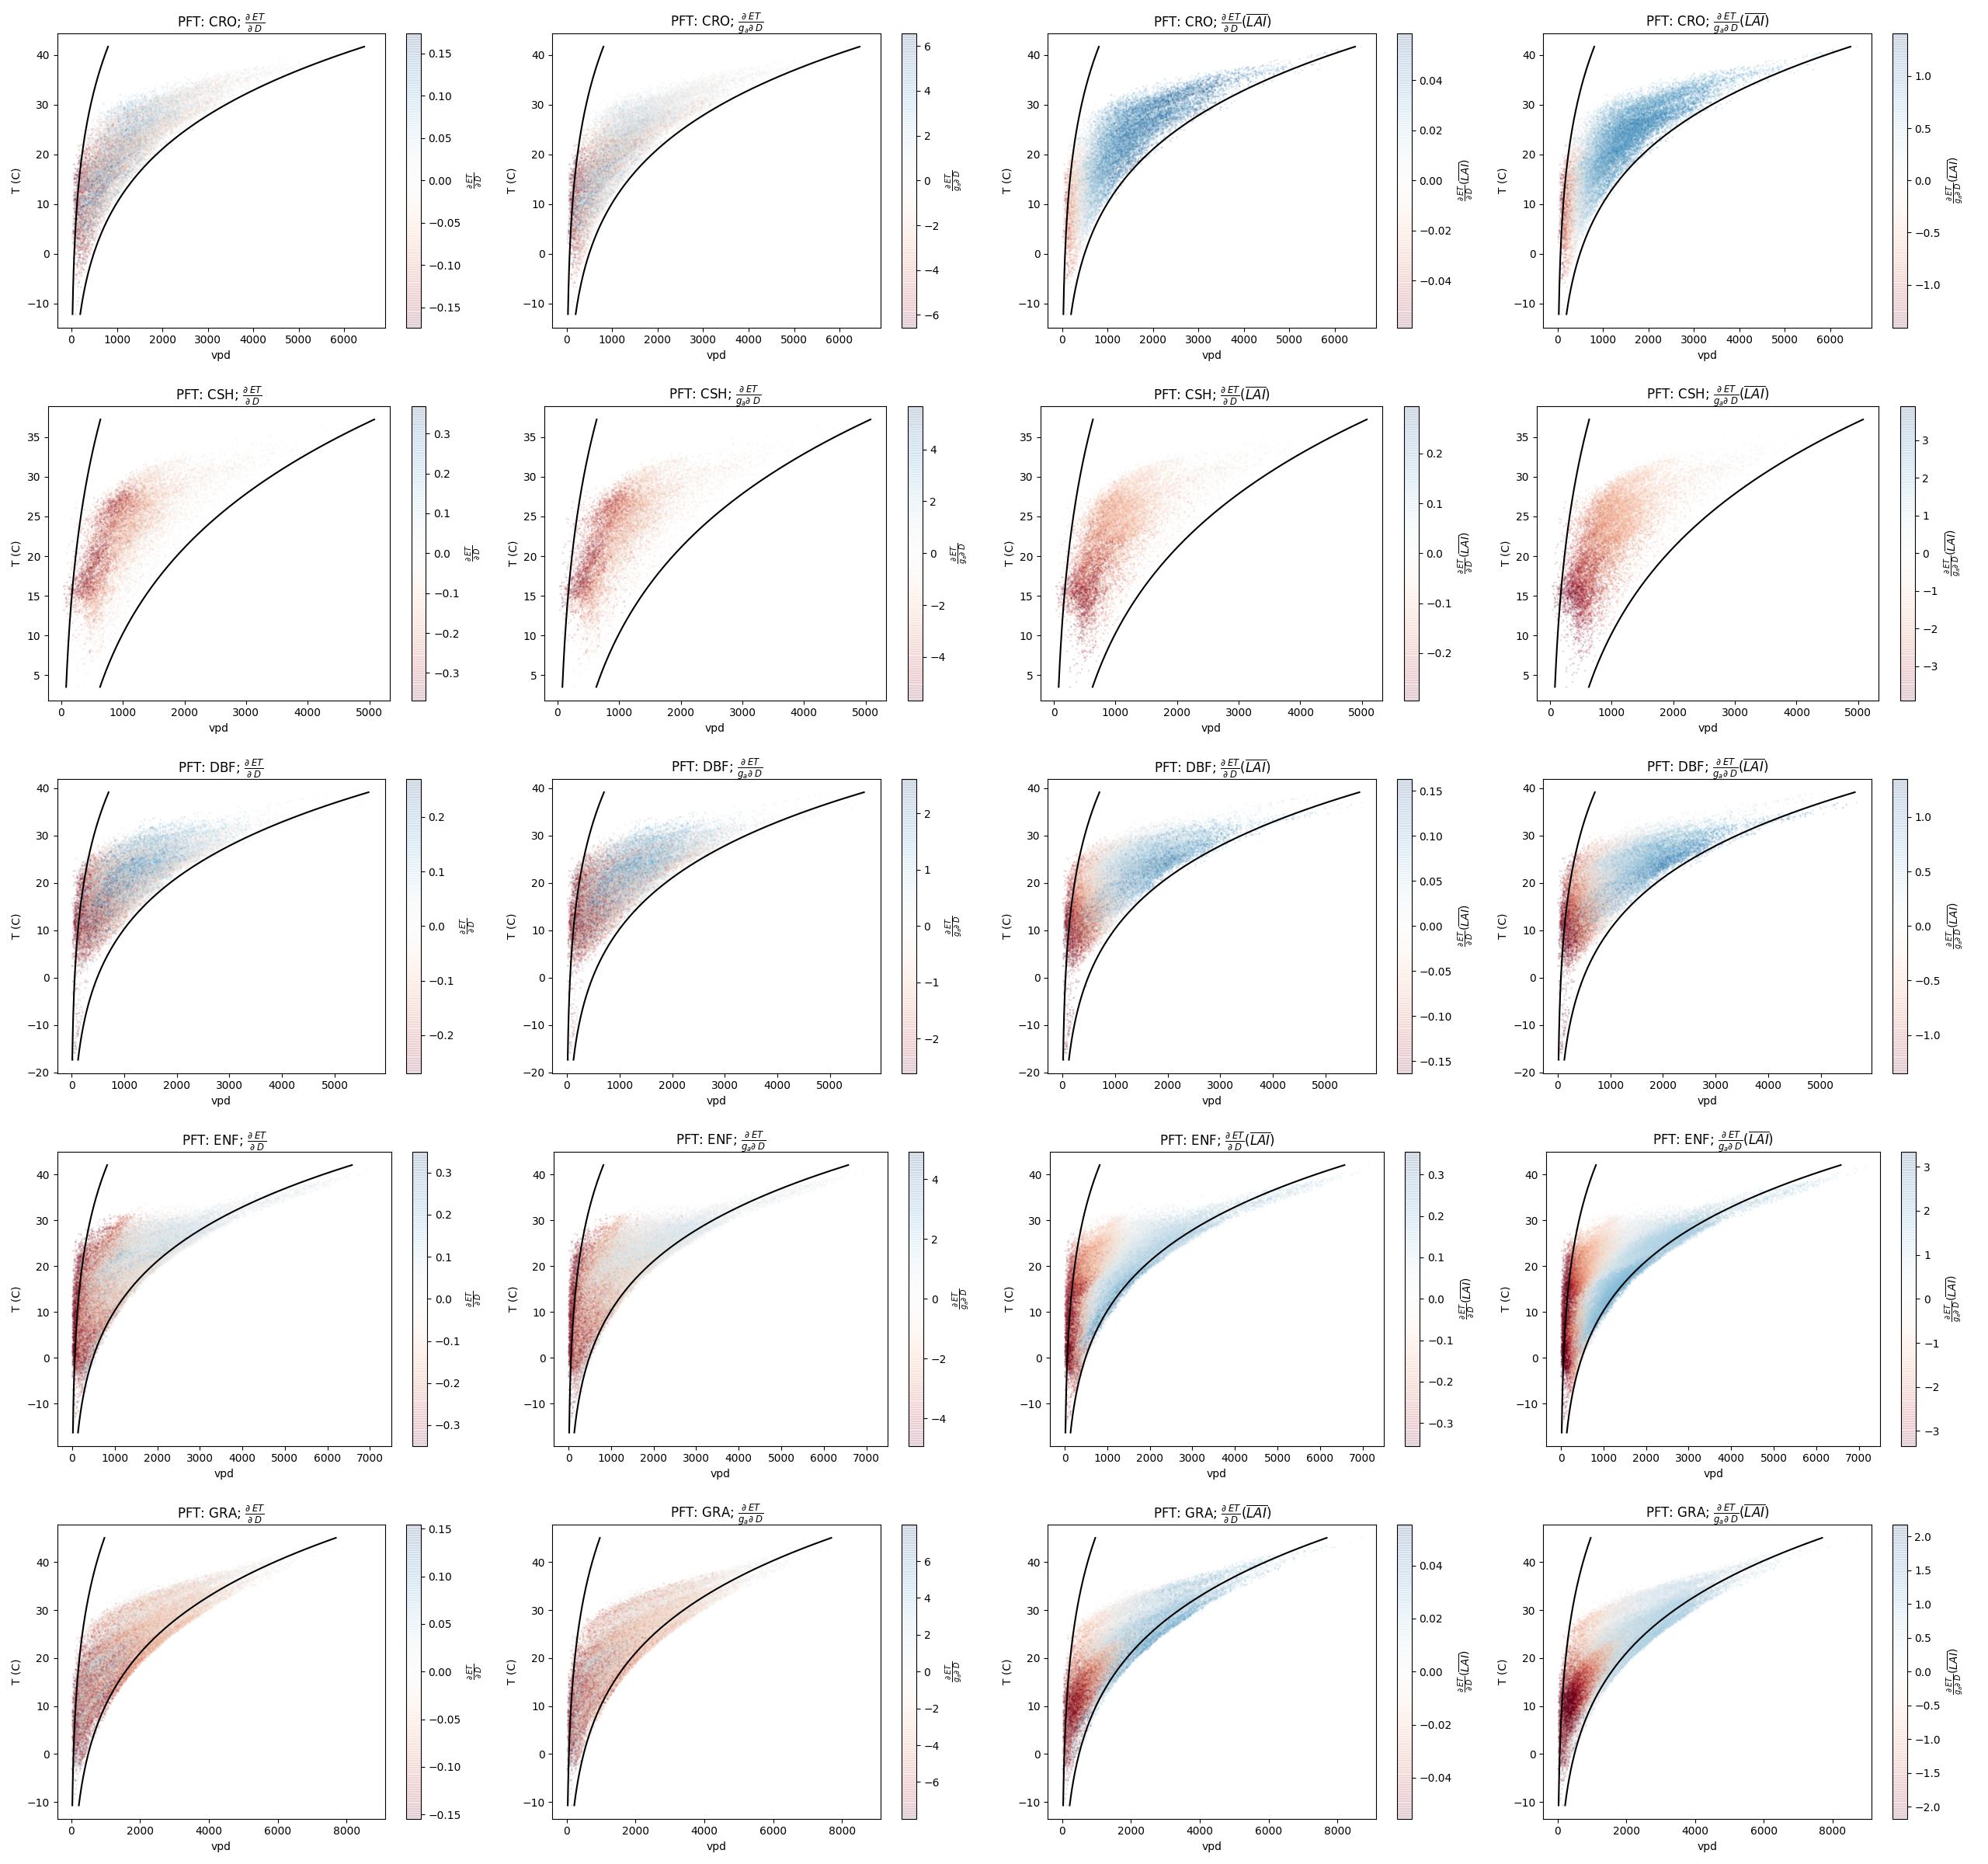
\includegraphics[width=1.4\textwidth]{./fig06.png}}
\caption{Scatter plots of $\frac{\partial \; ET}{\partial \; VPD}$. Each row is a different PFT, and each column is a different quantity related to $\frac{\partial \; ET}{\partial \; VPD}$, as labeled: Column 1: $\frac{\partial \; ET}{\partial \; VPD}$; Column 2: $\frac{\partial \; ET}{\partial \; VPD}$ normalized by $g_a$; Column 3: $\frac{\partial \; ET}{\partial \; VPD}$ with $\sigma$ held fixed at 1; and Column 4: $\frac{\partial \; ET}{\partial \; VPD}$ normalized by $g_a$ and with $\sigma$ held fixed. Please note differences in the colorbar scale.}
\label{real}
\end{figure}

% \begin{figure}[h]
% \centering
% 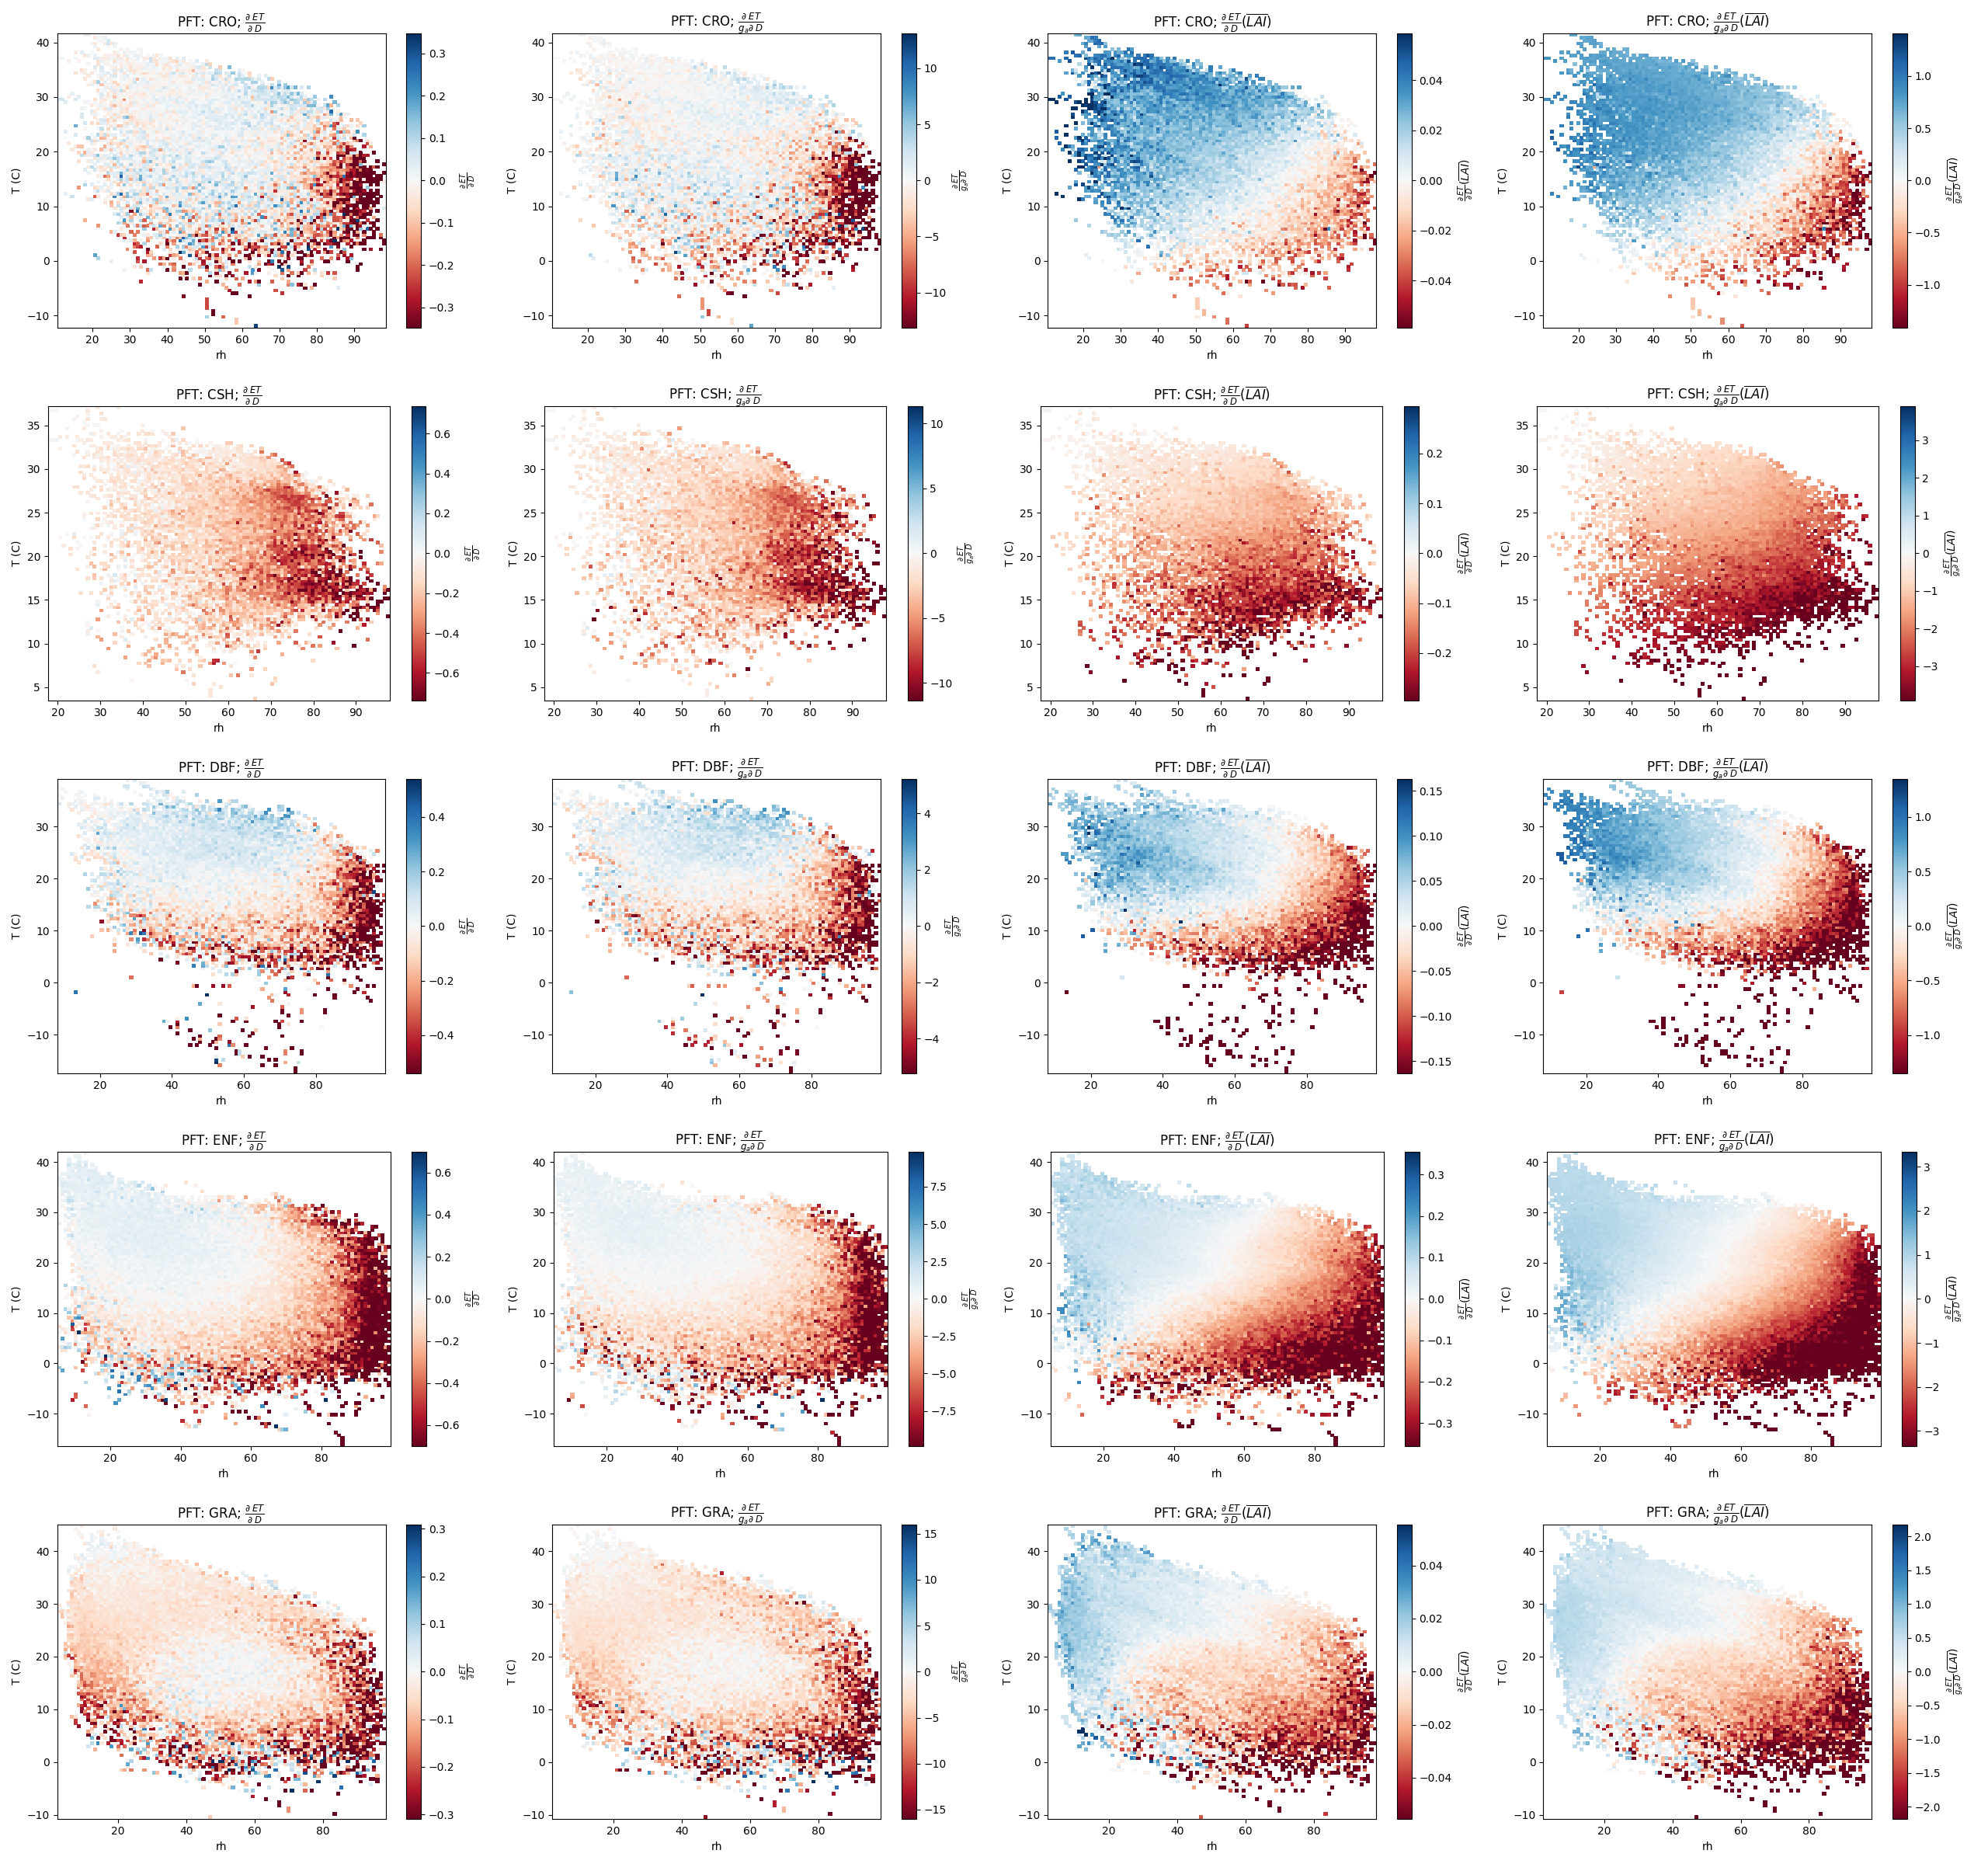
\includegraphics[width=\textwidth]{./fig06b.png}
% \caption{****alternate Fig 06****  Scatter plots of $\frac{\partial \; ET}{\partial \; VPD}$. Each row is a different PFT, and each column is a different quantity related to $\frac{\partial \; ET}{\partial \; VPD}$, as labeled. If I end up using this, I could also draw on the curve of $VPD_{crit}$ with $\overline{\frac{\text{LAI}}{\text{LAI$_{ref}$}}}$. }
% \label{real2}
% \end{figure}


\section{Limitations of theory}
\explain{HERE DISCUSS LIMITATION OF THE METHODS TO BVERY DRY CONDITIONS AND THE FEEDBCAK TO THE ATMOSPHERE OF VERY DRY SOIL CONDITIONS (BERG ET AL 2016, GENTINE ET AL> 2016)}

\section{Conclusions} 

We derived a new form of Penman Monteith using $uWUE$ (\cite{Zhou_2015}) to remove the stomatal conductance term's implicit dependence on ET. With our new form of Penman Monteith we developed a theory for when an ecosystem will tend to reduce or increase ET with increasing VPD. The goal was to capture the leading order behavior of the system to gain some intrinsic knowledge for its behavior. This intuition can be used to disentangle land atmosphere feedbacks in more complicated scenarios, and will aid interpretation of observations and sophisticated models.

Our theory states that each plant type has a critical VPD below which ET will decrease (plant response dominating) and above which ET will increase (atmospheric demand dominates). We tested our theory using data from FLUXNET 2015, and found that for DBF and CSH the theory succeeds in capturing the leading order behavior. For ENF, the theory succeeds in capturing the leading order behavior for the sign of $\frac{\partial \; ET}{\partial \; VPD}$, but not for magnitude. In contrast, the model does not capture the behavior for CRO and GRA. In some ways we should have expected this, as our theory does not account for large sources of variability we would expect for those plant types, including varying surface roughness, c3 vs c4 photosynthesis, and potential differences in irrigation across sites. Given these deficiencies for CRO and GRA, we will withhold conclusions on their response to increasing VPD.

For the forest sites (DBF, ENF) the observed environmental VPD approximately straddles the critical VPD, with about half the observations below the critical VPD and half above. However for CSH the environmental VPD never exceeds the critical VPD, and even when uncertainty is included the sign of the derivative is almost always negative (93\% of observations).

While our theory predicts common occurrence of positive $\frac{\partial \; ET}{\partial \; VPD}$ (atmospheric demand dominates), the plant response is still important even when $\frac{\partial \; ET}{\partial \; VPD} > 0$. The magnitude of the ``sign term'' of our theory is always far below what it would be if we only considered the atmospheric demand term (PET). This means that any drought indices or analysis using PET will not capture how the vegetated surface respond and react to increases in atmospheric demand. However, the new uWUE-version of Penman Monteith we derived (Equation \ref{et}) could be used as a complement to PET in drought indices. One could calculate and compare indices  when plant response is ignored (PET) or included (Equation \ref{et}). 

This paper provides initial intuition for how the land surface responds to atmospheric drying. This intuition for the one-way behavior of  land surface response to atmospheric drying is critical first step to disentangling land-atmosphere feedbacks at various scales, from diurnal to seasonal and beyond. 

%%
%% Enter Figures and Tables near as possible to where they are first mentioned:
%
% DO NOT USE \psfrag or \subfigure commands.
%
% Figure captions go below the figure.
% Table titles go above tables;  other caption information
%  should be placed in last line of the table, using
% \multicolumn2l{$^a$ This is a table note.}
%
%----------------
% EXAMPLE FIGURE
%
% \begin{figure}[h]
% \centering
% when using pdflatex, use pdf file:
% \includegraphics[width=20pc]{figsamp.pdf}
%
% when using dvips, use .eps file:
% \includegraphics[width=20pc]{figsamp.eps}
%
% \caption{Short caption}
% \label{figone}
%  \end{figure}
%
% ---------------
% EXAMPLE TABLE
%
% \begin{table}
% \caption{Time of the Transition Between Phase 1 and Phase 2$^{a}$}
% \centering
% \begin{tabular}{l c}
% \hline
%  Run  & Time (min)  \\
% \hline
%   $l1$  & 260   \\
%   $l2$  & 300   \\
%   $l3$  & 340   \\
%   $h1$  & 270   \\
%   $h2$  & 250   \\
%   $h3$  & 380   \\
%   $r1$  & 370   \\
%   $r2$  & 390   \\
% \hline
% \multicolumn{2}{l}{$^{a}$Footnote text here.}
% \end{tabular}
% \end{table}

%% SIDEWAYS FIGURE and TABLE 
% AGU prefers the use of {sidewaystable} over {landscapetable} as it causes fewer problems.
%
% \begin{sidewaysfigure}
% \includegraphics[width=20pc]{figsamp}
% \caption{caption here}
% \label{newfig}
% \end{sidewaysfigure}
% 
%  \begin{sidewaystable}
%  \caption{Caption here}
% \label{tab:signif_gap_clos}
%  \begin{tabular}{ccc}
% one&two&three\\
% four&five&six
%  \end{tabular}
%  \end{sidewaystable}

%% If using numbered lines, please surround equations with \begin{linenomath*}...\end{linenomath*}
%\begin{linenomath*}
%\begin{equation}
%y|{f} \sim g(m, \sigma),
%\end{equation}
%\end{linenomath*}

%%% End of body of article

%%%%%%%%%%%%%%%%%%%%%%%%%%%%%%%%
%% Optional Appendix goes here
%
% The \appendix command resets counters and redefines section heads
%
% After typing \appendix
%
%\section{Here Is Appendix Title}
% will show
% A: Here Is Appendix Title
%
%\appendix
%\section{Here is a sample appendix}

%%%%%%%%%%%%%%%%%%%%%%%%%%%%%%%%%%%%%%%%%%%%%%%%%%%%%%%%%%%%%%%%
%
% Optional Glossary, Notation or Acronym section goes here:
%
%%%%%%%%%%%%%%  
% Glossary is only allowed in Reviews of Geophysics
%  \begin{glossary}
%  \term{Term}
%   Term Definition here
%  \term{Term}
%   Term Definition here
%  \term{Term}
%   Term Definition here
%  \end{glossary}

%
%%%%%%%%%%%%%%
% Acronyms
%   \begin{acronyms}
%   \acro{Acronym}
%   Definition here
%   \acro{EMOS}
%   Ensemble model output statistics 
%   \acro{ECMWF}
%   Centre for Medium-Range Weather Forecasts
%   \end{acronyms}

%
%%%%%%%%%%%%%%
% Notation 
%   \begin{notation}
%   \notation{$a+b$} Notation Definition here
%   \notation{$e=mc^2$} 
%   Equation in German-born physicist Albert Einstein's theory of special
%  relativity that showed that the increased relativistic mass ($m$) of a
%  body comes from the energy of motion of the body—that is, its kinetic
%  energy ($E$)—divided by the speed of light squared ($c^2$).
%   \end{notation}




%%%%%%%%%%%%%%%%%%%%%%%%%%%%%%%%%%%%%%%%%%%%%%%%%%%%%%%%%%%%%%%%
%
%  ACKNOWLEDGMENTS
%
% The acknowledgments must list:
%
% •	All funding sources related to this work from all authors
%
% •	Any real or perceived financial conflicts of interests for any
%	author
%
% •	Other affiliations for any author that may be perceived as
% 	having a conflict of interest with respect to the results of this
% 	paper.
%
% •	A statement that indicates to the reader where the data
% 	supporting the conclusions can be obtained (for example, in the
% 	references, tables, supporting information, and other databases).
%
% It is also the appropriate place to thank colleagues and other contributors. 
% AGU does not normally allow dedications.


\acknowledgments
This work used eddy covariance data acquired and shared by the FLUXNET community, including these networks: AmeriFlux, AfriFlux, AsiaFlux, CarboAfrica, CarboEuropeIP, CarboItaly, CarboMont, ChinaFlux, Fluxnet-Canada, GreenGrass, ICOS, KoFlux, LBA, NECC, OzFlux-TERN, TCOS-Siberia, and USCCC. The ERA-Interim reanalysis data are provided by ECMWF and processed by LSCE. The FLUXNET eddy covariance data processing and harmonization was carried out by the European Fluxes Database Cluster, AmeriFlux Management Project, and Fluxdata project of FLUXNET, with the support of CDIAC and ICOS Ecosystem Thematic Center, and the OzFlux, ChinaFlux and AsiaFlux offices.


%% ------------------------------------------------------------------------ %%
%% Citations

% Please use ONLY \citet and \citep for reference citations.
% DO NOT use other cite commands (e.g., \cite, \citeyear, \nocite, \citealp, etc.).


%% Example \citet and \citep:
%  ...as shown by \citet{Boug10}, \citet{Buiz07}, \citet{Fra10},
%  \citet{Ghel00}, and \citet{Leit74}. 

%  ...as shown by \citep{Boug10}, \citep{Buiz07}, \citep{Fra10},
%  \citep{Ghel00, Leit74}. 

%  ...has been shown \citep [e.g.,][]{Boug10,Buiz07,Fra10}.



%%  REFERENCE LIST AND TEXT CITATIONS
%
% Either type in your references using
%
% \begin{thebibliography}{}
% \bibitem[{\textit{Kobayashi et~al.}}(2003)]{R2013} Kobayashi, T.,
% Tran, A.~H., Nishijo, H., Ono, T., and Matsumoto, G.  (2003).
% Contribution of hippocampal place cell activity to learning and
% formation of goal-directed navigation in rats. \textit{Neuroscience}
% 117, 1025--1035.
%
% \bibitem{}
% Text
% \end{thebibliography}
%
%%%%%%%%%%%%%%%%%%%%%%%%%%%%%%%%%%%%%%%%%%%%%%%
% Or, to use BibTeX:
%
% Follow these steps
%
% 1. Type in \bibliography{<name of your .bib file>} 
%    Run LaTeX on your LaTeX file.
%
% 2. Run BiBTeX on your LaTeX file.
%
% 3. Open the new .bbl file containing the reference list and
%   copy all the contents into your LaTeX file here.
%
% 4. Run LaTeX on your new file which will produce the citations.
%
% AGU does not want a .bib or a .bbl file. Please copy in the contents of your .bbl file here.
%\bibliography{references.bib}
\input{vpd_et_paper_PG_v1.bbl}


\listofchanges


\end{document}






\listofchanges


\end{document}






\listofchanges


\end{document}






\listofchanges


\end{document}



